\documentclass[twoside]{book}

% Packages required by doxygen
\usepackage{fixltx2e}
\usepackage{calc}
\usepackage{doxygen}
\usepackage[export]{adjustbox} % also loads graphicx
\usepackage{graphicx}
\usepackage[utf8]{inputenc}
\usepackage{makeidx}
\usepackage{multicol}
\usepackage{multirow}
\PassOptionsToPackage{warn}{textcomp}
\usepackage{textcomp}
\usepackage[nointegrals]{wasysym}
\usepackage[table]{xcolor}

% Font selection
\usepackage[T1]{fontenc}
\usepackage[scaled=.90]{helvet}
\usepackage{courier}
\usepackage{amssymb}
\usepackage{sectsty}
\renewcommand{\familydefault}{\sfdefault}
\allsectionsfont{%
  \fontseries{bc}\selectfont%
  \color{darkgray}%
}
\renewcommand{\DoxyLabelFont}{%
  \fontseries{bc}\selectfont%
  \color{darkgray}%
}
\newcommand{\+}{\discretionary{\mbox{\scriptsize$\hookleftarrow$}}{}{}}

% Page & text layout
\usepackage{geometry}
\geometry{%
  a4paper,%
  top=2.5cm,%
  bottom=2.5cm,%
  left=2.5cm,%
  right=2.5cm%
}
\tolerance=750
\hfuzz=15pt
\hbadness=750
\setlength{\emergencystretch}{15pt}
\setlength{\parindent}{0cm}
\setlength{\parskip}{3ex plus 2ex minus 2ex}
\makeatletter
\renewcommand{\paragraph}{%
  \@startsection{paragraph}{4}{0ex}{-1.0ex}{1.0ex}{%
    \normalfont\normalsize\bfseries\SS@parafont%
  }%
}
\renewcommand{\subparagraph}{%
  \@startsection{subparagraph}{5}{0ex}{-1.0ex}{1.0ex}{%
    \normalfont\normalsize\bfseries\SS@subparafont%
  }%
}
\makeatother

% Headers & footers
\usepackage{fancyhdr}
\pagestyle{fancyplain}
\fancyhead[LE]{\fancyplain{}{\bfseries\thepage}}
\fancyhead[CE]{\fancyplain{}{}}
\fancyhead[RE]{\fancyplain{}{\bfseries\leftmark}}
\fancyhead[LO]{\fancyplain{}{\bfseries\rightmark}}
\fancyhead[CO]{\fancyplain{}{}}
\fancyhead[RO]{\fancyplain{}{\bfseries\thepage}}
\fancyfoot[LE]{\fancyplain{}{}}
\fancyfoot[CE]{\fancyplain{}{}}
\fancyfoot[RE]{\fancyplain{}{\bfseries\scriptsize Generated by Doxygen }}
\fancyfoot[LO]{\fancyplain{}{\bfseries\scriptsize Generated by Doxygen }}
\fancyfoot[CO]{\fancyplain{}{}}
\fancyfoot[RO]{\fancyplain{}{}}
\renewcommand{\footrulewidth}{0.4pt}
\renewcommand{\chaptermark}[1]{%
  \markboth{#1}{}%
}
\renewcommand{\sectionmark}[1]{%
  \markright{\thesection\ #1}%
}

% Indices & bibliography
\usepackage{natbib}
\usepackage[titles]{tocloft}
\setcounter{tocdepth}{3}
\setcounter{secnumdepth}{5}
\makeindex

% Hyperlinks (required, but should be loaded last)
\usepackage{ifpdf}
\ifpdf
  \usepackage[pdftex,pagebackref=true]{hyperref}
\else
  \usepackage[ps2pdf,pagebackref=true]{hyperref}
\fi
\hypersetup{%
  colorlinks=true,%
  linkcolor=blue,%
  citecolor=blue,%
  unicode%
}

% Custom commands
\newcommand{\clearemptydoublepage}{%
  \newpage{\pagestyle{empty}\cleardoublepage}%
}

\usepackage{caption}
\captionsetup{labelsep=space,justification=centering,font={bf},singlelinecheck=off,skip=4pt,position=top}

%===== C O N T E N T S =====

\begin{document}

% Titlepage & ToC
\hypersetup{pageanchor=false,
             bookmarksnumbered=true,
             pdfencoding=unicode
            }
\pagenumbering{alph}
\begin{titlepage}
\vspace*{7cm}
\begin{center}%
{\Large My Project }\\
\vspace*{1cm}
{\large Generated by Doxygen 1.8.14}\\
\end{center}
\end{titlepage}
\clearemptydoublepage
\pagenumbering{roman}
\tableofcontents
\clearemptydoublepage
\pagenumbering{arabic}
\hypersetup{pageanchor=true}

%--- Begin generated contents ---
\chapter{Module Index}
\section{Modules}
Here is a list of all modules\+:\begin{DoxyCompactList}
\item \contentsline{section}{C\+M\+S\+IS}{\pageref{group___c_m_s_i_s}}{}
\begin{DoxyCompactList}
\item \contentsline{section}{Stm32f4xx\+\_\+system}{\pageref{group__stm32f4xx__system}}{}
\begin{DoxyCompactList}
\item \contentsline{section}{S\+T\+M32\+F4xx\+\_\+\+System\+\_\+\+Private\+\_\+\+Includes}{\pageref{group___s_t_m32_f4xx___system___private___includes}}{}
\item \contentsline{section}{S\+T\+M32\+F4xx\+\_\+\+System\+\_\+\+Private\+\_\+\+Types\+Definitions}{\pageref{group___s_t_m32_f4xx___system___private___types_definitions}}{}
\item \contentsline{section}{S\+T\+M32\+F4xx\+\_\+\+System\+\_\+\+Private\+\_\+\+Defines}{\pageref{group___s_t_m32_f4xx___system___private___defines}}{}
\item \contentsline{section}{S\+T\+M32\+F4xx\+\_\+\+System\+\_\+\+Private\+\_\+\+Macros}{\pageref{group___s_t_m32_f4xx___system___private___macros}}{}
\item \contentsline{section}{S\+T\+M32\+F4xx\+\_\+\+System\+\_\+\+Private\+\_\+\+Variables}{\pageref{group___s_t_m32_f4xx___system___private___variables}}{}
\item \contentsline{section}{S\+T\+M32\+F4xx\+\_\+\+System\+\_\+\+Private\+\_\+\+Function\+Prototypes}{\pageref{group___s_t_m32_f4xx___system___private___function_prototypes}}{}
\item \contentsline{section}{S\+T\+M32\+F4xx\+\_\+\+System\+\_\+\+Private\+\_\+\+Functions}{\pageref{group___s_t_m32_f4xx___system___private___functions}}{}
\end{DoxyCompactList}
\end{DoxyCompactList}
\end{DoxyCompactList}

\chapter{Data Structure Index}
\section{Data Structures}
Here are the data structures with brief descriptions\+:\begin{DoxyCompactList}
\item\contentsline{section}{\mbox{\hyperlink{struct_app_data__}{App\+Data\+\_\+}} }{\pageref{struct_app_data__}}{}
\item\contentsline{section}{\mbox{\hyperlink{struct_main_process_data__}{Main\+Process\+Data\+\_\+}} }{\pageref{struct_main_process_data__}}{}
\end{DoxyCompactList}

\chapter{File Index}
\section{File List}
Here is a list of all files with brief descriptions\+:\begin{DoxyCompactList}
\item\contentsline{section}{Src/\mbox{\hyperlink{button_8c}{button.\+c}} }{\pageref{button_8c}}{}
\item\contentsline{section}{Src/\mbox{\hyperlink{button__driver_8c}{button\+\_\+driver.\+c}} }{\pageref{button__driver_8c}}{}
\item\contentsline{section}{Src/\mbox{\hyperlink{gpio_8c}{gpio.\+c}} }{\pageref{gpio_8c}}{}
\item\contentsline{section}{Src/\mbox{\hyperlink{joystick_8c}{joystick.\+c}} }{\pageref{joystick_8c}}{}
\item\contentsline{section}{Src/\mbox{\hyperlink{lcd__driver_8c}{lcd\+\_\+driver.\+c}} }{\pageref{lcd__driver_8c}}{}
\item\contentsline{section}{Src/\mbox{\hyperlink{lcd__menu_8c}{lcd\+\_\+menu.\+c}} }{\pageref{lcd__menu_8c}}{}
\item\contentsline{section}{Src/\mbox{\hyperlink{main_8c}{main.\+c}} \\*\+: Main program body }{\pageref{main_8c}}{}
\item\contentsline{section}{Src/\mbox{\hyperlink{spi_8c}{spi.\+c}} }{\pageref{spi_8c}}{}
\item\contentsline{section}{Src/\mbox{\hyperlink{stm32f4xx__hal__msp_8c}{stm32f4xx\+\_\+hal\+\_\+msp.\+c}} }{\pageref{stm32f4xx__hal__msp_8c}}{}
\item\contentsline{section}{Src/\mbox{\hyperlink{stm32f4xx__it_8c}{stm32f4xx\+\_\+it.\+c}} \\*Interrupt Service Routines }{\pageref{stm32f4xx__it_8c}}{}
\item\contentsline{section}{Src/\mbox{\hyperlink{system__stm32f4xx_8c}{system\+\_\+stm32f4xx.\+c}} \\*C\+M\+S\+IS Cortex-\/\+M4 Device Peripheral Access Layer System Source File }{\pageref{system__stm32f4xx_8c}}{}
\item\contentsline{section}{Src/\mbox{\hyperlink{tmc260_8c}{tmc260.\+c}} }{\pageref{tmc260_8c}}{}
\item\contentsline{section}{Src/\mbox{\hyperlink{tmc260__driver_8c}{tmc260\+\_\+driver.\+c}} }{\pageref{tmc260__driver_8c}}{}
\end{DoxyCompactList}

\chapter{Module Documentation}
\hypertarget{group___c_m_s_i_s}{}\section{C\+M\+S\+IS}
\label{group___c_m_s_i_s}\index{C\+M\+S\+IS@{C\+M\+S\+IS}}
Collaboration diagram for C\+M\+S\+IS\+:
\nopagebreak
\begin{figure}[H]
\begin{center}
\leavevmode
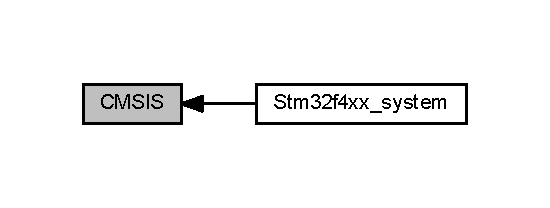
\includegraphics[width=264pt]{group___c_m_s_i_s}
\end{center}
\end{figure}
\subsection*{Modules}
\begin{DoxyCompactItemize}
\item 
\mbox{\hyperlink{group__stm32f4xx__system}{Stm32f4xx\+\_\+system}}
\end{DoxyCompactItemize}


\subsection{Detailed Description}

\hypertarget{group__stm32f4xx__system}{}\section{Stm32f4xx\+\_\+system}
\label{group__stm32f4xx__system}\index{Stm32f4xx\+\_\+system@{Stm32f4xx\+\_\+system}}
Collaboration diagram for Stm32f4xx\+\_\+system\+:
\nopagebreak
\begin{figure}[H]
\begin{center}
\leavevmode
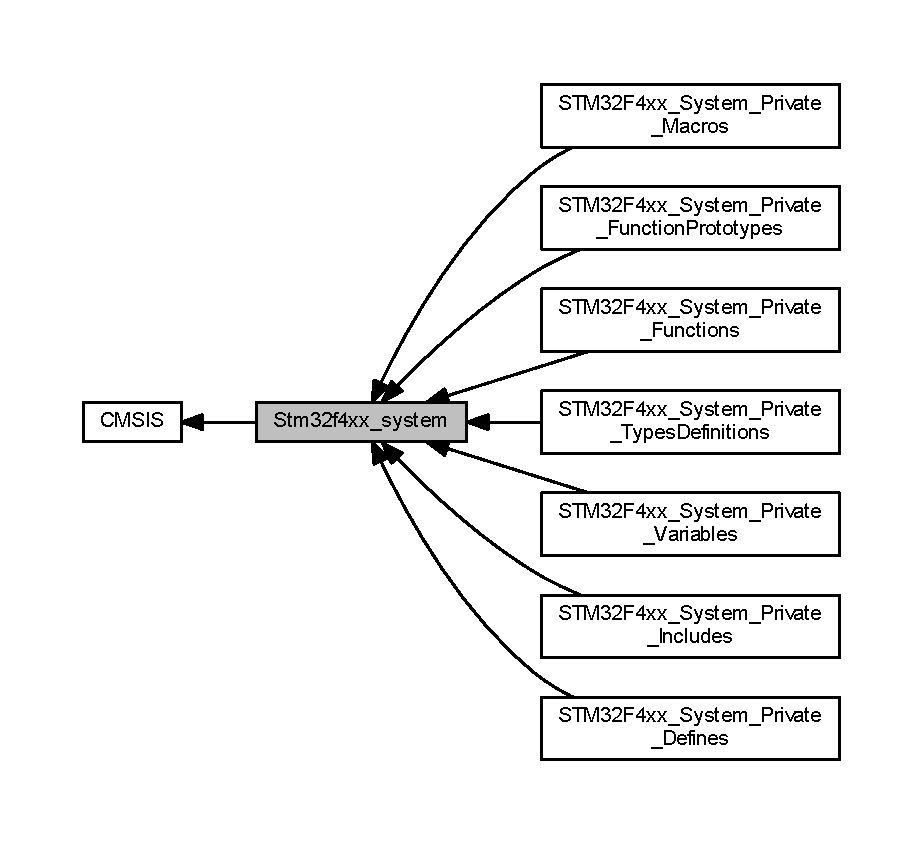
\includegraphics[width=350pt]{group__stm32f4xx__system}
\end{center}
\end{figure}
\subsection*{Modules}
\begin{DoxyCompactItemize}
\item 
\mbox{\hyperlink{group___s_t_m32_f4xx___system___private___includes}{S\+T\+M32\+F4xx\+\_\+\+System\+\_\+\+Private\+\_\+\+Includes}}
\item 
\mbox{\hyperlink{group___s_t_m32_f4xx___system___private___types_definitions}{S\+T\+M32\+F4xx\+\_\+\+System\+\_\+\+Private\+\_\+\+Types\+Definitions}}
\item 
\mbox{\hyperlink{group___s_t_m32_f4xx___system___private___defines}{S\+T\+M32\+F4xx\+\_\+\+System\+\_\+\+Private\+\_\+\+Defines}}
\item 
\mbox{\hyperlink{group___s_t_m32_f4xx___system___private___macros}{S\+T\+M32\+F4xx\+\_\+\+System\+\_\+\+Private\+\_\+\+Macros}}
\item 
\mbox{\hyperlink{group___s_t_m32_f4xx___system___private___variables}{S\+T\+M32\+F4xx\+\_\+\+System\+\_\+\+Private\+\_\+\+Variables}}
\item 
\mbox{\hyperlink{group___s_t_m32_f4xx___system___private___function_prototypes}{S\+T\+M32\+F4xx\+\_\+\+System\+\_\+\+Private\+\_\+\+Function\+Prototypes}}
\item 
\mbox{\hyperlink{group___s_t_m32_f4xx___system___private___functions}{S\+T\+M32\+F4xx\+\_\+\+System\+\_\+\+Private\+\_\+\+Functions}}
\end{DoxyCompactItemize}


\subsection{Detailed Description}

\hypertarget{group___s_t_m32_f4xx___system___private___includes}{}\section{S\+T\+M32\+F4xx\+\_\+\+System\+\_\+\+Private\+\_\+\+Includes}
\label{group___s_t_m32_f4xx___system___private___includes}\index{S\+T\+M32\+F4xx\+\_\+\+System\+\_\+\+Private\+\_\+\+Includes@{S\+T\+M32\+F4xx\+\_\+\+System\+\_\+\+Private\+\_\+\+Includes}}
Collaboration diagram for S\+T\+M32\+F4xx\+\_\+\+System\+\_\+\+Private\+\_\+\+Includes\+:\nopagebreak
\begin{figure}[H]
\begin{center}
\leavevmode
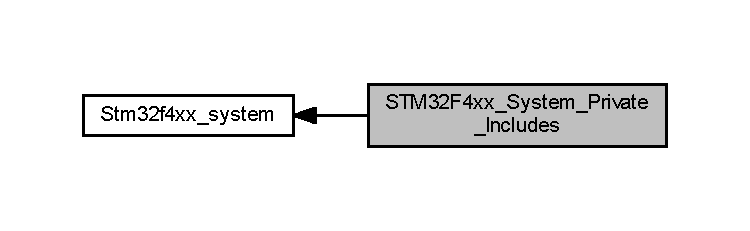
\includegraphics[width=350pt]{group___s_t_m32_f4xx___system___private___includes}
\end{center}
\end{figure}
\subsection*{Macros}
\begin{DoxyCompactItemize}
\item 
\#define \mbox{\hyperlink{group___s_t_m32_f4xx___system___private___includes_gaeafcff4f57440c60e64812dddd13e7cb}{H\+S\+E\+\_\+\+V\+A\+L\+UE}}~((uint32\+\_\+t)25000000)
\item 
\#define \mbox{\hyperlink{group___s_t_m32_f4xx___system___private___includes_gaaa8c76e274d0f6dd2cefb5d0b17fbc37}{H\+S\+I\+\_\+\+V\+A\+L\+UE}}~((uint32\+\_\+t)16000000)
\end{DoxyCompactItemize}


\subsection{Detailed Description}


\subsection{Macro Definition Documentation}
\mbox{\Hypertarget{group___s_t_m32_f4xx___system___private___includes_gaeafcff4f57440c60e64812dddd13e7cb}\label{group___s_t_m32_f4xx___system___private___includes_gaeafcff4f57440c60e64812dddd13e7cb}} 
\index{S\+T\+M32\+F4xx\+\_\+\+System\+\_\+\+Private\+\_\+\+Includes@{S\+T\+M32\+F4xx\+\_\+\+System\+\_\+\+Private\+\_\+\+Includes}!H\+S\+E\+\_\+\+V\+A\+L\+UE@{H\+S\+E\+\_\+\+V\+A\+L\+UE}}
\index{H\+S\+E\+\_\+\+V\+A\+L\+UE@{H\+S\+E\+\_\+\+V\+A\+L\+UE}!S\+T\+M32\+F4xx\+\_\+\+System\+\_\+\+Private\+\_\+\+Includes@{S\+T\+M32\+F4xx\+\_\+\+System\+\_\+\+Private\+\_\+\+Includes}}
\subsubsection{\texorpdfstring{H\+S\+E\+\_\+\+V\+A\+L\+UE}{HSE\_VALUE}}
{\footnotesize\ttfamily \#define H\+S\+E\+\_\+\+V\+A\+L\+UE~((uint32\+\_\+t)25000000)}

Default value of the External oscillator in Hz 

Definition at line 68 of file system\+\_\+stm32f4xx.\+c.

\mbox{\Hypertarget{group___s_t_m32_f4xx___system___private___includes_gaaa8c76e274d0f6dd2cefb5d0b17fbc37}\label{group___s_t_m32_f4xx___system___private___includes_gaaa8c76e274d0f6dd2cefb5d0b17fbc37}} 
\index{S\+T\+M32\+F4xx\+\_\+\+System\+\_\+\+Private\+\_\+\+Includes@{S\+T\+M32\+F4xx\+\_\+\+System\+\_\+\+Private\+\_\+\+Includes}!H\+S\+I\+\_\+\+V\+A\+L\+UE@{H\+S\+I\+\_\+\+V\+A\+L\+UE}}
\index{H\+S\+I\+\_\+\+V\+A\+L\+UE@{H\+S\+I\+\_\+\+V\+A\+L\+UE}!S\+T\+M32\+F4xx\+\_\+\+System\+\_\+\+Private\+\_\+\+Includes@{S\+T\+M32\+F4xx\+\_\+\+System\+\_\+\+Private\+\_\+\+Includes}}
\subsubsection{\texorpdfstring{H\+S\+I\+\_\+\+V\+A\+L\+UE}{HSI\_VALUE}}
{\footnotesize\ttfamily \#define H\+S\+I\+\_\+\+V\+A\+L\+UE~((uint32\+\_\+t)16000000)}

Value of the Internal oscillator in Hz 

Definition at line 72 of file system\+\_\+stm32f4xx.\+c.


\hypertarget{group___s_t_m32_f4xx___system___private___types_definitions}{}\section{S\+T\+M32\+F4xx\+\_\+\+System\+\_\+\+Private\+\_\+\+Types\+Definitions}
\label{group___s_t_m32_f4xx___system___private___types_definitions}\index{S\+T\+M32\+F4xx\+\_\+\+System\+\_\+\+Private\+\_\+\+Types\+Definitions@{S\+T\+M32\+F4xx\+\_\+\+System\+\_\+\+Private\+\_\+\+Types\+Definitions}}
Collaboration diagram for S\+T\+M32\+F4xx\+\_\+\+System\+\_\+\+Private\+\_\+\+Types\+Definitions\+:
\nopagebreak
\begin{figure}[H]
\begin{center}
\leavevmode
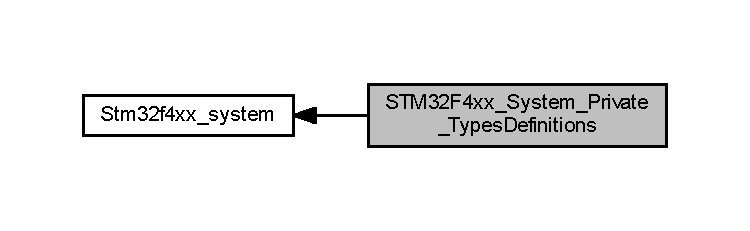
\includegraphics[width=350pt]{group___s_t_m32_f4xx___system___private___types_definitions}
\end{center}
\end{figure}

\hypertarget{group___s_t_m32_f4xx___system___private___defines}{}\section{S\+T\+M32\+F4xx\+\_\+\+System\+\_\+\+Private\+\_\+\+Defines}
\label{group___s_t_m32_f4xx___system___private___defines}\index{S\+T\+M32\+F4xx\+\_\+\+System\+\_\+\+Private\+\_\+\+Defines@{S\+T\+M32\+F4xx\+\_\+\+System\+\_\+\+Private\+\_\+\+Defines}}
Collaboration diagram for S\+T\+M32\+F4xx\+\_\+\+System\+\_\+\+Private\+\_\+\+Defines\+:\nopagebreak
\begin{figure}[H]
\begin{center}
\leavevmode
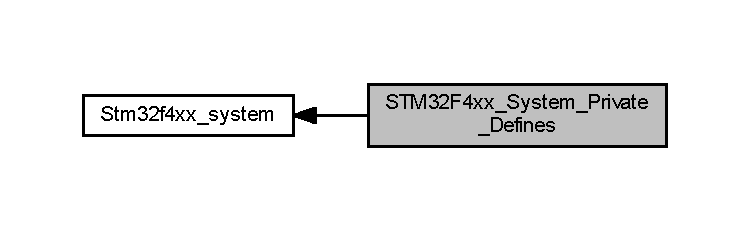
\includegraphics[width=350pt]{group___s_t_m32_f4xx___system___private___defines}
\end{center}
\end{figure}
\subsection*{Macros}
\begin{DoxyCompactItemize}
\item 
\#define \mbox{\hyperlink{group___s_t_m32_f4xx___system___private___defines_ga40e1495541cbb4acbe3f1819bd87a9fe}{V\+E\+C\+T\+\_\+\+T\+A\+B\+\_\+\+O\+F\+F\+S\+ET}}~0x00
\end{DoxyCompactItemize}


\subsection{Detailed Description}


\subsection{Macro Definition Documentation}
\mbox{\Hypertarget{group___s_t_m32_f4xx___system___private___defines_ga40e1495541cbb4acbe3f1819bd87a9fe}\label{group___s_t_m32_f4xx___system___private___defines_ga40e1495541cbb4acbe3f1819bd87a9fe}} 
\index{S\+T\+M32\+F4xx\+\_\+\+System\+\_\+\+Private\+\_\+\+Defines@{S\+T\+M32\+F4xx\+\_\+\+System\+\_\+\+Private\+\_\+\+Defines}!V\+E\+C\+T\+\_\+\+T\+A\+B\+\_\+\+O\+F\+F\+S\+ET@{V\+E\+C\+T\+\_\+\+T\+A\+B\+\_\+\+O\+F\+F\+S\+ET}}
\index{V\+E\+C\+T\+\_\+\+T\+A\+B\+\_\+\+O\+F\+F\+S\+ET@{V\+E\+C\+T\+\_\+\+T\+A\+B\+\_\+\+O\+F\+F\+S\+ET}!S\+T\+M32\+F4xx\+\_\+\+System\+\_\+\+Private\+\_\+\+Defines@{S\+T\+M32\+F4xx\+\_\+\+System\+\_\+\+Private\+\_\+\+Defines}}
\subsubsection{\texorpdfstring{V\+E\+C\+T\+\_\+\+T\+A\+B\+\_\+\+O\+F\+F\+S\+ET}{VECT\_TAB\_OFFSET}}
{\footnotesize\ttfamily \#define V\+E\+C\+T\+\_\+\+T\+A\+B\+\_\+\+O\+F\+F\+S\+ET~0x00}

$<$ Uncomment the following line if you need to use external S\+R\+AM or S\+D\+R\+AM as data memory ~\newline
~\newline
 $<$ Uncomment the following line if you need to relocate your vector \mbox{\hyperlink{struct_table}{Table}} in Internal S\+R\+AM. Vector \mbox{\hyperlink{struct_table}{Table}} base offset field. This value must be a multiple of 0x200. 

Definition at line 109 of file system\+\_\+stm32f4xx.\+c.


\hypertarget{group___s_t_m32_f4xx___system___private___macros}{}\section{S\+T\+M32\+F4xx\+\_\+\+System\+\_\+\+Private\+\_\+\+Macros}
\label{group___s_t_m32_f4xx___system___private___macros}\index{S\+T\+M32\+F4xx\+\_\+\+System\+\_\+\+Private\+\_\+\+Macros@{S\+T\+M32\+F4xx\+\_\+\+System\+\_\+\+Private\+\_\+\+Macros}}
Collaboration diagram for S\+T\+M32\+F4xx\+\_\+\+System\+\_\+\+Private\+\_\+\+Macros\+:\nopagebreak
\begin{figure}[H]
\begin{center}
\leavevmode
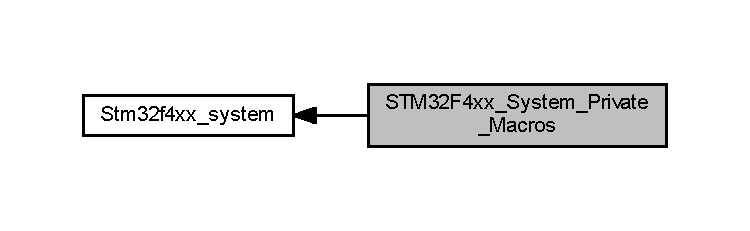
\includegraphics[width=350pt]{group___s_t_m32_f4xx___system___private___macros}
\end{center}
\end{figure}

\hypertarget{group___s_t_m32_f4xx___system___private___variables}{}\section{S\+T\+M32\+F4xx\+\_\+\+System\+\_\+\+Private\+\_\+\+Variables}
\label{group___s_t_m32_f4xx___system___private___variables}\index{S\+T\+M32\+F4xx\+\_\+\+System\+\_\+\+Private\+\_\+\+Variables@{S\+T\+M32\+F4xx\+\_\+\+System\+\_\+\+Private\+\_\+\+Variables}}
Collaboration diagram for S\+T\+M32\+F4xx\+\_\+\+System\+\_\+\+Private\+\_\+\+Variables\+:
\nopagebreak
\begin{figure}[H]
\begin{center}
\leavevmode
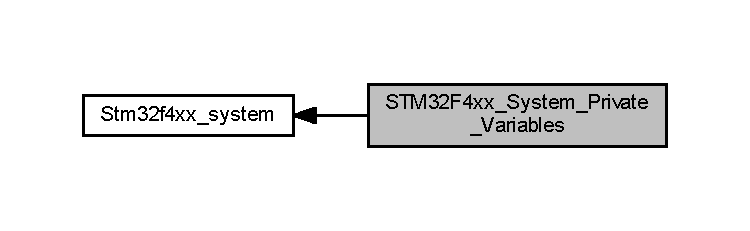
\includegraphics[width=350pt]{group___s_t_m32_f4xx___system___private___variables}
\end{center}
\end{figure}
\subsection*{Variables}
\begin{DoxyCompactItemize}
\item 
uint32\+\_\+t \mbox{\hyperlink{group___s_t_m32_f4xx___system___private___variables_gaa3cd3e43291e81e795d642b79b6088e6}{System\+Core\+Clock}} = 16000000
\item 
const uint8\+\_\+t \mbox{\hyperlink{group___s_t_m32_f4xx___system___private___variables_ga6e1d9cd666f0eacbfde31e9932a93466}{A\+H\+B\+Presc\+Table}} \mbox{[}16\mbox{]} = \{0, 0, 0, 0, 0, 0, 0, 0, 1, 2, 3, 4, 6, 7, 8, 9\}
\item 
const uint8\+\_\+t \mbox{\hyperlink{group___s_t_m32_f4xx___system___private___variables_ga5b4f8b768465842cf854a8f993b375e9}{A\+P\+B\+Presc\+Table}} \mbox{[}8\mbox{]} = \{0, 0, 0, 0, 1, 2, 3, 4\}
\end{DoxyCompactItemize}


\subsection{Detailed Description}


\subsection{Variable Documentation}
\mbox{\Hypertarget{group___s_t_m32_f4xx___system___private___variables_ga6e1d9cd666f0eacbfde31e9932a93466}\label{group___s_t_m32_f4xx___system___private___variables_ga6e1d9cd666f0eacbfde31e9932a93466}} 
\index{S\+T\+M32\+F4xx\+\_\+\+System\+\_\+\+Private\+\_\+\+Variables@{S\+T\+M32\+F4xx\+\_\+\+System\+\_\+\+Private\+\_\+\+Variables}!A\+H\+B\+Presc\+Table@{A\+H\+B\+Presc\+Table}}
\index{A\+H\+B\+Presc\+Table@{A\+H\+B\+Presc\+Table}!S\+T\+M32\+F4xx\+\_\+\+System\+\_\+\+Private\+\_\+\+Variables@{S\+T\+M32\+F4xx\+\_\+\+System\+\_\+\+Private\+\_\+\+Variables}}
\subsubsection{\texorpdfstring{A\+H\+B\+Presc\+Table}{AHBPrescTable}}
{\footnotesize\ttfamily const uint8\+\_\+t A\+H\+B\+Presc\+Table\mbox{[}16\mbox{]} = \{0, 0, 0, 0, 0, 0, 0, 0, 1, 2, 3, 4, 6, 7, 8, 9\}}



Definition at line 138 of file system\+\_\+stm32f4xx.\+c.

\mbox{\Hypertarget{group___s_t_m32_f4xx___system___private___variables_ga5b4f8b768465842cf854a8f993b375e9}\label{group___s_t_m32_f4xx___system___private___variables_ga5b4f8b768465842cf854a8f993b375e9}} 
\index{S\+T\+M32\+F4xx\+\_\+\+System\+\_\+\+Private\+\_\+\+Variables@{S\+T\+M32\+F4xx\+\_\+\+System\+\_\+\+Private\+\_\+\+Variables}!A\+P\+B\+Presc\+Table@{A\+P\+B\+Presc\+Table}}
\index{A\+P\+B\+Presc\+Table@{A\+P\+B\+Presc\+Table}!S\+T\+M32\+F4xx\+\_\+\+System\+\_\+\+Private\+\_\+\+Variables@{S\+T\+M32\+F4xx\+\_\+\+System\+\_\+\+Private\+\_\+\+Variables}}
\subsubsection{\texorpdfstring{A\+P\+B\+Presc\+Table}{APBPrescTable}}
{\footnotesize\ttfamily const uint8\+\_\+t A\+P\+B\+Presc\+Table\mbox{[}8\mbox{]} = \{0, 0, 0, 0, 1, 2, 3, 4\}}



Definition at line 139 of file system\+\_\+stm32f4xx.\+c.

\mbox{\Hypertarget{group___s_t_m32_f4xx___system___private___variables_gaa3cd3e43291e81e795d642b79b6088e6}\label{group___s_t_m32_f4xx___system___private___variables_gaa3cd3e43291e81e795d642b79b6088e6}} 
\index{S\+T\+M32\+F4xx\+\_\+\+System\+\_\+\+Private\+\_\+\+Variables@{S\+T\+M32\+F4xx\+\_\+\+System\+\_\+\+Private\+\_\+\+Variables}!System\+Core\+Clock@{System\+Core\+Clock}}
\index{System\+Core\+Clock@{System\+Core\+Clock}!S\+T\+M32\+F4xx\+\_\+\+System\+\_\+\+Private\+\_\+\+Variables@{S\+T\+M32\+F4xx\+\_\+\+System\+\_\+\+Private\+\_\+\+Variables}}
\subsubsection{\texorpdfstring{System\+Core\+Clock}{SystemCoreClock}}
{\footnotesize\ttfamily uint32\+\_\+t System\+Core\+Clock = 16000000}



Definition at line 137 of file system\+\_\+stm32f4xx.\+c.


\hypertarget{group___s_t_m32_f4xx___system___private___function_prototypes}{}\section{S\+T\+M32\+F4xx\+\_\+\+System\+\_\+\+Private\+\_\+\+Function\+Prototypes}
\label{group___s_t_m32_f4xx___system___private___function_prototypes}\index{S\+T\+M32\+F4xx\+\_\+\+System\+\_\+\+Private\+\_\+\+Function\+Prototypes@{S\+T\+M32\+F4xx\+\_\+\+System\+\_\+\+Private\+\_\+\+Function\+Prototypes}}
Collaboration diagram for S\+T\+M32\+F4xx\+\_\+\+System\+\_\+\+Private\+\_\+\+Function\+Prototypes\+:
\nopagebreak
\begin{figure}[H]
\begin{center}
\leavevmode
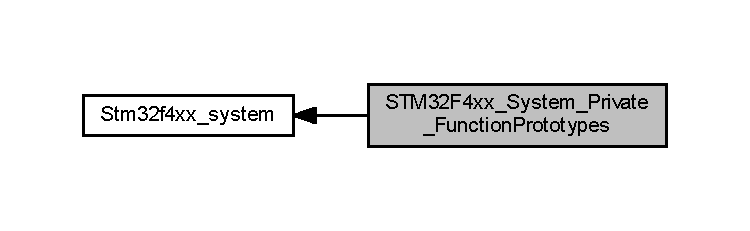
\includegraphics[width=350pt]{group___s_t_m32_f4xx___system___private___function_prototypes}
\end{center}
\end{figure}

\hypertarget{group___s_t_m32_f4xx___system___private___functions}{}\section{S\+T\+M32\+F4xx\+\_\+\+System\+\_\+\+Private\+\_\+\+Functions}
\label{group___s_t_m32_f4xx___system___private___functions}\index{S\+T\+M32\+F4xx\+\_\+\+System\+\_\+\+Private\+\_\+\+Functions@{S\+T\+M32\+F4xx\+\_\+\+System\+\_\+\+Private\+\_\+\+Functions}}
Collaboration diagram for S\+T\+M32\+F4xx\+\_\+\+System\+\_\+\+Private\+\_\+\+Functions\+:\nopagebreak
\begin{figure}[H]
\begin{center}
\leavevmode
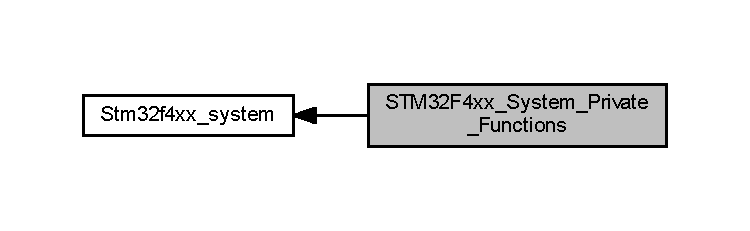
\includegraphics[width=350pt]{group___s_t_m32_f4xx___system___private___functions}
\end{center}
\end{figure}
\subsection*{Functions}
\begin{DoxyCompactItemize}
\item 
void \mbox{\hyperlink{group___s_t_m32_f4xx___system___private___functions_ga93f514700ccf00d08dbdcff7f1224eb2}{System\+Init}} (void)
\begin{DoxyCompactList}\small\item\em Setup the microcontroller system Initialize the F\+PU setting, vector table location and External memory configuration. \end{DoxyCompactList}\item 
void \mbox{\hyperlink{group___s_t_m32_f4xx___system___private___functions_gae0c36a9591fe6e9c45ecb21a794f0f0f}{System\+Core\+Clock\+Update}} (void)
\begin{DoxyCompactList}\small\item\em Update System\+Core\+Clock variable according to Clock Register Values. The System\+Core\+Clock variable contains the core clock (H\+C\+LK), it can be used by the user application to setup the Sys\+Tick timer or configure other parameters. \end{DoxyCompactList}\end{DoxyCompactItemize}


\subsection{Detailed Description}


\subsection{Function Documentation}
\mbox{\Hypertarget{group___s_t_m32_f4xx___system___private___functions_gae0c36a9591fe6e9c45ecb21a794f0f0f}\label{group___s_t_m32_f4xx___system___private___functions_gae0c36a9591fe6e9c45ecb21a794f0f0f}} 
\index{S\+T\+M32\+F4xx\+\_\+\+System\+\_\+\+Private\+\_\+\+Functions@{S\+T\+M32\+F4xx\+\_\+\+System\+\_\+\+Private\+\_\+\+Functions}!System\+Core\+Clock\+Update@{System\+Core\+Clock\+Update}}
\index{System\+Core\+Clock\+Update@{System\+Core\+Clock\+Update}!S\+T\+M32\+F4xx\+\_\+\+System\+\_\+\+Private\+\_\+\+Functions@{S\+T\+M32\+F4xx\+\_\+\+System\+\_\+\+Private\+\_\+\+Functions}}
\subsubsection{\texorpdfstring{System\+Core\+Clock\+Update()}{SystemCoreClockUpdate()}}
{\footnotesize\ttfamily void System\+Core\+Clock\+Update (\begin{DoxyParamCaption}\item[{void}]{ }\end{DoxyParamCaption})}



Update System\+Core\+Clock variable according to Clock Register Values. The System\+Core\+Clock variable contains the core clock (H\+C\+LK), it can be used by the user application to setup the Sys\+Tick timer or configure other parameters. 

\begin{DoxyNote}{Note}
Each time the core clock (H\+C\+LK) changes, this function must be called to update System\+Core\+Clock variable value. Otherwise, any configuration based on this variable will be incorrect. ~\newline
 

-\/ The system frequency computed by this function is not the real frequency in the chip. It is calculated based on the predefined constant and the selected clock source\+:
\end{DoxyNote}

\begin{DoxyItemize}
\item If S\+Y\+S\+C\+LK source is H\+SI, System\+Core\+Clock will contain the \mbox{\hyperlink{group___s_t_m32_f4xx___system___private___includes_gaaa8c76e274d0f6dd2cefb5d0b17fbc37}{H\+S\+I\+\_\+\+V\+A\+L\+U\+E($\ast$)}}
\item If S\+Y\+S\+C\+LK source is H\+SE, System\+Core\+Clock will contain the \mbox{\hyperlink{group___s_t_m32_f4xx___system___private___includes_gaeafcff4f57440c60e64812dddd13e7cb}{H\+S\+E\+\_\+\+V\+A\+L\+U\+E($\ast$$\ast$)}}
\item If S\+Y\+S\+C\+LK source is P\+LL, System\+Core\+Clock will contain the \mbox{\hyperlink{group___s_t_m32_f4xx___system___private___includes_gaeafcff4f57440c60e64812dddd13e7cb}{H\+S\+E\+\_\+\+V\+A\+L\+U\+E($\ast$$\ast$)}} or \mbox{\hyperlink{group___s_t_m32_f4xx___system___private___includes_gaaa8c76e274d0f6dd2cefb5d0b17fbc37}{H\+S\+I\+\_\+\+V\+A\+L\+U\+E($\ast$)}} multiplied/divided by the P\+LL factors.
\end{DoxyItemize}

($\ast$) H\+S\+I\+\_\+\+V\+A\+L\+UE is a constant defined in \mbox{\hyperlink{stm32f4xx__hal__conf_8h}{stm32f4xx\+\_\+hal\+\_\+conf.\+h}} file (default value 16 M\+Hz) but the real value may vary depending on the variations in voltage and temperature. ~\newline
 ($\ast$$\ast$) H\+S\+E\+\_\+\+V\+A\+L\+UE is a constant defined in \mbox{\hyperlink{stm32f4xx__hal__conf_8h}{stm32f4xx\+\_\+hal\+\_\+conf.\+h}} file (its value depends on the application requirements), user has to ensure that H\+S\+E\+\_\+\+V\+A\+L\+UE is same as the real frequency of the crystal used. Otherwise, this function may have wrong result.


\begin{DoxyItemize}
\item The result of this function could be not correct when using fractional value for H\+SE crystal.
\end{DoxyItemize}


\begin{DoxyParams}{Parameters}
{\em None} & \\
\hline
\end{DoxyParams}

\begin{DoxyRetVals}{Return values}
{\em None} & \\
\hline
\end{DoxyRetVals}


Definition at line 240 of file system\+\_\+stm32f4xx.\+c.

\mbox{\Hypertarget{group___s_t_m32_f4xx___system___private___functions_ga93f514700ccf00d08dbdcff7f1224eb2}\label{group___s_t_m32_f4xx___system___private___functions_ga93f514700ccf00d08dbdcff7f1224eb2}} 
\index{S\+T\+M32\+F4xx\+\_\+\+System\+\_\+\+Private\+\_\+\+Functions@{S\+T\+M32\+F4xx\+\_\+\+System\+\_\+\+Private\+\_\+\+Functions}!System\+Init@{System\+Init}}
\index{System\+Init@{System\+Init}!S\+T\+M32\+F4xx\+\_\+\+System\+\_\+\+Private\+\_\+\+Functions@{S\+T\+M32\+F4xx\+\_\+\+System\+\_\+\+Private\+\_\+\+Functions}}
\subsubsection{\texorpdfstring{System\+Init()}{SystemInit()}}
{\footnotesize\ttfamily void System\+Init (\begin{DoxyParamCaption}\item[{void}]{ }\end{DoxyParamCaption})}



Setup the microcontroller system Initialize the F\+PU setting, vector table location and External memory configuration. 


\begin{DoxyParams}{Parameters}
{\em None} & \\
\hline
\end{DoxyParams}

\begin{DoxyRetVals}{Return values}
{\em None} & \\
\hline
\end{DoxyRetVals}


Definition at line 167 of file system\+\_\+stm32f4xx.\+c.


\chapter{Data Structure Documentation}
\hypertarget{struct_app_data__}{}\section{App\+Data\+\_\+ Struct Reference}
\label{struct_app_data__}\index{App\+Data\+\_\+@{App\+Data\+\_\+}}


Collaboration diagram for App\+Data\+\_\+\+:
\nopagebreak
\begin{figure}[H]
\begin{center}
\leavevmode
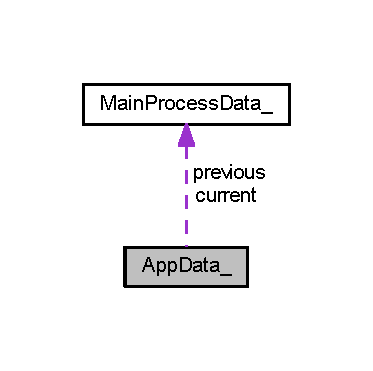
\includegraphics[width=179pt]{struct_app_data____coll__graph}
\end{center}
\end{figure}
\subsection*{Data Fields}
\begin{DoxyCompactItemize}
\item 
\mbox{\hyperlink{main_8c_a10c0332e7cd68abe97ec61fa4ac93383}{Main\+Process\+Data}} \mbox{\hyperlink{struct_app_data___aab83920d96d162d986df2bbce5d382ab}{current}}
\item 
\mbox{\hyperlink{main_8c_a10c0332e7cd68abe97ec61fa4ac93383}{Main\+Process\+Data}} \mbox{\hyperlink{struct_app_data___a57a5b5fd3e09c0d8651bffc358acd3c4}{previous}}
\end{DoxyCompactItemize}


\subsection{Detailed Description}


Definition at line 97 of file main.\+c.



\subsection{Field Documentation}
\mbox{\Hypertarget{struct_app_data___aab83920d96d162d986df2bbce5d382ab}\label{struct_app_data___aab83920d96d162d986df2bbce5d382ab}} 
\index{App\+Data\+\_\+@{App\+Data\+\_\+}!current@{current}}
\index{current@{current}!App\+Data\+\_\+@{App\+Data\+\_\+}}
\subsubsection{\texorpdfstring{current}{current}}
{\footnotesize\ttfamily \mbox{\hyperlink{main_8c_a10c0332e7cd68abe97ec61fa4ac93383}{Main\+Process\+Data}} current}



Definition at line 98 of file main.\+c.

\mbox{\Hypertarget{struct_app_data___a57a5b5fd3e09c0d8651bffc358acd3c4}\label{struct_app_data___a57a5b5fd3e09c0d8651bffc358acd3c4}} 
\index{App\+Data\+\_\+@{App\+Data\+\_\+}!previous@{previous}}
\index{previous@{previous}!App\+Data\+\_\+@{App\+Data\+\_\+}}
\subsubsection{\texorpdfstring{previous}{previous}}
{\footnotesize\ttfamily \mbox{\hyperlink{main_8c_a10c0332e7cd68abe97ec61fa4ac93383}{Main\+Process\+Data}} previous}



Definition at line 99 of file main.\+c.



The documentation for this struct was generated from the following file\+:\begin{DoxyCompactItemize}
\item 
\mbox{\hyperlink{main_8c}{main.\+c}}\end{DoxyCompactItemize}

\hypertarget{struct_main_process_data__}{}\section{Main\+Process\+Data\+\_\+ Struct Reference}
\label{struct_main_process_data__}\index{Main\+Process\+Data\+\_\+@{Main\+Process\+Data\+\_\+}}
\subsection*{Data Fields}
\begin{DoxyCompactItemize}
\item 
char \mbox{\hyperlink{struct_main_process_data___ae9a120d1fe4b71425af49710ed6c7a03}{buf\+Info}} \mbox{[}20\mbox{]}
\item 
double \mbox{\hyperlink{struct_main_process_data___a79b8e036dca6911e3295a47d99f21f43}{distance}}
\item 
float \mbox{\hyperlink{struct_main_process_data___a19546b530c18a3d4bba8eafbb4778f69}{Heart\+Rate}}
\end{DoxyCompactItemize}


\subsection{Detailed Description}


Definition at line 82 of file main.\+c.



\subsection{Field Documentation}
\mbox{\Hypertarget{struct_main_process_data___ae9a120d1fe4b71425af49710ed6c7a03}\label{struct_main_process_data___ae9a120d1fe4b71425af49710ed6c7a03}} 
\index{Main\+Process\+Data\+\_\+@{Main\+Process\+Data\+\_\+}!buf\+Info@{buf\+Info}}
\index{buf\+Info@{buf\+Info}!Main\+Process\+Data\+\_\+@{Main\+Process\+Data\+\_\+}}
\subsubsection{\texorpdfstring{buf\+Info}{bufInfo}}
{\footnotesize\ttfamily char buf\+Info\mbox{[}20\mbox{]}}



Definition at line 84 of file main.\+c.

\mbox{\Hypertarget{struct_main_process_data___a79b8e036dca6911e3295a47d99f21f43}\label{struct_main_process_data___a79b8e036dca6911e3295a47d99f21f43}} 
\index{Main\+Process\+Data\+\_\+@{Main\+Process\+Data\+\_\+}!distance@{distance}}
\index{distance@{distance}!Main\+Process\+Data\+\_\+@{Main\+Process\+Data\+\_\+}}
\subsubsection{\texorpdfstring{distance}{distance}}
{\footnotesize\ttfamily double distance}



Definition at line 85 of file main.\+c.

\mbox{\Hypertarget{struct_main_process_data___a19546b530c18a3d4bba8eafbb4778f69}\label{struct_main_process_data___a19546b530c18a3d4bba8eafbb4778f69}} 
\index{Main\+Process\+Data\+\_\+@{Main\+Process\+Data\+\_\+}!Heart\+Rate@{Heart\+Rate}}
\index{Heart\+Rate@{Heart\+Rate}!Main\+Process\+Data\+\_\+@{Main\+Process\+Data\+\_\+}}
\subsubsection{\texorpdfstring{Heart\+Rate}{HeartRate}}
{\footnotesize\ttfamily float Heart\+Rate}



Definition at line 86 of file main.\+c.



The documentation for this struct was generated from the following file\+:\begin{DoxyCompactItemize}
\item 
Src/\mbox{\hyperlink{main_8c}{main.\+c}}\end{DoxyCompactItemize}

\chapter{File Documentation}
\hypertarget{adc_8c}{}\section{Src/adc.c File Reference}
\label{adc_8c}\index{Src/adc.\+c@{Src/adc.\+c}}
{\ttfamily \#include \char`\"{}adc.\+h\char`\"{}}\newline
{\ttfamily \#include \char`\"{}gpio.\+h\char`\"{}}\newline
Include dependency graph for adc.\+c\+:\nopagebreak
\begin{figure}[H]
\begin{center}
\leavevmode
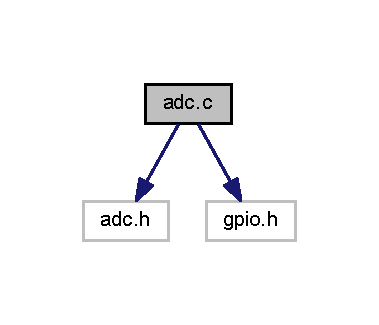
\includegraphics[width=182pt]{adc_8c__incl}
\end{center}
\end{figure}
\subsection*{Functions}
\begin{DoxyCompactItemize}
\item 
void \mbox{\hyperlink{adc_8c_acccd58aa70215a6b184ad242312ffd0c}{M\+X\+\_\+\+A\+D\+C1\+\_\+\+Init}} (void)
\item 
void \mbox{\hyperlink{adc_8c_a101e2e3433dfe72bbbd0ae3a84489263}{M\+X\+\_\+\+A\+D\+C2\+\_\+\+Init}} (void)
\item 
void \mbox{\hyperlink{adc_8c_ac3139540667c403c5dfd37a99c610b1c}{H\+A\+L\+\_\+\+A\+D\+C\+\_\+\+Msp\+Init}} (A\+D\+C\+\_\+\+Handle\+Type\+Def $\ast$adc\+Handle)
\item 
void \mbox{\hyperlink{adc_8c_a3f61f2c2af0f122f81a87af8ad7b4360}{H\+A\+L\+\_\+\+A\+D\+C\+\_\+\+Msp\+De\+Init}} (A\+D\+C\+\_\+\+Handle\+Type\+Def $\ast$adc\+Handle)
\end{DoxyCompactItemize}
\subsection*{Variables}
\begin{DoxyCompactItemize}
\item 
A\+D\+C\+\_\+\+Handle\+Type\+Def \mbox{\hyperlink{adc_8c_a22b804736f5648d52f639b2647d4ed13}{hadc1}}
\item 
A\+D\+C\+\_\+\+Handle\+Type\+Def \mbox{\hyperlink{adc_8c_acd9221f1aa19aebfe0b744947f2daf49}{hadc2}}
\end{DoxyCompactItemize}


\subsection{Function Documentation}
\mbox{\Hypertarget{adc_8c_a3f61f2c2af0f122f81a87af8ad7b4360}\label{adc_8c_a3f61f2c2af0f122f81a87af8ad7b4360}} 
\index{adc.\+c@{adc.\+c}!H\+A\+L\+\_\+\+A\+D\+C\+\_\+\+Msp\+De\+Init@{H\+A\+L\+\_\+\+A\+D\+C\+\_\+\+Msp\+De\+Init}}
\index{H\+A\+L\+\_\+\+A\+D\+C\+\_\+\+Msp\+De\+Init@{H\+A\+L\+\_\+\+A\+D\+C\+\_\+\+Msp\+De\+Init}!adc.\+c@{adc.\+c}}
\subsubsection{\texorpdfstring{H\+A\+L\+\_\+\+A\+D\+C\+\_\+\+Msp\+De\+Init()}{HAL\_ADC\_MspDeInit()}}
{\footnotesize\ttfamily void H\+A\+L\+\_\+\+A\+D\+C\+\_\+\+Msp\+De\+Init (\begin{DoxyParamCaption}\item[{A\+D\+C\+\_\+\+Handle\+Type\+Def $\ast$}]{adc\+Handle }\end{DoxyParamCaption})}

A\+D\+C1 G\+P\+IO Configuration ~\newline
~\newline
~\newline
~\newline
P\+B1 ------$>$ A\+D\+C1\+\_\+\+I\+N9

Uncomment the line below to disable the \char`\"{}\+A\+D\+C\+\_\+\+I\+R\+Qn\char`\"{} interrupt Be aware, disabling shared interrupt may affect other I\+Ps

A\+D\+C2 G\+P\+IO Configuration ~\newline
~\newline
P\+A1 ------$>$ A\+D\+C2\+\_\+\+I\+N1

Uncomment the line below to disable the \char`\"{}\+A\+D\+C\+\_\+\+I\+R\+Qn\char`\"{} interrupt Be aware, disabling shared interrupt may affect other I\+Ps

Definition at line 185 of file adc.\+c.

\mbox{\Hypertarget{adc_8c_ac3139540667c403c5dfd37a99c610b1c}\label{adc_8c_ac3139540667c403c5dfd37a99c610b1c}} 
\index{adc.\+c@{adc.\+c}!H\+A\+L\+\_\+\+A\+D\+C\+\_\+\+Msp\+Init@{H\+A\+L\+\_\+\+A\+D\+C\+\_\+\+Msp\+Init}}
\index{H\+A\+L\+\_\+\+A\+D\+C\+\_\+\+Msp\+Init@{H\+A\+L\+\_\+\+A\+D\+C\+\_\+\+Msp\+Init}!adc.\+c@{adc.\+c}}
\subsubsection{\texorpdfstring{H\+A\+L\+\_\+\+A\+D\+C\+\_\+\+Msp\+Init()}{HAL\_ADC\_MspInit()}}
{\footnotesize\ttfamily void H\+A\+L\+\_\+\+A\+D\+C\+\_\+\+Msp\+Init (\begin{DoxyParamCaption}\item[{A\+D\+C\+\_\+\+Handle\+Type\+Def $\ast$}]{adc\+Handle }\end{DoxyParamCaption})}

A\+D\+C1 G\+P\+IO Configuration ~\newline
~\newline
P\+B1 ------$>$ A\+D\+C1\+\_\+\+I\+N9

A\+D\+C2 G\+P\+IO Configuration ~\newline
P\+A1 -\/-\/-\/---$>$ A\+D\+C2\+\_\+\+I\+N1

Definition at line 133 of file adc.\+c.

\mbox{\Hypertarget{adc_8c_acccd58aa70215a6b184ad242312ffd0c}\label{adc_8c_acccd58aa70215a6b184ad242312ffd0c}} 
\index{adc.\+c@{adc.\+c}!M\+X\+\_\+\+A\+D\+C1\+\_\+\+Init@{M\+X\+\_\+\+A\+D\+C1\+\_\+\+Init}}
\index{M\+X\+\_\+\+A\+D\+C1\+\_\+\+Init@{M\+X\+\_\+\+A\+D\+C1\+\_\+\+Init}!adc.\+c@{adc.\+c}}
\subsubsection{\texorpdfstring{M\+X\+\_\+\+A\+D\+C1\+\_\+\+Init()}{MX\_ADC1\_Init()}}
{\footnotesize\ttfamily void M\+X\+\_\+\+A\+D\+C1\+\_\+\+Init (\begin{DoxyParamCaption}\item[{void}]{ }\end{DoxyParamCaption})}

Configure the global features of the A\+DC (Clock, Resolution, Data Alignment and number of conversion)

Configure for the selected A\+DC regular channel its corresponding rank in the sequencer and its sample time.

Definition at line 63 of file adc.\+c.

Here is the call graph for this function\+:\nopagebreak
\begin{figure}[H]
\begin{center}
\leavevmode
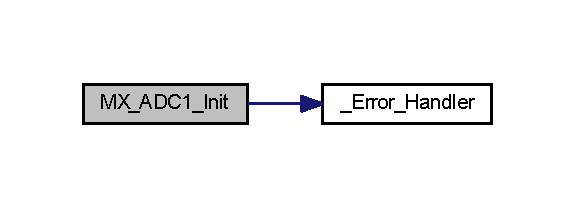
\includegraphics[width=276pt]{adc_8c_acccd58aa70215a6b184ad242312ffd0c_cgraph}
\end{center}
\end{figure}
Here is the caller graph for this function\+:\nopagebreak
\begin{figure}[H]
\begin{center}
\leavevmode
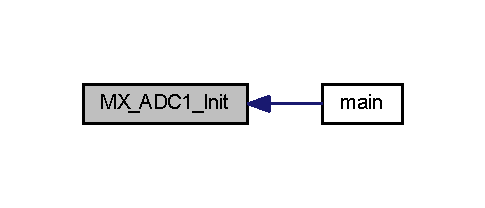
\includegraphics[width=233pt]{adc_8c_acccd58aa70215a6b184ad242312ffd0c_icgraph}
\end{center}
\end{figure}
\mbox{\Hypertarget{adc_8c_a101e2e3433dfe72bbbd0ae3a84489263}\label{adc_8c_a101e2e3433dfe72bbbd0ae3a84489263}} 
\index{adc.\+c@{adc.\+c}!M\+X\+\_\+\+A\+D\+C2\+\_\+\+Init@{M\+X\+\_\+\+A\+D\+C2\+\_\+\+Init}}
\index{M\+X\+\_\+\+A\+D\+C2\+\_\+\+Init@{M\+X\+\_\+\+A\+D\+C2\+\_\+\+Init}!adc.\+c@{adc.\+c}}
\subsubsection{\texorpdfstring{M\+X\+\_\+\+A\+D\+C2\+\_\+\+Init()}{MX\_ADC2\_Init()}}
{\footnotesize\ttfamily void M\+X\+\_\+\+A\+D\+C2\+\_\+\+Init (\begin{DoxyParamCaption}\item[{void}]{ }\end{DoxyParamCaption})}

Configure the global features of the A\+DC (Clock, Resolution, Data Alignment and number of conversion)

Configure for the selected A\+DC regular channel its corresponding rank in the sequencer and its sample time.

Definition at line 98 of file adc.\+c.

Here is the call graph for this function\+:\nopagebreak
\begin{figure}[H]
\begin{center}
\leavevmode
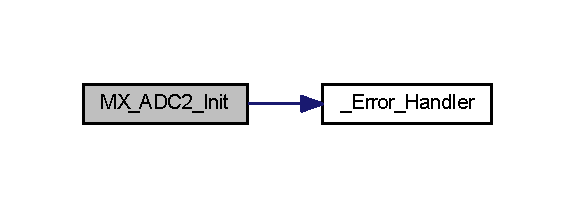
\includegraphics[width=276pt]{adc_8c_a101e2e3433dfe72bbbd0ae3a84489263_cgraph}
\end{center}
\end{figure}
Here is the caller graph for this function\+:\nopagebreak
\begin{figure}[H]
\begin{center}
\leavevmode
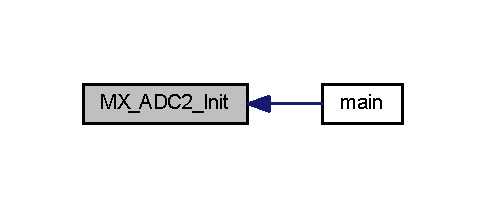
\includegraphics[width=233pt]{adc_8c_a101e2e3433dfe72bbbd0ae3a84489263_icgraph}
\end{center}
\end{figure}


\subsection{Variable Documentation}
\mbox{\Hypertarget{adc_8c_a22b804736f5648d52f639b2647d4ed13}\label{adc_8c_a22b804736f5648d52f639b2647d4ed13}} 
\index{adc.\+c@{adc.\+c}!hadc1@{hadc1}}
\index{hadc1@{hadc1}!adc.\+c@{adc.\+c}}
\subsubsection{\texorpdfstring{hadc1}{hadc1}}
{\footnotesize\ttfamily A\+D\+C\+\_\+\+Handle\+Type\+Def hadc1}

File Name \+: \mbox{\hyperlink{adc_8c}{A\+D\+C.\+c}} Description \+: This file provides code for the configuration of the A\+DC instances.

This notice applies to any and all portions of this file that are not between comment pairs U\+S\+ER C\+O\+DE B\+E\+G\+IN and U\+S\+ER C\+O\+DE E\+ND. Other portions of this file, whether inserted by the user or by software development tools are owned by their respective copyright owners.

Copyright (c) 2018 S\+T\+Microelectronics International N.\+V. All rights reserved.

Redistribution and use in source and binary forms, with or without modification, are permitted, provided that the following conditions are met\+:


\begin{DoxyEnumerate}
\item Redistribution of source code must retain the above copyright notice, this list of conditions and the following disclaimer.
\item Redistributions in binary form must reproduce the above copyright notice, this list of conditions and the following disclaimer in the documentation and/or other materials provided with the distribution.
\item Neither the name of S\+T\+Microelectronics nor the names of other contributors to this software may be used to endorse or promote products derived from this software without specific written permission.
\item This software, including modifications and/or derivative works of this software, must execute solely and exclusively on microcontroller or microprocessor devices manufactured by or for S\+T\+Microelectronics.
\item Redistribution and use of this software other than as permitted under this license is void and will automatically terminate your rights under this license.
\end{DoxyEnumerate}

T\+H\+IS S\+O\+F\+T\+W\+A\+RE IS P\+R\+O\+V\+I\+D\+ED BY S\+T\+M\+I\+C\+R\+O\+E\+L\+E\+C\+T\+R\+O\+N\+I\+CS A\+ND C\+O\+N\+T\+R\+I\+B\+U\+T\+O\+RS \char`\"{}\+A\+S I\+S\char`\"{} A\+ND A\+NY E\+X\+P\+R\+E\+SS, I\+M\+P\+L\+I\+ED OR S\+T\+A\+T\+U\+T\+O\+RY W\+A\+R\+R\+A\+N\+T\+I\+ES, I\+N\+C\+L\+U\+D\+I\+NG, B\+UT N\+OT L\+I\+M\+I\+T\+ED TO, T\+HE I\+M\+P\+L\+I\+ED W\+A\+R\+R\+A\+N\+T\+I\+ES OF M\+E\+R\+C\+H\+A\+N\+T\+A\+B\+I\+L\+I\+TY, F\+I\+T\+N\+E\+SS F\+OR A P\+A\+R\+T\+I\+C\+U\+L\+AR P\+U\+R\+P\+O\+SE A\+ND N\+O\+N-\/\+I\+N\+F\+R\+I\+N\+G\+E\+M\+E\+NT OF T\+H\+I\+RD P\+A\+R\+TY I\+N\+T\+E\+L\+L\+E\+C\+T\+U\+AL P\+R\+O\+P\+E\+R\+TY R\+I\+G\+H\+TS A\+RE D\+I\+S\+C\+L\+A\+I\+M\+ED TO T\+HE F\+U\+L\+L\+E\+ST E\+X\+T\+E\+NT P\+E\+R\+M\+I\+T\+T\+ED BY L\+AW. IN NO E\+V\+E\+NT S\+H\+A\+LL S\+T\+M\+I\+C\+R\+O\+E\+L\+E\+C\+T\+R\+O\+N\+I\+CS OR C\+O\+N\+T\+R\+I\+B\+U\+T\+O\+RS BE L\+I\+A\+B\+LE F\+OR A\+NY D\+I\+R\+E\+CT, I\+N\+D\+I\+R\+E\+CT, I\+N\+C\+I\+D\+E\+N\+T\+AL, S\+P\+E\+C\+I\+AL, E\+X\+E\+M\+P\+L\+A\+RY, OR C\+O\+N\+S\+E\+Q\+U\+E\+N\+T\+I\+AL D\+A\+M\+A\+G\+ES (I\+N\+C\+L\+U\+D\+I\+NG, B\+UT N\+OT L\+I\+M\+I\+T\+ED TO, P\+R\+O\+C\+U\+R\+E\+M\+E\+NT OF S\+U\+B\+S\+T\+I\+T\+U\+TE G\+O\+O\+DS OR S\+E\+R\+V\+I\+C\+ES; L\+O\+SS OF U\+SE, D\+A\+TA, OR P\+R\+O\+F\+I\+TS; OR B\+U\+S\+I\+N\+E\+SS I\+N\+T\+E\+R\+R\+U\+P\+T\+I\+ON) H\+O\+W\+E\+V\+ER C\+A\+U\+S\+ED A\+ND ON A\+NY T\+H\+E\+O\+RY OF L\+I\+A\+B\+I\+L\+I\+TY, W\+H\+E\+T\+H\+ER IN C\+O\+N\+T\+R\+A\+CT, S\+T\+R\+I\+CT L\+I\+A\+B\+I\+L\+I\+TY, OR T\+O\+RT (I\+N\+C\+L\+U\+D\+I\+NG N\+E\+G\+L\+I\+G\+E\+N\+CE OR O\+T\+H\+E\+R\+W\+I\+SE) A\+R\+I\+S\+I\+NG IN A\+NY W\+AY O\+UT OF T\+HE U\+SE OF T\+H\+IS S\+O\+F\+T\+W\+A\+RE, E\+V\+EN IF A\+D\+V\+I\+S\+ED OF T\+HE P\+O\+S\+S\+I\+B\+I\+L\+I\+TY OF S\+U\+CH D\+A\+M\+A\+GE. 

Definition at line 59 of file adc.\+c.

\mbox{\Hypertarget{adc_8c_acd9221f1aa19aebfe0b744947f2daf49}\label{adc_8c_acd9221f1aa19aebfe0b744947f2daf49}} 
\index{adc.\+c@{adc.\+c}!hadc2@{hadc2}}
\index{hadc2@{hadc2}!adc.\+c@{adc.\+c}}
\subsubsection{\texorpdfstring{hadc2}{hadc2}}
{\footnotesize\ttfamily A\+D\+C\+\_\+\+Handle\+Type\+Def hadc2}



Definition at line 60 of file adc.\+c.


\hypertarget{dma_8c}{}\section{dma.\+c File Reference}
\label{dma_8c}\index{dma.\+c@{dma.\+c}}
{\ttfamily \#include \char`\"{}dma.\+h\char`\"{}}\newline
Include dependency graph for dma.\+c\+:
\nopagebreak
\begin{figure}[H]
\begin{center}
\leavevmode
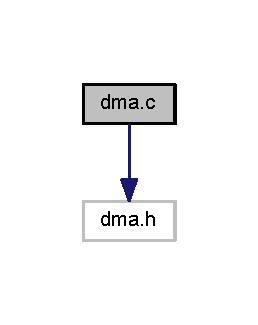
\includegraphics[width=124pt]{dma_8c__incl}
\end{center}
\end{figure}
\subsection*{Functions}
\begin{DoxyCompactItemize}
\item 
void \mbox{\hyperlink{dma_8c_a323249dac769f9855c10b4ec9446b707}{M\+X\+\_\+\+D\+M\+A\+\_\+\+Init}} (void)
\end{DoxyCompactItemize}


\subsection{Function Documentation}
\mbox{\Hypertarget{dma_8c_a323249dac769f9855c10b4ec9446b707}\label{dma_8c_a323249dac769f9855c10b4ec9446b707}} 
\index{dma.\+c@{dma.\+c}!M\+X\+\_\+\+D\+M\+A\+\_\+\+Init@{M\+X\+\_\+\+D\+M\+A\+\_\+\+Init}}
\index{M\+X\+\_\+\+D\+M\+A\+\_\+\+Init@{M\+X\+\_\+\+D\+M\+A\+\_\+\+Init}!dma.\+c@{dma.\+c}}
\subsubsection{\texorpdfstring{M\+X\+\_\+\+D\+M\+A\+\_\+\+Init()}{MX\_DMA\_Init()}}
{\footnotesize\ttfamily void M\+X\+\_\+\+D\+M\+A\+\_\+\+Init (\begin{DoxyParamCaption}\item[{void}]{ }\end{DoxyParamCaption})}

File Name \+: \mbox{\hyperlink{dma_8c}{dma.\+c}} Description \+: This file provides code for the configuration of all the requested memory to memory D\+MA transfers.

This notice applies to any and all portions of this file that are not between comment pairs U\+S\+ER C\+O\+DE B\+E\+G\+IN and U\+S\+ER C\+O\+DE E\+ND. Other portions of this file, whether inserted by the user or by software development tools are owned by their respective copyright owners.

Copyright (c) 2018 S\+T\+Microelectronics International N.\+V. All rights reserved.

Redistribution and use in source and binary forms, with or without modification, are permitted, provided that the following conditions are met\+:


\begin{DoxyEnumerate}
\item Redistribution of source code must retain the above copyright notice, this list of conditions and the following disclaimer.
\item Redistributions in binary form must reproduce the above copyright notice, this list of conditions and the following disclaimer in the documentation and/or other materials provided with the distribution.
\item Neither the name of S\+T\+Microelectronics nor the names of other contributors to this software may be used to endorse or promote products derived from this software without specific written permission.
\item This software, including modifications and/or derivative works of this software, must execute solely and exclusively on microcontroller or microprocessor devices manufactured by or for S\+T\+Microelectronics.
\item Redistribution and use of this software other than as permitted under this license is void and will automatically terminate your rights under this license.
\end{DoxyEnumerate}

T\+H\+IS S\+O\+F\+T\+W\+A\+RE IS P\+R\+O\+V\+I\+D\+ED BY S\+T\+M\+I\+C\+R\+O\+E\+L\+E\+C\+T\+R\+O\+N\+I\+CS A\+ND C\+O\+N\+T\+R\+I\+B\+U\+T\+O\+RS \char`\"{}\+A\+S I\+S\char`\"{} A\+ND A\+NY E\+X\+P\+R\+E\+SS, I\+M\+P\+L\+I\+ED OR S\+T\+A\+T\+U\+T\+O\+RY W\+A\+R\+R\+A\+N\+T\+I\+ES, I\+N\+C\+L\+U\+D\+I\+NG, B\+UT N\+OT L\+I\+M\+I\+T\+ED TO, T\+HE I\+M\+P\+L\+I\+ED W\+A\+R\+R\+A\+N\+T\+I\+ES OF M\+E\+R\+C\+H\+A\+N\+T\+A\+B\+I\+L\+I\+TY, F\+I\+T\+N\+E\+SS F\+OR A P\+A\+R\+T\+I\+C\+U\+L\+AR P\+U\+R\+P\+O\+SE A\+ND N\+O\+N-\/\+I\+N\+F\+R\+I\+N\+G\+E\+M\+E\+NT OF T\+H\+I\+RD P\+A\+R\+TY I\+N\+T\+E\+L\+L\+E\+C\+T\+U\+AL P\+R\+O\+P\+E\+R\+TY R\+I\+G\+H\+TS A\+RE D\+I\+S\+C\+L\+A\+I\+M\+ED TO T\+HE F\+U\+L\+L\+E\+ST E\+X\+T\+E\+NT P\+E\+R\+M\+I\+T\+T\+ED BY L\+AW. IN NO E\+V\+E\+NT S\+H\+A\+LL S\+T\+M\+I\+C\+R\+O\+E\+L\+E\+C\+T\+R\+O\+N\+I\+CS OR C\+O\+N\+T\+R\+I\+B\+U\+T\+O\+RS BE L\+I\+A\+B\+LE F\+OR A\+NY D\+I\+R\+E\+CT, I\+N\+D\+I\+R\+E\+CT, I\+N\+C\+I\+D\+E\+N\+T\+AL, S\+P\+E\+C\+I\+AL, E\+X\+E\+M\+P\+L\+A\+RY, OR C\+O\+N\+S\+E\+Q\+U\+E\+N\+T\+I\+AL D\+A\+M\+A\+G\+ES (I\+N\+C\+L\+U\+D\+I\+NG, B\+UT N\+OT L\+I\+M\+I\+T\+ED TO, P\+R\+O\+C\+U\+R\+E\+M\+E\+NT OF S\+U\+B\+S\+T\+I\+T\+U\+TE G\+O\+O\+DS OR S\+E\+R\+V\+I\+C\+ES; L\+O\+SS OF U\+SE, D\+A\+TA, OR P\+R\+O\+F\+I\+TS; OR B\+U\+S\+I\+N\+E\+SS I\+N\+T\+E\+R\+R\+U\+P\+T\+I\+ON) H\+O\+W\+E\+V\+ER C\+A\+U\+S\+ED A\+ND ON A\+NY T\+H\+E\+O\+RY OF L\+I\+A\+B\+I\+L\+I\+TY, W\+H\+E\+T\+H\+ER IN C\+O\+N\+T\+R\+A\+CT, S\+T\+R\+I\+CT L\+I\+A\+B\+I\+L\+I\+TY, OR T\+O\+RT (I\+N\+C\+L\+U\+D\+I\+NG N\+E\+G\+L\+I\+G\+E\+N\+CE OR O\+T\+H\+E\+R\+W\+I\+SE) A\+R\+I\+S\+I\+NG IN A\+NY W\+AY O\+UT OF T\+HE U\+SE OF T\+H\+IS S\+O\+F\+T\+W\+A\+RE, E\+V\+EN IF A\+D\+V\+I\+S\+ED OF T\+HE P\+O\+S\+S\+I\+B\+I\+L\+I\+TY OF S\+U\+CH D\+A\+M\+A\+GE. Enable D\+MA controller clock 

Definition at line 67 of file dma.\+c.

Here is the caller graph for this function\+:
\nopagebreak
\begin{figure}[H]
\begin{center}
\leavevmode
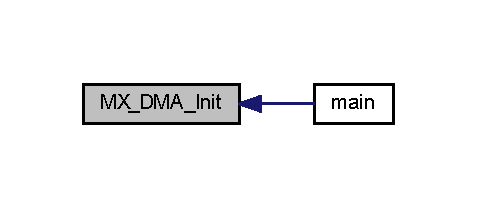
\includegraphics[width=229pt]{dma_8c_a323249dac769f9855c10b4ec9446b707_icgraph}
\end{center}
\end{figure}

\hypertarget{fatfs_8c}{}\section{Src/fatfs.c File Reference}
\label{fatfs_8c}\index{Src/fatfs.\+c@{Src/fatfs.\+c}}


Code for fatfs applications.  


{\ttfamily \#include \char`\"{}fatfs.\+h\char`\"{}}\newline
Include dependency graph for fatfs.\+c\+:\nopagebreak
\begin{figure}[H]
\begin{center}
\leavevmode
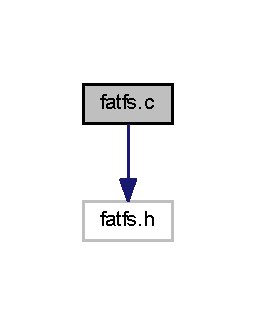
\includegraphics[width=288pt]{fatfs_8c__incl}
\end{center}
\end{figure}
\subsection*{Functions}
\begin{DoxyCompactItemize}
\item 
void \mbox{\hyperlink{fatfs_8c_a3712bd1d3043334cf9343acc30bd2604}{M\+X\+\_\+\+F\+A\+T\+F\+S\+\_\+\+Init}} (void)
\item 
D\+W\+O\+RD \mbox{\hyperlink{fatfs_8c_af58b536abfd30f77213f4ecaf2ac52f5}{get\+\_\+fattime}} (void)
\begin{DoxyCompactList}\small\item\em Gets Time from R\+TC. \end{DoxyCompactList}\end{DoxyCompactItemize}
\subsection*{Variables}
\begin{DoxyCompactItemize}
\item 
uint8\+\_\+t \mbox{\hyperlink{fatfs_8c_a424889af713d1b8afbb3e02352924792}{ret\+U\+S\+ER}}
\item 
char \mbox{\hyperlink{fatfs_8c_aba9c3aa07bcf2804dedcc0f7014a78ba}{U\+S\+E\+R\+Path}} \mbox{[}4\mbox{]}
\item 
F\+A\+T\+FS \mbox{\hyperlink{fatfs_8c_aeb1982f45f4eaf65071f64491c3c2c2f}{U\+S\+E\+R\+Fat\+FS}}
\item 
F\+IL \mbox{\hyperlink{fatfs_8c_a4e242af5cb4d75dbcb96a3213a3b1401}{U\+S\+E\+R\+File}}
\end{DoxyCompactItemize}


\subsection{Detailed Description}
Code for fatfs applications. 

This notice applies to any and all portions of this file that are not between comment pairs U\+S\+ER C\+O\+DE B\+E\+G\+IN and U\+S\+ER C\+O\+DE E\+ND. Other portions of this file, whether inserted by the user or by software development tools are owned by their respective copyright owners.

Copyright (c) 2018 S\+T\+Microelectronics International N.\+V. All rights reserved.

Redistribution and use in source and binary forms, with or without modification, are permitted, provided that the following conditions are met\+:


\begin{DoxyEnumerate}
\item Redistribution of source code must retain the above copyright notice, this list of conditions and the following disclaimer.
\item Redistributions in binary form must reproduce the above copyright notice, this list of conditions and the following disclaimer in the documentation and/or other materials provided with the distribution.
\item Neither the name of S\+T\+Microelectronics nor the names of other contributors to this software may be used to endorse or promote products derived from this software without specific written permission.
\item This software, including modifications and/or derivative works of this software, must execute solely and exclusively on microcontroller or microprocessor devices manufactured by or for S\+T\+Microelectronics.
\item Redistribution and use of this software other than as permitted under this license is void and will automatically terminate your rights under this license.
\end{DoxyEnumerate}

T\+H\+IS S\+O\+F\+T\+W\+A\+RE IS P\+R\+O\+V\+I\+D\+ED BY S\+T\+M\+I\+C\+R\+O\+E\+L\+E\+C\+T\+R\+O\+N\+I\+CS A\+ND C\+O\+N\+T\+R\+I\+B\+U\+T\+O\+RS \char`\"{}\+A\+S I\+S\char`\"{} A\+ND A\+NY E\+X\+P\+R\+E\+SS, I\+M\+P\+L\+I\+ED OR S\+T\+A\+T\+U\+T\+O\+RY W\+A\+R\+R\+A\+N\+T\+I\+ES, I\+N\+C\+L\+U\+D\+I\+NG, B\+UT N\+OT L\+I\+M\+I\+T\+ED TO, T\+HE I\+M\+P\+L\+I\+ED W\+A\+R\+R\+A\+N\+T\+I\+ES OF M\+E\+R\+C\+H\+A\+N\+T\+A\+B\+I\+L\+I\+TY, F\+I\+T\+N\+E\+SS F\+OR A P\+A\+R\+T\+I\+C\+U\+L\+AR P\+U\+R\+P\+O\+SE A\+ND N\+O\+N-\/\+I\+N\+F\+R\+I\+N\+G\+E\+M\+E\+NT OF T\+H\+I\+RD P\+A\+R\+TY I\+N\+T\+E\+L\+L\+E\+C\+T\+U\+AL P\+R\+O\+P\+E\+R\+TY R\+I\+G\+H\+TS A\+RE D\+I\+S\+C\+L\+A\+I\+M\+ED TO T\+HE F\+U\+L\+L\+E\+ST E\+X\+T\+E\+NT P\+E\+R\+M\+I\+T\+T\+ED BY L\+AW. IN NO E\+V\+E\+NT S\+H\+A\+LL S\+T\+M\+I\+C\+R\+O\+E\+L\+E\+C\+T\+R\+O\+N\+I\+CS OR C\+O\+N\+T\+R\+I\+B\+U\+T\+O\+RS BE L\+I\+A\+B\+LE F\+OR A\+NY D\+I\+R\+E\+CT, I\+N\+D\+I\+R\+E\+CT, I\+N\+C\+I\+D\+E\+N\+T\+AL, S\+P\+E\+C\+I\+AL, E\+X\+E\+M\+P\+L\+A\+RY, OR C\+O\+N\+S\+E\+Q\+U\+E\+N\+T\+I\+AL D\+A\+M\+A\+G\+ES (I\+N\+C\+L\+U\+D\+I\+NG, B\+UT N\+OT L\+I\+M\+I\+T\+ED TO, P\+R\+O\+C\+U\+R\+E\+M\+E\+NT OF S\+U\+B\+S\+T\+I\+T\+U\+TE G\+O\+O\+DS OR S\+E\+R\+V\+I\+C\+ES; L\+O\+SS OF U\+SE, D\+A\+TA, OR P\+R\+O\+F\+I\+TS; OR B\+U\+S\+I\+N\+E\+SS I\+N\+T\+E\+R\+R\+U\+P\+T\+I\+ON) H\+O\+W\+E\+V\+ER C\+A\+U\+S\+ED A\+ND ON A\+NY T\+H\+E\+O\+RY OF L\+I\+A\+B\+I\+L\+I\+TY, W\+H\+E\+T\+H\+ER IN C\+O\+N\+T\+R\+A\+CT, S\+T\+R\+I\+CT L\+I\+A\+B\+I\+L\+I\+TY, OR T\+O\+RT (I\+N\+C\+L\+U\+D\+I\+NG N\+E\+G\+L\+I\+G\+E\+N\+CE OR O\+T\+H\+E\+R\+W\+I\+SE) A\+R\+I\+S\+I\+NG IN A\+NY W\+AY O\+UT OF T\+HE U\+SE OF T\+H\+IS S\+O\+F\+T\+W\+A\+RE, E\+V\+EN IF A\+D\+V\+I\+S\+ED OF T\+HE P\+O\+S\+S\+I\+B\+I\+L\+I\+TY OF S\+U\+CH D\+A\+M\+A\+GE. 

\subsection{Function Documentation}
\mbox{\Hypertarget{fatfs_8c_af58b536abfd30f77213f4ecaf2ac52f5}\label{fatfs_8c_af58b536abfd30f77213f4ecaf2ac52f5}} 
\index{fatfs.\+c@{fatfs.\+c}!get\+\_\+fattime@{get\+\_\+fattime}}
\index{get\+\_\+fattime@{get\+\_\+fattime}!fatfs.\+c@{fatfs.\+c}}
\subsubsection{\texorpdfstring{get\+\_\+fattime()}{get\_fattime()}}
{\footnotesize\ttfamily D\+W\+O\+RD get\+\_\+fattime (\begin{DoxyParamCaption}\item[{void}]{ }\end{DoxyParamCaption})}



Gets Time from R\+TC. 


\begin{DoxyParams}{Parameters}
{\em None} & \\
\hline
\end{DoxyParams}

\begin{DoxyRetVals}{Return values}
{\em Time} & in D\+W\+O\+RD \\
\hline
\end{DoxyRetVals}


Definition at line 75 of file fatfs.\+c.

\mbox{\Hypertarget{fatfs_8c_a3712bd1d3043334cf9343acc30bd2604}\label{fatfs_8c_a3712bd1d3043334cf9343acc30bd2604}} 
\index{fatfs.\+c@{fatfs.\+c}!M\+X\+\_\+\+F\+A\+T\+F\+S\+\_\+\+Init@{M\+X\+\_\+\+F\+A\+T\+F\+S\+\_\+\+Init}}
\index{M\+X\+\_\+\+F\+A\+T\+F\+S\+\_\+\+Init@{M\+X\+\_\+\+F\+A\+T\+F\+S\+\_\+\+Init}!fatfs.\+c@{fatfs.\+c}}
\subsubsection{\texorpdfstring{M\+X\+\_\+\+F\+A\+T\+F\+S\+\_\+\+Init()}{MX\_FATFS\_Init()}}
{\footnotesize\ttfamily void M\+X\+\_\+\+F\+A\+T\+F\+S\+\_\+\+Init (\begin{DoxyParamCaption}\item[{void}]{ }\end{DoxyParamCaption})}



Definition at line 60 of file fatfs.\+c.

Here is the caller graph for this function\+:\nopagebreak
\begin{figure}[H]
\begin{center}
\leavevmode
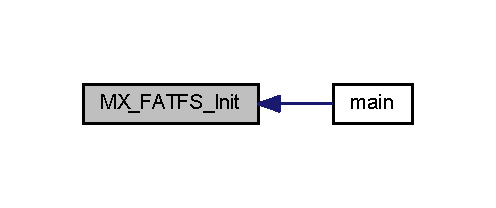
\includegraphics[width=238pt]{fatfs_8c_a3712bd1d3043334cf9343acc30bd2604_icgraph}
\end{center}
\end{figure}


\subsection{Variable Documentation}
\mbox{\Hypertarget{fatfs_8c_a424889af713d1b8afbb3e02352924792}\label{fatfs_8c_a424889af713d1b8afbb3e02352924792}} 
\index{fatfs.\+c@{fatfs.\+c}!ret\+U\+S\+ER@{ret\+U\+S\+ER}}
\index{ret\+U\+S\+ER@{ret\+U\+S\+ER}!fatfs.\+c@{fatfs.\+c}}
\subsubsection{\texorpdfstring{ret\+U\+S\+ER}{retUSER}}
{\footnotesize\ttfamily uint8\+\_\+t ret\+U\+S\+ER}



Definition at line 51 of file fatfs.\+c.

\mbox{\Hypertarget{fatfs_8c_aeb1982f45f4eaf65071f64491c3c2c2f}\label{fatfs_8c_aeb1982f45f4eaf65071f64491c3c2c2f}} 
\index{fatfs.\+c@{fatfs.\+c}!U\+S\+E\+R\+Fat\+FS@{U\+S\+E\+R\+Fat\+FS}}
\index{U\+S\+E\+R\+Fat\+FS@{U\+S\+E\+R\+Fat\+FS}!fatfs.\+c@{fatfs.\+c}}
\subsubsection{\texorpdfstring{U\+S\+E\+R\+Fat\+FS}{USERFatFS}}
{\footnotesize\ttfamily F\+A\+T\+FS U\+S\+E\+R\+Fat\+FS}



Definition at line 53 of file fatfs.\+c.

\mbox{\Hypertarget{fatfs_8c_a4e242af5cb4d75dbcb96a3213a3b1401}\label{fatfs_8c_a4e242af5cb4d75dbcb96a3213a3b1401}} 
\index{fatfs.\+c@{fatfs.\+c}!U\+S\+E\+R\+File@{U\+S\+E\+R\+File}}
\index{U\+S\+E\+R\+File@{U\+S\+E\+R\+File}!fatfs.\+c@{fatfs.\+c}}
\subsubsection{\texorpdfstring{U\+S\+E\+R\+File}{USERFile}}
{\footnotesize\ttfamily F\+IL U\+S\+E\+R\+File}



Definition at line 54 of file fatfs.\+c.

\mbox{\Hypertarget{fatfs_8c_aba9c3aa07bcf2804dedcc0f7014a78ba}\label{fatfs_8c_aba9c3aa07bcf2804dedcc0f7014a78ba}} 
\index{fatfs.\+c@{fatfs.\+c}!U\+S\+E\+R\+Path@{U\+S\+E\+R\+Path}}
\index{U\+S\+E\+R\+Path@{U\+S\+E\+R\+Path}!fatfs.\+c@{fatfs.\+c}}
\subsubsection{\texorpdfstring{U\+S\+E\+R\+Path}{USERPath}}
{\footnotesize\ttfamily char U\+S\+E\+R\+Path\mbox{[}4\mbox{]}}



Definition at line 52 of file fatfs.\+c.


\hypertarget{gpio_8c}{}\section{Src/gpio.c File Reference}
\label{gpio_8c}\index{Src/gpio.\+c@{Src/gpio.\+c}}
{\ttfamily \#include \char`\"{}gpio.\+h\char`\"{}}\newline
Include dependency graph for gpio.\+c\+:\nopagebreak
\begin{figure}[H]
\begin{center}
\leavevmode
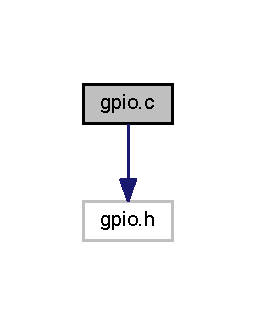
\includegraphics[width=173pt]{gpio_8c__incl}
\end{center}
\end{figure}
\subsection*{Functions}
\begin{DoxyCompactItemize}
\item 
void \mbox{\hyperlink{gpio_8c_ac724e431d2af879252de35615be2bdea}{M\+X\+\_\+\+G\+P\+I\+O\+\_\+\+Init}} (void)
\end{DoxyCompactItemize}


\subsection{Function Documentation}
\mbox{\Hypertarget{gpio_8c_ac724e431d2af879252de35615be2bdea}\label{gpio_8c_ac724e431d2af879252de35615be2bdea}} 
\index{gpio.\+c@{gpio.\+c}!M\+X\+\_\+\+G\+P\+I\+O\+\_\+\+Init@{M\+X\+\_\+\+G\+P\+I\+O\+\_\+\+Init}}
\index{M\+X\+\_\+\+G\+P\+I\+O\+\_\+\+Init@{M\+X\+\_\+\+G\+P\+I\+O\+\_\+\+Init}!gpio.\+c@{gpio.\+c}}
\subsubsection{\texorpdfstring{M\+X\+\_\+\+G\+P\+I\+O\+\_\+\+Init()}{MX\_GPIO\_Init()}}
{\footnotesize\ttfamily void M\+X\+\_\+\+G\+P\+I\+O\+\_\+\+Init (\begin{DoxyParamCaption}\item[{void}]{ }\end{DoxyParamCaption})}

File Name \+: \mbox{\hyperlink{gpio_8c}{gpio.\+c}} Description \+: This file provides code for the configuration of all used G\+P\+IO pins.

This notice applies to any and all portions of this file that are not between comment pairs U\+S\+ER C\+O\+DE B\+E\+G\+IN and U\+S\+ER C\+O\+DE E\+ND. Other portions of this file, whether inserted by the user or by software development tools are owned by their respective copyright owners.

Copyright (c) 2018 S\+T\+Microelectronics International N.\+V. All rights reserved.

Redistribution and use in source and binary forms, with or without modification, are permitted, provided that the following conditions are met\+:


\begin{DoxyEnumerate}
\item Redistribution of source code must retain the above copyright notice, this list of conditions and the following disclaimer.
\item Redistributions in binary form must reproduce the above copyright notice, this list of conditions and the following disclaimer in the documentation and/or other materials provided with the distribution.
\item Neither the name of S\+T\+Microelectronics nor the names of other contributors to this software may be used to endorse or promote products derived from this software without specific written permission.
\item This software, including modifications and/or derivative works of this software, must execute solely and exclusively on microcontroller or microprocessor devices manufactured by or for S\+T\+Microelectronics.
\item Redistribution and use of this software other than as permitted under this license is void and will automatically terminate your rights under this license.
\end{DoxyEnumerate}

T\+H\+IS S\+O\+F\+T\+W\+A\+RE IS P\+R\+O\+V\+I\+D\+ED BY S\+T\+M\+I\+C\+R\+O\+E\+L\+E\+C\+T\+R\+O\+N\+I\+CS A\+ND C\+O\+N\+T\+R\+I\+B\+U\+T\+O\+RS \char`\"{}\+A\+S I\+S\char`\"{} A\+ND A\+NY E\+X\+P\+R\+E\+SS, I\+M\+P\+L\+I\+ED OR S\+T\+A\+T\+U\+T\+O\+RY W\+A\+R\+R\+A\+N\+T\+I\+ES, I\+N\+C\+L\+U\+D\+I\+NG, B\+UT N\+OT L\+I\+M\+I\+T\+ED TO, T\+HE I\+M\+P\+L\+I\+ED W\+A\+R\+R\+A\+N\+T\+I\+ES OF M\+E\+R\+C\+H\+A\+N\+T\+A\+B\+I\+L\+I\+TY, F\+I\+T\+N\+E\+SS F\+OR A P\+A\+R\+T\+I\+C\+U\+L\+AR P\+U\+R\+P\+O\+SE A\+ND N\+O\+N-\/\+I\+N\+F\+R\+I\+N\+G\+E\+M\+E\+NT OF T\+H\+I\+RD P\+A\+R\+TY I\+N\+T\+E\+L\+L\+E\+C\+T\+U\+AL P\+R\+O\+P\+E\+R\+TY R\+I\+G\+H\+TS A\+RE D\+I\+S\+C\+L\+A\+I\+M\+ED TO T\+HE F\+U\+L\+L\+E\+ST E\+X\+T\+E\+NT P\+E\+R\+M\+I\+T\+T\+ED BY L\+AW. IN NO E\+V\+E\+NT S\+H\+A\+LL S\+T\+M\+I\+C\+R\+O\+E\+L\+E\+C\+T\+R\+O\+N\+I\+CS OR C\+O\+N\+T\+R\+I\+B\+U\+T\+O\+RS BE L\+I\+A\+B\+LE F\+OR A\+NY D\+I\+R\+E\+CT, I\+N\+D\+I\+R\+E\+CT, I\+N\+C\+I\+D\+E\+N\+T\+AL, S\+P\+E\+C\+I\+AL, E\+X\+E\+M\+P\+L\+A\+RY, OR C\+O\+N\+S\+E\+Q\+U\+E\+N\+T\+I\+AL D\+A\+M\+A\+G\+ES (I\+N\+C\+L\+U\+D\+I\+NG, B\+UT N\+OT L\+I\+M\+I\+T\+ED TO, P\+R\+O\+C\+U\+R\+E\+M\+E\+NT OF S\+U\+B\+S\+T\+I\+T\+U\+TE G\+O\+O\+DS OR S\+E\+R\+V\+I\+C\+ES; L\+O\+SS OF U\+SE, D\+A\+TA, OR P\+R\+O\+F\+I\+TS; OR B\+U\+S\+I\+N\+E\+SS I\+N\+T\+E\+R\+R\+U\+P\+T\+I\+ON) H\+O\+W\+E\+V\+ER C\+A\+U\+S\+ED A\+ND ON A\+NY T\+H\+E\+O\+RY OF L\+I\+A\+B\+I\+L\+I\+TY, W\+H\+E\+T\+H\+ER IN C\+O\+N\+T\+R\+A\+CT, S\+T\+R\+I\+CT L\+I\+A\+B\+I\+L\+I\+TY, OR T\+O\+RT (I\+N\+C\+L\+U\+D\+I\+NG N\+E\+G\+L\+I\+G\+E\+N\+CE OR O\+T\+H\+E\+R\+W\+I\+SE) A\+R\+I\+S\+I\+NG IN A\+NY W\+AY O\+UT OF T\+HE U\+SE OF T\+H\+IS S\+O\+F\+T\+W\+A\+RE, E\+V\+EN IF A\+D\+V\+I\+S\+ED OF T\+HE P\+O\+S\+S\+I\+B\+I\+L\+I\+TY OF S\+U\+CH D\+A\+M\+A\+G\+E.\+Configure pins as Analog Input Output E\+V\+E\+N\+T\+\_\+\+O\+UT E\+X\+TI 

Definition at line 70 of file gpio.\+c.

Here is the caller graph for this function\+:\nopagebreak
\begin{figure}[H]
\begin{center}
\leavevmode
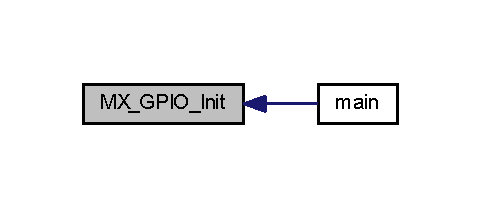
\includegraphics[width=231pt]{gpio_8c_ac724e431d2af879252de35615be2bdea_icgraph}
\end{center}
\end{figure}

\hypertarget{i2c_8c}{}\section{Src/i2c.c File Reference}
\label{i2c_8c}\index{Src/i2c.\+c@{Src/i2c.\+c}}
{\ttfamily \#include \char`\"{}i2c.\+h\char`\"{}}\newline
{\ttfamily \#include \char`\"{}gpio.\+h\char`\"{}}\newline
Include dependency graph for i2c.\+c\+:\nopagebreak
\begin{figure}[H]
\begin{center}
\leavevmode
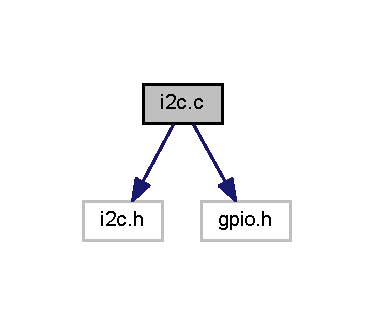
\includegraphics[width=180pt]{i2c_8c__incl}
\end{center}
\end{figure}
\subsection*{Functions}
\begin{DoxyCompactItemize}
\item 
void \mbox{\hyperlink{i2c_8c_ada6e763cfa4108a8d24cd27b75f2f489}{M\+X\+\_\+\+I2\+C1\+\_\+\+Init}} (void)
\item 
void \mbox{\hyperlink{i2c_8c_a08b1eb7b7be5b94395127e2a33b1b67e}{H\+A\+L\+\_\+\+I2\+C\+\_\+\+Msp\+Init}} (I2\+C\+\_\+\+Handle\+Type\+Def $\ast$i2c\+Handle)
\item 
void \mbox{\hyperlink{i2c_8c_adaa17249f3d5001ad363c736df31c593}{H\+A\+L\+\_\+\+I2\+C\+\_\+\+Msp\+De\+Init}} (I2\+C\+\_\+\+Handle\+Type\+Def $\ast$i2c\+Handle)
\end{DoxyCompactItemize}
\subsection*{Variables}
\begin{DoxyCompactItemize}
\item 
I2\+C\+\_\+\+Handle\+Type\+Def \mbox{\hyperlink{i2c_8c_af7b2c26e44dadaaa798a5c3d82914ba7}{hi2c1}}
\end{DoxyCompactItemize}


\subsection{Function Documentation}
\mbox{\Hypertarget{i2c_8c_adaa17249f3d5001ad363c736df31c593}\label{i2c_8c_adaa17249f3d5001ad363c736df31c593}} 
\index{i2c.\+c@{i2c.\+c}!H\+A\+L\+\_\+\+I2\+C\+\_\+\+Msp\+De\+Init@{H\+A\+L\+\_\+\+I2\+C\+\_\+\+Msp\+De\+Init}}
\index{H\+A\+L\+\_\+\+I2\+C\+\_\+\+Msp\+De\+Init@{H\+A\+L\+\_\+\+I2\+C\+\_\+\+Msp\+De\+Init}!i2c.\+c@{i2c.\+c}}
\subsubsection{\texorpdfstring{H\+A\+L\+\_\+\+I2\+C\+\_\+\+Msp\+De\+Init()}{HAL\_I2C\_MspDeInit()}}
{\footnotesize\ttfamily void H\+A\+L\+\_\+\+I2\+C\+\_\+\+Msp\+De\+Init (\begin{DoxyParamCaption}\item[{I2\+C\+\_\+\+Handle\+Type\+Def $\ast$}]{i2c\+Handle }\end{DoxyParamCaption})}

I2\+C1 G\+P\+IO Configuration ~\newline
P\+B8 -\/-\/-\/---$>$ I2\+C1\+\_\+\+S\+CL P\+B9 -\/-\/-\/---$>$ I2\+C1\+\_\+\+S\+DA

Definition at line 110 of file i2c.\+c.

\mbox{\Hypertarget{i2c_8c_a08b1eb7b7be5b94395127e2a33b1b67e}\label{i2c_8c_a08b1eb7b7be5b94395127e2a33b1b67e}} 
\index{i2c.\+c@{i2c.\+c}!H\+A\+L\+\_\+\+I2\+C\+\_\+\+Msp\+Init@{H\+A\+L\+\_\+\+I2\+C\+\_\+\+Msp\+Init}}
\index{H\+A\+L\+\_\+\+I2\+C\+\_\+\+Msp\+Init@{H\+A\+L\+\_\+\+I2\+C\+\_\+\+Msp\+Init}!i2c.\+c@{i2c.\+c}}
\subsubsection{\texorpdfstring{H\+A\+L\+\_\+\+I2\+C\+\_\+\+Msp\+Init()}{HAL\_I2C\_MspInit()}}
{\footnotesize\ttfamily void H\+A\+L\+\_\+\+I2\+C\+\_\+\+Msp\+Init (\begin{DoxyParamCaption}\item[{I2\+C\+\_\+\+Handle\+Type\+Def $\ast$}]{i2c\+Handle }\end{DoxyParamCaption})}

I2\+C1 G\+P\+IO Configuration ~\newline
P\+B8 -\/-\/-\/---$>$ I2\+C1\+\_\+\+S\+CL P\+B9 -\/-\/-\/---$>$ I2\+C1\+\_\+\+S\+DA

Definition at line 81 of file i2c.\+c.

\mbox{\Hypertarget{i2c_8c_ada6e763cfa4108a8d24cd27b75f2f489}\label{i2c_8c_ada6e763cfa4108a8d24cd27b75f2f489}} 
\index{i2c.\+c@{i2c.\+c}!M\+X\+\_\+\+I2\+C1\+\_\+\+Init@{M\+X\+\_\+\+I2\+C1\+\_\+\+Init}}
\index{M\+X\+\_\+\+I2\+C1\+\_\+\+Init@{M\+X\+\_\+\+I2\+C1\+\_\+\+Init}!i2c.\+c@{i2c.\+c}}
\subsubsection{\texorpdfstring{M\+X\+\_\+\+I2\+C1\+\_\+\+Init()}{MX\_I2C1\_Init()}}
{\footnotesize\ttfamily void M\+X\+\_\+\+I2\+C1\+\_\+\+Init (\begin{DoxyParamCaption}\item[{void}]{ }\end{DoxyParamCaption})}



Definition at line 62 of file i2c.\+c.

Here is the call graph for this function\+:\nopagebreak
\begin{figure}[H]
\begin{center}
\leavevmode
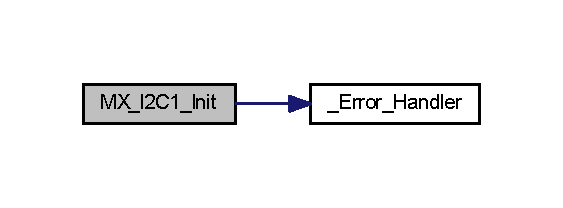
\includegraphics[width=270pt]{i2c_8c_ada6e763cfa4108a8d24cd27b75f2f489_cgraph}
\end{center}
\end{figure}
Here is the caller graph for this function\+:\nopagebreak
\begin{figure}[H]
\begin{center}
\leavevmode
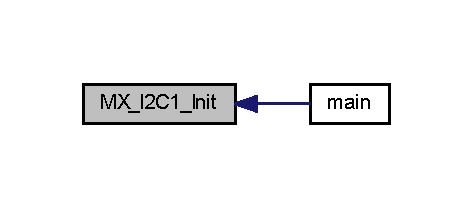
\includegraphics[width=227pt]{i2c_8c_ada6e763cfa4108a8d24cd27b75f2f489_icgraph}
\end{center}
\end{figure}


\subsection{Variable Documentation}
\mbox{\Hypertarget{i2c_8c_af7b2c26e44dadaaa798a5c3d82914ba7}\label{i2c_8c_af7b2c26e44dadaaa798a5c3d82914ba7}} 
\index{i2c.\+c@{i2c.\+c}!hi2c1@{hi2c1}}
\index{hi2c1@{hi2c1}!i2c.\+c@{i2c.\+c}}
\subsubsection{\texorpdfstring{hi2c1}{hi2c1}}
{\footnotesize\ttfamily I2\+C\+\_\+\+Handle\+Type\+Def hi2c1}

File Name \+: \mbox{\hyperlink{i2c_8c}{I2\+C.\+c}} Description \+: This file provides code for the configuration of the I2C instances.

This notice applies to any and all portions of this file that are not between comment pairs U\+S\+ER C\+O\+DE B\+E\+G\+IN and U\+S\+ER C\+O\+DE E\+ND. Other portions of this file, whether inserted by the user or by software development tools are owned by their respective copyright owners.

Copyright (c) 2018 S\+T\+Microelectronics International N.\+V. All rights reserved.

Redistribution and use in source and binary forms, with or without modification, are permitted, provided that the following conditions are met\+:


\begin{DoxyEnumerate}
\item Redistribution of source code must retain the above copyright notice, this list of conditions and the following disclaimer.
\item Redistributions in binary form must reproduce the above copyright notice, this list of conditions and the following disclaimer in the documentation and/or other materials provided with the distribution.
\item Neither the name of S\+T\+Microelectronics nor the names of other contributors to this software may be used to endorse or promote products derived from this software without specific written permission.
\item This software, including modifications and/or derivative works of this software, must execute solely and exclusively on microcontroller or microprocessor devices manufactured by or for S\+T\+Microelectronics.
\item Redistribution and use of this software other than as permitted under this license is void and will automatically terminate your rights under this license.
\end{DoxyEnumerate}

T\+H\+IS S\+O\+F\+T\+W\+A\+RE IS P\+R\+O\+V\+I\+D\+ED BY S\+T\+M\+I\+C\+R\+O\+E\+L\+E\+C\+T\+R\+O\+N\+I\+CS A\+ND C\+O\+N\+T\+R\+I\+B\+U\+T\+O\+RS \char`\"{}\+A\+S I\+S\char`\"{} A\+ND A\+NY E\+X\+P\+R\+E\+SS, I\+M\+P\+L\+I\+ED OR S\+T\+A\+T\+U\+T\+O\+RY W\+A\+R\+R\+A\+N\+T\+I\+ES, I\+N\+C\+L\+U\+D\+I\+NG, B\+UT N\+OT L\+I\+M\+I\+T\+ED TO, T\+HE I\+M\+P\+L\+I\+ED W\+A\+R\+R\+A\+N\+T\+I\+ES OF M\+E\+R\+C\+H\+A\+N\+T\+A\+B\+I\+L\+I\+TY, F\+I\+T\+N\+E\+SS F\+OR A P\+A\+R\+T\+I\+C\+U\+L\+AR P\+U\+R\+P\+O\+SE A\+ND N\+O\+N-\/\+I\+N\+F\+R\+I\+N\+G\+E\+M\+E\+NT OF T\+H\+I\+RD P\+A\+R\+TY I\+N\+T\+E\+L\+L\+E\+C\+T\+U\+AL P\+R\+O\+P\+E\+R\+TY R\+I\+G\+H\+TS A\+RE D\+I\+S\+C\+L\+A\+I\+M\+ED TO T\+HE F\+U\+L\+L\+E\+ST E\+X\+T\+E\+NT P\+E\+R\+M\+I\+T\+T\+ED BY L\+AW. IN NO E\+V\+E\+NT S\+H\+A\+LL S\+T\+M\+I\+C\+R\+O\+E\+L\+E\+C\+T\+R\+O\+N\+I\+CS OR C\+O\+N\+T\+R\+I\+B\+U\+T\+O\+RS BE L\+I\+A\+B\+LE F\+OR A\+NY D\+I\+R\+E\+CT, I\+N\+D\+I\+R\+E\+CT, I\+N\+C\+I\+D\+E\+N\+T\+AL, S\+P\+E\+C\+I\+AL, E\+X\+E\+M\+P\+L\+A\+RY, OR C\+O\+N\+S\+E\+Q\+U\+E\+N\+T\+I\+AL D\+A\+M\+A\+G\+ES (I\+N\+C\+L\+U\+D\+I\+NG, B\+UT N\+OT L\+I\+M\+I\+T\+ED TO, P\+R\+O\+C\+U\+R\+E\+M\+E\+NT OF S\+U\+B\+S\+T\+I\+T\+U\+TE G\+O\+O\+DS OR S\+E\+R\+V\+I\+C\+ES; L\+O\+SS OF U\+SE, D\+A\+TA, OR P\+R\+O\+F\+I\+TS; OR B\+U\+S\+I\+N\+E\+SS I\+N\+T\+E\+R\+R\+U\+P\+T\+I\+ON) H\+O\+W\+E\+V\+ER C\+A\+U\+S\+ED A\+ND ON A\+NY T\+H\+E\+O\+RY OF L\+I\+A\+B\+I\+L\+I\+TY, W\+H\+E\+T\+H\+ER IN C\+O\+N\+T\+R\+A\+CT, S\+T\+R\+I\+CT L\+I\+A\+B\+I\+L\+I\+TY, OR T\+O\+RT (I\+N\+C\+L\+U\+D\+I\+NG N\+E\+G\+L\+I\+G\+E\+N\+CE OR O\+T\+H\+E\+R\+W\+I\+SE) A\+R\+I\+S\+I\+NG IN A\+NY W\+AY O\+UT OF T\+HE U\+SE OF T\+H\+IS S\+O\+F\+T\+W\+A\+RE, E\+V\+EN IF A\+D\+V\+I\+S\+ED OF T\+HE P\+O\+S\+S\+I\+B\+I\+L\+I\+TY OF S\+U\+CH D\+A\+M\+A\+GE. 

Definition at line 59 of file i2c.\+c.


\hypertarget{main_8c}{}\section{Src/main.c File Reference}
\label{main_8c}\index{Src/main.\+c@{Src/main.\+c}}


\+: Main program body  


{\ttfamily \#include \char`\"{}main.\+h\char`\"{}}\newline
{\ttfamily \#include \char`\"{}stm32f4xx\+\_\+hal.\+h\char`\"{}}\newline
{\ttfamily \#include \char`\"{}spi.\+h\char`\"{}}\newline
{\ttfamily \#include \char`\"{}gpio.\+h\char`\"{}}\newline
{\ttfamily \#include \char`\"{}lcd\+\_\+driver.\+h\char`\"{}}\newline
{\ttfamily \#include $<$stdbool.\+h$>$}\newline
{\ttfamily \#include $<$stdio.\+h$>$}\newline
Include dependency graph for main.\+c\+:\nopagebreak
\begin{figure}[H]
\begin{center}
\leavevmode
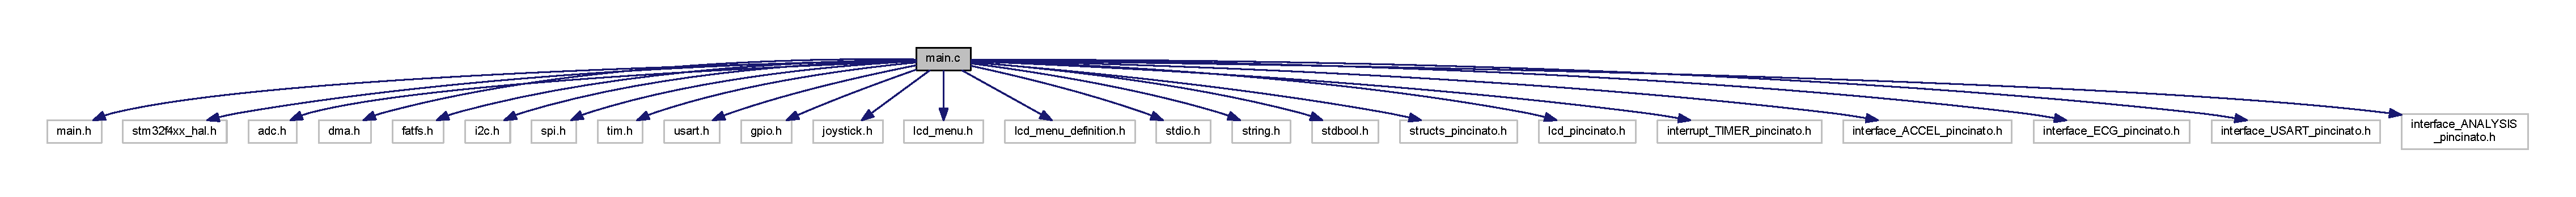
\includegraphics[width=350pt]{main_8c__incl}
\end{center}
\end{figure}
\subsection*{Functions}
\begin{DoxyCompactItemize}
\item 
void \mbox{\hyperlink{main_8c_a70af21c671abfcc773614a9a4f63d920}{System\+Clock\+\_\+\+Config}} (void)
\begin{DoxyCompactList}\small\item\em System Clock Configuration. \end{DoxyCompactList}\item 
int \mbox{\hyperlink{main_8c_a840291bc02cba5474a4cb46a9b9566fe}{main}} (void)
\begin{DoxyCompactList}\small\item\em That is Justing more un test about Doc application entry point. \end{DoxyCompactList}\item 
void \mbox{\hyperlink{main_8c_a829116a51f1db1a72ebd1120f60719d5}{\+\_\+\+Error\+\_\+\+Handler}} (char $\ast$file, int line)
\begin{DoxyCompactList}\small\item\em This function is executed in case of error occurrence. \end{DoxyCompactList}\end{DoxyCompactItemize}


\subsection{Detailed Description}
\+: Main program body 

This notice applies to any and all portions of this file that are not between comment pairs U\+S\+ER C\+O\+DE B\+E\+G\+IN and U\+S\+ER C\+O\+DE E\+ND. Other portions of this file, whether inserted by the user or by software development tools are owned by their respective copyright owners.

C\+O\+P\+Y\+R\+I\+G\+H\+T(c) 2018 S\+T\+Microelectronics

Redistribution and use in source and binary forms, with or without modification, are permitted provided that the following conditions are met\+:
\begin{DoxyEnumerate}
\item Redistributions of source code must retain the above copyright notice, this list of conditions and the following disclaimer.
\item Redistributions in binary form must reproduce the above copyright notice, this list of conditions and the following disclaimer in the documentation and/or other materials provided with the distribution.
\item Neither the name of S\+T\+Microelectronics nor the names of its contributors may be used to endorse or promote products derived from this software without specific prior written permission.
\end{DoxyEnumerate}

T\+H\+IS S\+O\+F\+T\+W\+A\+RE IS P\+R\+O\+V\+I\+D\+ED BY T\+HE C\+O\+P\+Y\+R\+I\+G\+HT H\+O\+L\+D\+E\+RS A\+ND C\+O\+N\+T\+R\+I\+B\+U\+T\+O\+RS \char`\"{}\+A\+S I\+S\char`\"{} A\+ND A\+NY E\+X\+P\+R\+E\+SS OR I\+M\+P\+L\+I\+ED W\+A\+R\+R\+A\+N\+T\+I\+ES, I\+N\+C\+L\+U\+D\+I\+NG, B\+UT N\+OT L\+I\+M\+I\+T\+ED TO, T\+HE I\+M\+P\+L\+I\+ED W\+A\+R\+R\+A\+N\+T\+I\+ES OF M\+E\+R\+C\+H\+A\+N\+T\+A\+B\+I\+L\+I\+TY A\+ND F\+I\+T\+N\+E\+SS F\+OR A P\+A\+R\+T\+I\+C\+U\+L\+AR P\+U\+R\+P\+O\+SE A\+RE D\+I\+S\+C\+L\+A\+I\+M\+ED. IN NO E\+V\+E\+NT S\+H\+A\+LL T\+HE C\+O\+P\+Y\+R\+I\+G\+HT H\+O\+L\+D\+ER OR C\+O\+N\+T\+R\+I\+B\+U\+T\+O\+RS BE L\+I\+A\+B\+LE F\+OR A\+NY D\+I\+R\+E\+CT, I\+N\+D\+I\+R\+E\+CT, I\+N\+C\+I\+D\+E\+N\+T\+AL, S\+P\+E\+C\+I\+AL, E\+X\+E\+M\+P\+L\+A\+RY, OR C\+O\+N\+S\+E\+Q\+U\+E\+N\+T\+I\+AL D\+A\+M\+A\+G\+ES (I\+N\+C\+L\+U\+D\+I\+NG, B\+UT N\+OT L\+I\+M\+I\+T\+ED TO, P\+R\+O\+C\+U\+R\+E\+M\+E\+NT OF S\+U\+B\+S\+T\+I\+T\+U\+TE G\+O\+O\+DS OR S\+E\+R\+V\+I\+C\+ES; L\+O\+SS OF U\+SE, D\+A\+TA, OR P\+R\+O\+F\+I\+TS; OR B\+U\+S\+I\+N\+E\+SS I\+N\+T\+E\+R\+R\+U\+P\+T\+I\+ON) H\+O\+W\+E\+V\+ER C\+A\+U\+S\+ED A\+ND ON A\+NY T\+H\+E\+O\+RY OF L\+I\+A\+B\+I\+L\+I\+TY, W\+H\+E\+T\+H\+ER IN C\+O\+N\+T\+R\+A\+CT, S\+T\+R\+I\+CT L\+I\+A\+B\+I\+L\+I\+TY, OR T\+O\+RT (I\+N\+C\+L\+U\+D\+I\+NG N\+E\+G\+L\+I\+G\+E\+N\+CE OR O\+T\+H\+E\+R\+W\+I\+SE) A\+R\+I\+S\+I\+NG IN A\+NY W\+AY O\+UT OF T\+HE U\+SE OF T\+H\+IS S\+O\+F\+T\+W\+A\+RE, E\+V\+EN IF A\+D\+V\+I\+S\+ED OF T\+HE P\+O\+S\+S\+I\+B\+I\+L\+I\+TY OF S\+U\+CH D\+A\+M\+A\+GE. 

\subsection{Function Documentation}
\mbox{\Hypertarget{main_8c_a829116a51f1db1a72ebd1120f60719d5}\label{main_8c_a829116a51f1db1a72ebd1120f60719d5}} 
\index{main.\+c@{main.\+c}!\+\_\+\+Error\+\_\+\+Handler@{\+\_\+\+Error\+\_\+\+Handler}}
\index{\+\_\+\+Error\+\_\+\+Handler@{\+\_\+\+Error\+\_\+\+Handler}!main.\+c@{main.\+c}}
\subsubsection{\texorpdfstring{\+\_\+\+Error\+\_\+\+Handler()}{\_Error\_Handler()}}
{\footnotesize\ttfamily void \+\_\+\+Error\+\_\+\+Handler (\begin{DoxyParamCaption}\item[{char $\ast$}]{file,  }\item[{int}]{line }\end{DoxyParamCaption})}



This function is executed in case of error occurrence. 


\begin{DoxyParams}{Parameters}
{\em file} & The file name as string. \\
\hline
{\em line} & The line in file as a number. \\
\hline
\end{DoxyParams}

\begin{DoxyRetVals}{Return values}
{\em None} & \\
\hline
\end{DoxyRetVals}


Definition at line 210 of file main.\+c.

Here is the caller graph for this function\+:
\nopagebreak
\begin{figure}[H]
\begin{center}
\leavevmode
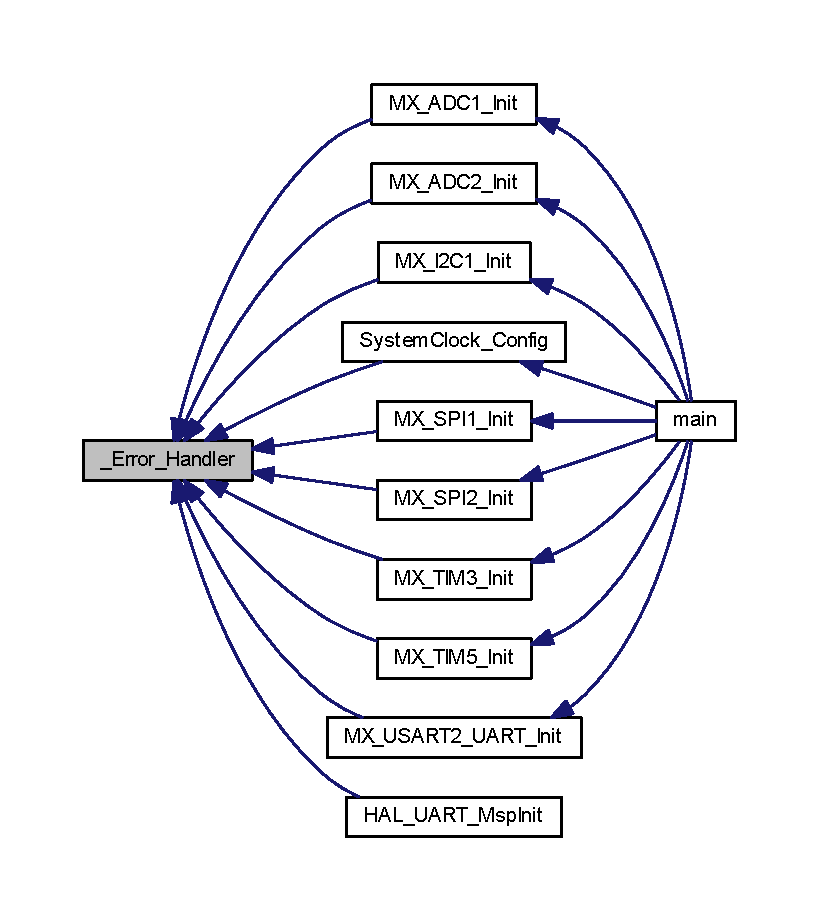
\includegraphics[width=350pt]{main_8c_a829116a51f1db1a72ebd1120f60719d5_icgraph}
\end{center}
\end{figure}
\mbox{\Hypertarget{main_8c_a840291bc02cba5474a4cb46a9b9566fe}\label{main_8c_a840291bc02cba5474a4cb46a9b9566fe}} 
\index{main.\+c@{main.\+c}!main@{main}}
\index{main@{main}!main.\+c@{main.\+c}}
\subsubsection{\texorpdfstring{main()}{main()}}
{\footnotesize\ttfamily int main (\begin{DoxyParamCaption}\item[{void}]{ }\end{DoxyParamCaption})}



That is Justing more un test about Doc application entry point. 


\begin{DoxyRetVals}{Return values}
{\em None} & \\
\hline
\end{DoxyRetVals}
\begin{DoxyWarning}{Warning}
T\+E\+ST Warning 
\end{DoxyWarning}


Definition at line 81 of file main.\+c.

Here is the call graph for this function\+:\nopagebreak
\begin{figure}[H]
\begin{center}
\leavevmode
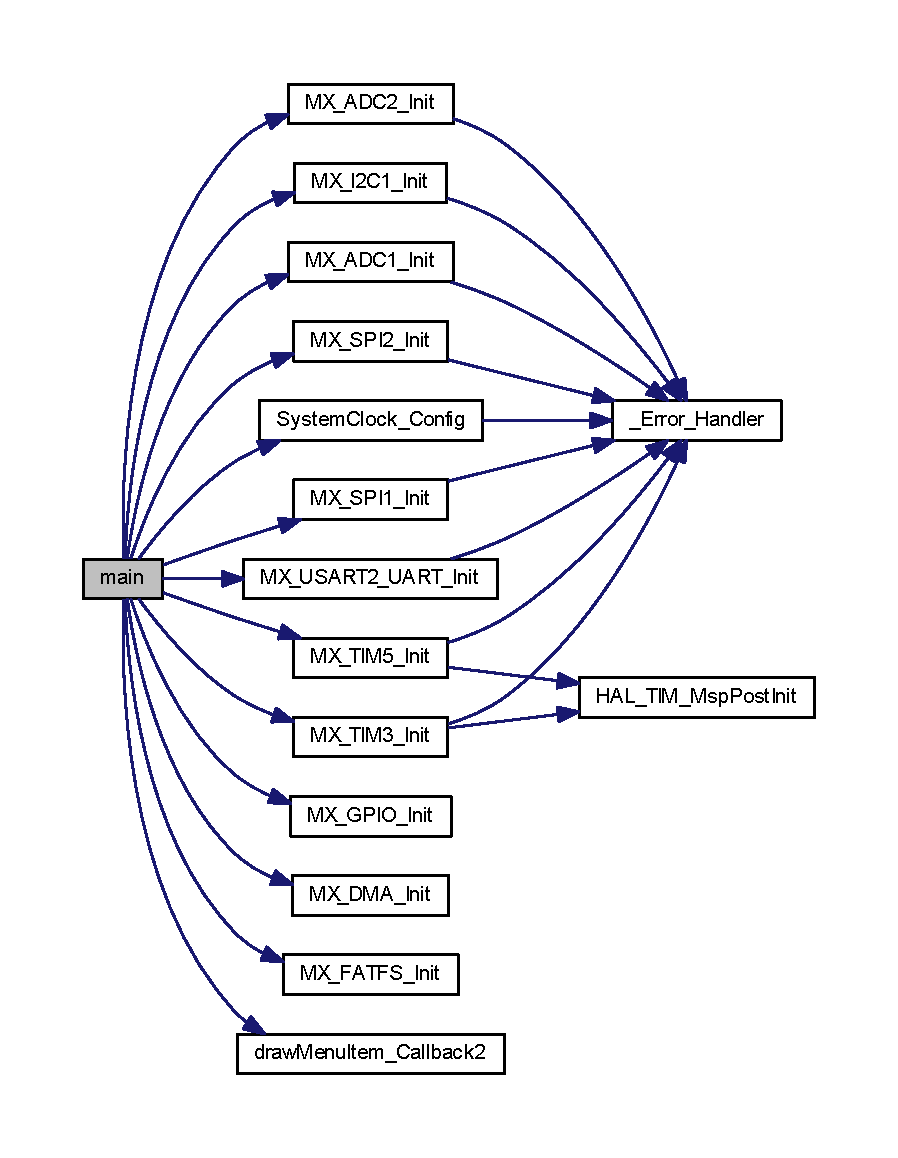
\includegraphics[width=350pt]{main_8c_a840291bc02cba5474a4cb46a9b9566fe_cgraph}
\end{center}
\end{figure}
\mbox{\Hypertarget{main_8c_a70af21c671abfcc773614a9a4f63d920}\label{main_8c_a70af21c671abfcc773614a9a4f63d920}} 
\index{main.\+c@{main.\+c}!System\+Clock\+\_\+\+Config@{System\+Clock\+\_\+\+Config}}
\index{System\+Clock\+\_\+\+Config@{System\+Clock\+\_\+\+Config}!main.\+c@{main.\+c}}
\subsubsection{\texorpdfstring{System\+Clock\+\_\+\+Config()}{SystemClock\_Config()}}
{\footnotesize\ttfamily void System\+Clock\+\_\+\+Config (\begin{DoxyParamCaption}\item[{void}]{ }\end{DoxyParamCaption})}



System Clock Configuration. 


\begin{DoxyRetVals}{Return values}
{\em None} & \\
\hline
\end{DoxyRetVals}
Configure the main internal regulator output voltage

Initializes the C\+PU, A\+HB and A\+PB busses clocks

Activate the Over-\/\+Drive mode

Initializes the C\+PU, A\+HB and A\+PB busses clocks

Configure the Systick interrupt time

Configure the Systick

Definition at line 138 of file main.\+c.

Here is the call graph for this function\+:\nopagebreak
\begin{figure}[H]
\begin{center}
\leavevmode
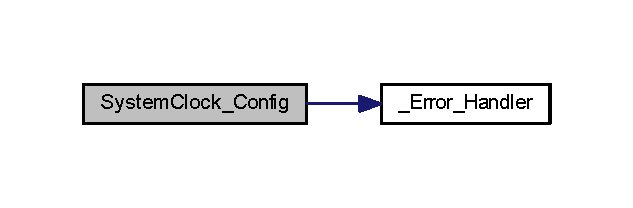
\includegraphics[width=304pt]{main_8c_a70af21c671abfcc773614a9a4f63d920_cgraph}
\end{center}
\end{figure}
Here is the caller graph for this function\+:
\nopagebreak
\begin{figure}[H]
\begin{center}
\leavevmode
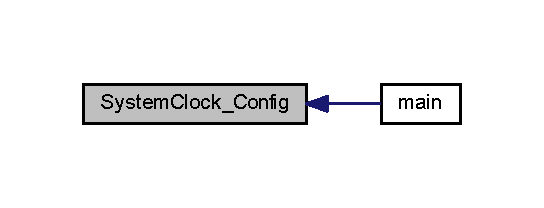
\includegraphics[width=261pt]{main_8c_a70af21c671abfcc773614a9a4f63d920_icgraph}
\end{center}
\end{figure}

\hypertarget{spi_8c}{}\section{Src/spi.c File Reference}
\label{spi_8c}\index{Src/spi.\+c@{Src/spi.\+c}}
{\ttfamily \#include \char`\"{}spi.\+h\char`\"{}}\newline
{\ttfamily \#include \char`\"{}gpio.\+h\char`\"{}}\newline
Include dependency graph for spi.\+c\+:\nopagebreak
\begin{figure}[H]
\begin{center}
\leavevmode
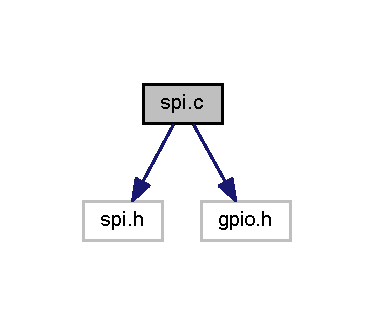
\includegraphics[width=180pt]{spi_8c__incl}
\end{center}
\end{figure}
\subsection*{Functions}
\begin{DoxyCompactItemize}
\item 
void \mbox{\hyperlink{spi_8c_af81398f9775695df0b172367651ca3e6}{M\+X\+\_\+\+S\+P\+I1\+\_\+\+Init}} (void)
\item 
void \mbox{\hyperlink{spi_8c_aea85daa666c03d85fd59edef711ebb08}{M\+X\+\_\+\+S\+P\+I2\+\_\+\+Init}} (void)
\item 
void \mbox{\hyperlink{spi_8c_a8e1dadd744299fa6f8bca0e1bcbd2c00}{H\+A\+L\+\_\+\+S\+P\+I\+\_\+\+Msp\+Init}} (S\+P\+I\+\_\+\+Handle\+Type\+Def $\ast$spi\+Handle)
\item 
void \mbox{\hyperlink{spi_8c_af9af6cae4cb9386b709196d3a3ab4f78}{H\+A\+L\+\_\+\+S\+P\+I\+\_\+\+Msp\+De\+Init}} (S\+P\+I\+\_\+\+Handle\+Type\+Def $\ast$spi\+Handle)
\end{DoxyCompactItemize}
\subsection*{Variables}
\begin{DoxyCompactItemize}
\item 
S\+P\+I\+\_\+\+Handle\+Type\+Def \mbox{\hyperlink{spi_8c_a9c6222bae4d0328dd843ae099623b40b}{hspi1}}
\item 
S\+P\+I\+\_\+\+Handle\+Type\+Def \mbox{\hyperlink{spi_8c_ab9da65f935e805137e2eb4e18c5ab224}{hspi2}}
\end{DoxyCompactItemize}


\subsection{Function Documentation}
\mbox{\Hypertarget{spi_8c_af9af6cae4cb9386b709196d3a3ab4f78}\label{spi_8c_af9af6cae4cb9386b709196d3a3ab4f78}} 
\index{spi.\+c@{spi.\+c}!H\+A\+L\+\_\+\+S\+P\+I\+\_\+\+Msp\+De\+Init@{H\+A\+L\+\_\+\+S\+P\+I\+\_\+\+Msp\+De\+Init}}
\index{H\+A\+L\+\_\+\+S\+P\+I\+\_\+\+Msp\+De\+Init@{H\+A\+L\+\_\+\+S\+P\+I\+\_\+\+Msp\+De\+Init}!spi.\+c@{spi.\+c}}
\subsubsection{\texorpdfstring{H\+A\+L\+\_\+\+S\+P\+I\+\_\+\+Msp\+De\+Init()}{HAL\_SPI\_MspDeInit()}}
{\footnotesize\ttfamily void H\+A\+L\+\_\+\+S\+P\+I\+\_\+\+Msp\+De\+Init (\begin{DoxyParamCaption}\item[{S\+P\+I\+\_\+\+Handle\+Type\+Def $\ast$}]{spi\+Handle }\end{DoxyParamCaption})}

S\+P\+I1 G\+P\+IO Configuration ~\newline
~\newline
P\+A5 ------$>$ S\+P\+I1\+\_\+\+S\+CK P\+A7 ------$>$ S\+P\+I1\+\_\+\+M\+O\+SI

S\+P\+I2 G\+P\+IO Configuration ~\newline
P\+B13 -\/-\/-\/---$>$ S\+P\+I2\+\_\+\+S\+CK P\+B14 -\/-\/-\/---$>$ S\+P\+I2\+\_\+\+M\+I\+SO P\+B15 -\/-\/-\/---$>$ S\+P\+I2\+\_\+\+M\+O\+SI

Definition at line 160 of file spi.\+c.

\mbox{\Hypertarget{spi_8c_a8e1dadd744299fa6f8bca0e1bcbd2c00}\label{spi_8c_a8e1dadd744299fa6f8bca0e1bcbd2c00}} 
\index{spi.\+c@{spi.\+c}!H\+A\+L\+\_\+\+S\+P\+I\+\_\+\+Msp\+Init@{H\+A\+L\+\_\+\+S\+P\+I\+\_\+\+Msp\+Init}}
\index{H\+A\+L\+\_\+\+S\+P\+I\+\_\+\+Msp\+Init@{H\+A\+L\+\_\+\+S\+P\+I\+\_\+\+Msp\+Init}!spi.\+c@{spi.\+c}}
\subsubsection{\texorpdfstring{H\+A\+L\+\_\+\+S\+P\+I\+\_\+\+Msp\+Init()}{HAL\_SPI\_MspInit()}}
{\footnotesize\ttfamily void H\+A\+L\+\_\+\+S\+P\+I\+\_\+\+Msp\+Init (\begin{DoxyParamCaption}\item[{S\+P\+I\+\_\+\+Handle\+Type\+Def $\ast$}]{spi\+Handle }\end{DoxyParamCaption})}

S\+P\+I1 G\+P\+IO Configuration ~\newline
~\newline
P\+A5 ------$>$ S\+P\+I1\+\_\+\+S\+CK P\+A7 ------$>$ S\+P\+I1\+\_\+\+M\+O\+SI

S\+P\+I2 G\+P\+IO Configuration ~\newline
P\+B13 -\/-\/-\/---$>$ S\+P\+I2\+\_\+\+S\+CK P\+B14 -\/-\/-\/---$>$ S\+P\+I2\+\_\+\+M\+I\+SO P\+B15 -\/-\/-\/---$>$ S\+P\+I2\+\_\+\+M\+O\+SI

Definition at line 107 of file spi.\+c.

\mbox{\Hypertarget{spi_8c_af81398f9775695df0b172367651ca3e6}\label{spi_8c_af81398f9775695df0b172367651ca3e6}} 
\index{spi.\+c@{spi.\+c}!M\+X\+\_\+\+S\+P\+I1\+\_\+\+Init@{M\+X\+\_\+\+S\+P\+I1\+\_\+\+Init}}
\index{M\+X\+\_\+\+S\+P\+I1\+\_\+\+Init@{M\+X\+\_\+\+S\+P\+I1\+\_\+\+Init}!spi.\+c@{spi.\+c}}
\subsubsection{\texorpdfstring{M\+X\+\_\+\+S\+P\+I1\+\_\+\+Init()}{MX\_SPI1\_Init()}}
{\footnotesize\ttfamily void M\+X\+\_\+\+S\+P\+I1\+\_\+\+Init (\begin{DoxyParamCaption}\item[{void}]{ }\end{DoxyParamCaption})}



Definition at line 63 of file spi.\+c.

Here is the call graph for this function\+:\nopagebreak
\begin{figure}[H]
\begin{center}
\leavevmode
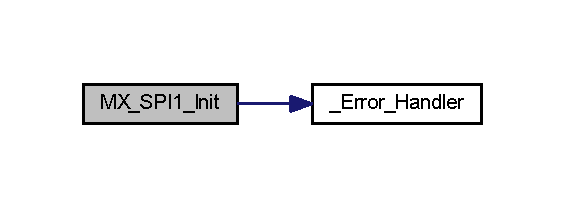
\includegraphics[width=271pt]{spi_8c_af81398f9775695df0b172367651ca3e6_cgraph}
\end{center}
\end{figure}
Here is the caller graph for this function\+:\nopagebreak
\begin{figure}[H]
\begin{center}
\leavevmode
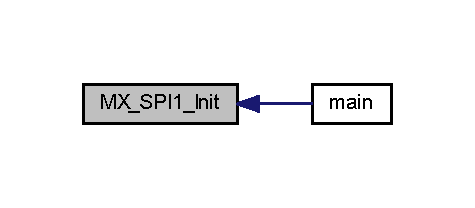
\includegraphics[width=312pt]{spi_8c_af81398f9775695df0b172367651ca3e6_icgraph}
\end{center}
\end{figure}
\mbox{\Hypertarget{spi_8c_aea85daa666c03d85fd59edef711ebb08}\label{spi_8c_aea85daa666c03d85fd59edef711ebb08}} 
\index{spi.\+c@{spi.\+c}!M\+X\+\_\+\+S\+P\+I2\+\_\+\+Init@{M\+X\+\_\+\+S\+P\+I2\+\_\+\+Init}}
\index{M\+X\+\_\+\+S\+P\+I2\+\_\+\+Init@{M\+X\+\_\+\+S\+P\+I2\+\_\+\+Init}!spi.\+c@{spi.\+c}}
\subsubsection{\texorpdfstring{M\+X\+\_\+\+S\+P\+I2\+\_\+\+Init()}{MX\_SPI2\_Init()}}
{\footnotesize\ttfamily void M\+X\+\_\+\+S\+P\+I2\+\_\+\+Init (\begin{DoxyParamCaption}\item[{void}]{ }\end{DoxyParamCaption})}



Definition at line 85 of file spi.\+c.

Here is the call graph for this function\+:\nopagebreak
\begin{figure}[H]
\begin{center}
\leavevmode
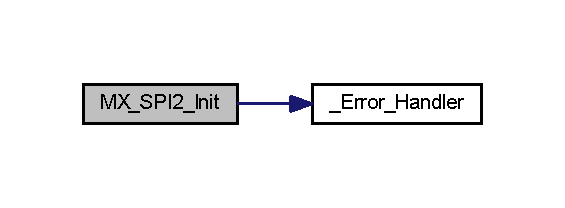
\includegraphics[width=271pt]{spi_8c_aea85daa666c03d85fd59edef711ebb08_cgraph}
\end{center}
\end{figure}
Here is the caller graph for this function\+:\nopagebreak
\begin{figure}[H]
\begin{center}
\leavevmode
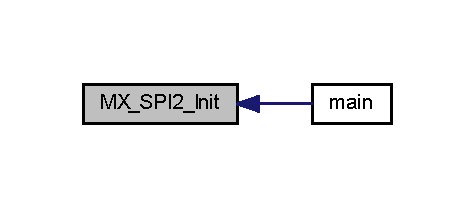
\includegraphics[width=228pt]{spi_8c_aea85daa666c03d85fd59edef711ebb08_icgraph}
\end{center}
\end{figure}


\subsection{Variable Documentation}
\mbox{\Hypertarget{spi_8c_a9c6222bae4d0328dd843ae099623b40b}\label{spi_8c_a9c6222bae4d0328dd843ae099623b40b}} 
\index{spi.\+c@{spi.\+c}!hspi1@{hspi1}}
\index{hspi1@{hspi1}!spi.\+c@{spi.\+c}}
\subsubsection{\texorpdfstring{hspi1}{hspi1}}
{\footnotesize\ttfamily S\+P\+I\+\_\+\+Handle\+Type\+Def hspi1}

File Name \+: \mbox{\hyperlink{spi_8c}{S\+P\+I.\+c}} Description \+: This file provides code for the configuration of the S\+PI instances.

This notice applies to any and all portions of this file that are not between comment pairs U\+S\+ER C\+O\+DE B\+E\+G\+IN and U\+S\+ER C\+O\+DE E\+ND. Other portions of this file, whether inserted by the user or by software development tools are owned by their respective copyright owners.

Copyright (c) 2018 S\+T\+Microelectronics International N.\+V. All rights reserved.

Redistribution and use in source and binary forms, with or without modification, are permitted, provided that the following conditions are met\+:


\begin{DoxyEnumerate}
\item Redistribution of source code must retain the above copyright notice, this list of conditions and the following disclaimer.
\item Redistributions in binary form must reproduce the above copyright notice, this list of conditions and the following disclaimer in the documentation and/or other materials provided with the distribution.
\item Neither the name of S\+T\+Microelectronics nor the names of other contributors to this software may be used to endorse or promote products derived from this software without specific written permission.
\item This software, including modifications and/or derivative works of this software, must execute solely and exclusively on microcontroller or microprocessor devices manufactured by or for S\+T\+Microelectronics.
\item Redistribution and use of this software other than as permitted under this license is void and will automatically terminate your rights under this license.
\end{DoxyEnumerate}

T\+H\+IS S\+O\+F\+T\+W\+A\+RE IS P\+R\+O\+V\+I\+D\+ED BY S\+T\+M\+I\+C\+R\+O\+E\+L\+E\+C\+T\+R\+O\+N\+I\+CS A\+ND C\+O\+N\+T\+R\+I\+B\+U\+T\+O\+RS \char`\"{}\+A\+S I\+S\char`\"{} A\+ND A\+NY E\+X\+P\+R\+E\+SS, I\+M\+P\+L\+I\+ED OR S\+T\+A\+T\+U\+T\+O\+RY W\+A\+R\+R\+A\+N\+T\+I\+ES, I\+N\+C\+L\+U\+D\+I\+NG, B\+UT N\+OT L\+I\+M\+I\+T\+ED TO, T\+HE I\+M\+P\+L\+I\+ED W\+A\+R\+R\+A\+N\+T\+I\+ES OF M\+E\+R\+C\+H\+A\+N\+T\+A\+B\+I\+L\+I\+TY, F\+I\+T\+N\+E\+SS F\+OR A P\+A\+R\+T\+I\+C\+U\+L\+AR P\+U\+R\+P\+O\+SE A\+ND N\+O\+N-\/\+I\+N\+F\+R\+I\+N\+G\+E\+M\+E\+NT OF T\+H\+I\+RD P\+A\+R\+TY I\+N\+T\+E\+L\+L\+E\+C\+T\+U\+AL P\+R\+O\+P\+E\+R\+TY R\+I\+G\+H\+TS A\+RE D\+I\+S\+C\+L\+A\+I\+M\+ED TO T\+HE F\+U\+L\+L\+E\+ST E\+X\+T\+E\+NT P\+E\+R\+M\+I\+T\+T\+ED BY L\+AW. IN NO E\+V\+E\+NT S\+H\+A\+LL S\+T\+M\+I\+C\+R\+O\+E\+L\+E\+C\+T\+R\+O\+N\+I\+CS OR C\+O\+N\+T\+R\+I\+B\+U\+T\+O\+RS BE L\+I\+A\+B\+LE F\+OR A\+NY D\+I\+R\+E\+CT, I\+N\+D\+I\+R\+E\+CT, I\+N\+C\+I\+D\+E\+N\+T\+AL, S\+P\+E\+C\+I\+AL, E\+X\+E\+M\+P\+L\+A\+RY, OR C\+O\+N\+S\+E\+Q\+U\+E\+N\+T\+I\+AL D\+A\+M\+A\+G\+ES (I\+N\+C\+L\+U\+D\+I\+NG, B\+UT N\+OT L\+I\+M\+I\+T\+ED TO, P\+R\+O\+C\+U\+R\+E\+M\+E\+NT OF S\+U\+B\+S\+T\+I\+T\+U\+TE G\+O\+O\+DS OR S\+E\+R\+V\+I\+C\+ES; L\+O\+SS OF U\+SE, D\+A\+TA, OR P\+R\+O\+F\+I\+TS; OR B\+U\+S\+I\+N\+E\+SS I\+N\+T\+E\+R\+R\+U\+P\+T\+I\+ON) H\+O\+W\+E\+V\+ER C\+A\+U\+S\+ED A\+ND ON A\+NY T\+H\+E\+O\+RY OF L\+I\+A\+B\+I\+L\+I\+TY, W\+H\+E\+T\+H\+ER IN C\+O\+N\+T\+R\+A\+CT, S\+T\+R\+I\+CT L\+I\+A\+B\+I\+L\+I\+TY, OR T\+O\+RT (I\+N\+C\+L\+U\+D\+I\+NG N\+E\+G\+L\+I\+G\+E\+N\+CE OR O\+T\+H\+E\+R\+W\+I\+SE) A\+R\+I\+S\+I\+NG IN A\+NY W\+AY O\+UT OF T\+HE U\+SE OF T\+H\+IS S\+O\+F\+T\+W\+A\+RE, E\+V\+EN IF A\+D\+V\+I\+S\+ED OF T\+HE P\+O\+S\+S\+I\+B\+I\+L\+I\+TY OF S\+U\+CH D\+A\+M\+A\+GE. 

Definition at line 59 of file spi.\+c.

\mbox{\Hypertarget{spi_8c_ab9da65f935e805137e2eb4e18c5ab224}\label{spi_8c_ab9da65f935e805137e2eb4e18c5ab224}} 
\index{spi.\+c@{spi.\+c}!hspi2@{hspi2}}
\index{hspi2@{hspi2}!spi.\+c@{spi.\+c}}
\subsubsection{\texorpdfstring{hspi2}{hspi2}}
{\footnotesize\ttfamily S\+P\+I\+\_\+\+Handle\+Type\+Def hspi2}



Definition at line 60 of file spi.\+c.


\hypertarget{stm32f4xx__hal__msp_8c}{}\section{stm32f4xx\+\_\+hal\+\_\+msp.\+c File Reference}
\label{stm32f4xx__hal__msp_8c}\index{stm32f4xx\+\_\+hal\+\_\+msp.\+c@{stm32f4xx\+\_\+hal\+\_\+msp.\+c}}
{\ttfamily \#include \char`\"{}stm32f4xx\+\_\+hal.\+h\char`\"{}}\newline
Include dependency graph for stm32f4xx\+\_\+hal\+\_\+msp.\+c\+:
\nopagebreak
\begin{figure}[H]
\begin{center}
\leavevmode
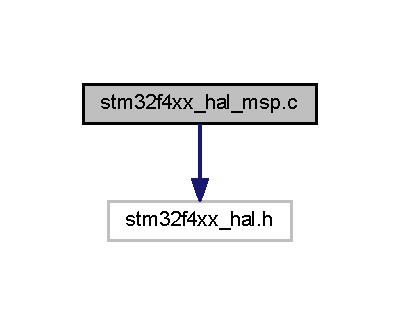
\includegraphics[width=192pt]{stm32f4xx__hal__msp_8c__incl}
\end{center}
\end{figure}
\subsection*{Functions}
\begin{DoxyCompactItemize}
\item 
void \mbox{\hyperlink{stm32f4xx__hal__msp_8c_a47642651029b93e3f9c9edad46bd27b4}{\+\_\+\+Error\+\_\+\+Handler}} (char $\ast$, int)
\begin{DoxyCompactList}\small\item\em This function is executed in case of error occurrence. \end{DoxyCompactList}\item 
void \mbox{\hyperlink{stm32f4xx__hal__msp_8c_ae4fb8e66865c87d0ebab74a726a6891f}{H\+A\+L\+\_\+\+Msp\+Init}} (void)
\end{DoxyCompactItemize}


\subsection{Function Documentation}
\mbox{\Hypertarget{stm32f4xx__hal__msp_8c_a47642651029b93e3f9c9edad46bd27b4}\label{stm32f4xx__hal__msp_8c_a47642651029b93e3f9c9edad46bd27b4}} 
\index{stm32f4xx\+\_\+hal\+\_\+msp.\+c@{stm32f4xx\+\_\+hal\+\_\+msp.\+c}!\+\_\+\+Error\+\_\+\+Handler@{\+\_\+\+Error\+\_\+\+Handler}}
\index{\+\_\+\+Error\+\_\+\+Handler@{\+\_\+\+Error\+\_\+\+Handler}!stm32f4xx\+\_\+hal\+\_\+msp.\+c@{stm32f4xx\+\_\+hal\+\_\+msp.\+c}}
\subsubsection{\texorpdfstring{\+\_\+\+Error\+\_\+\+Handler()}{\_Error\_Handler()}}
{\footnotesize\ttfamily void \+\_\+\+Error\+\_\+\+Handler (\begin{DoxyParamCaption}\item[{char $\ast$}]{file,  }\item[{int}]{line }\end{DoxyParamCaption})}



This function is executed in case of error occurrence. 

File Name \+: \mbox{\hyperlink{stm32f4xx__hal__msp_8c}{stm32f4xx\+\_\+hal\+\_\+msp.\+c}} Description \+: This file provides code for the M\+SP Initialization and de-\/\+Initialization codes.

This notice applies to any and all portions of this file that are not between comment pairs U\+S\+ER C\+O\+DE B\+E\+G\+IN and U\+S\+ER C\+O\+DE E\+ND. Other portions of this file, whether inserted by the user or by software development tools are owned by their respective copyright owners.

Copyright (c) 2018 S\+T\+Microelectronics International N.\+V. All rights reserved.

Redistribution and use in source and binary forms, with or without modification, are permitted, provided that the following conditions are met\+:


\begin{DoxyEnumerate}
\item Redistribution of source code must retain the above copyright notice, this list of conditions and the following disclaimer.
\item Redistributions in binary form must reproduce the above copyright notice, this list of conditions and the following disclaimer in the documentation and/or other materials provided with the distribution.
\item Neither the name of S\+T\+Microelectronics nor the names of other contributors to this software may be used to endorse or promote products derived from this software without specific written permission.
\item This software, including modifications and/or derivative works of this software, must execute solely and exclusively on microcontroller or microprocessor devices manufactured by or for S\+T\+Microelectronics.
\item Redistribution and use of this software other than as permitted under this license is void and will automatically terminate your rights under this license.
\end{DoxyEnumerate}

T\+H\+IS S\+O\+F\+T\+W\+A\+RE IS P\+R\+O\+V\+I\+D\+ED BY S\+T\+M\+I\+C\+R\+O\+E\+L\+E\+C\+T\+R\+O\+N\+I\+CS A\+ND C\+O\+N\+T\+R\+I\+B\+U\+T\+O\+RS \char`\"{}\+A\+S I\+S\char`\"{} A\+ND A\+NY E\+X\+P\+R\+E\+SS, I\+M\+P\+L\+I\+ED OR S\+T\+A\+T\+U\+T\+O\+RY W\+A\+R\+R\+A\+N\+T\+I\+ES, I\+N\+C\+L\+U\+D\+I\+NG, B\+UT N\+OT L\+I\+M\+I\+T\+ED TO, T\+HE I\+M\+P\+L\+I\+ED W\+A\+R\+R\+A\+N\+T\+I\+ES OF M\+E\+R\+C\+H\+A\+N\+T\+A\+B\+I\+L\+I\+TY, F\+I\+T\+N\+E\+SS F\+OR A P\+A\+R\+T\+I\+C\+U\+L\+AR P\+U\+R\+P\+O\+SE A\+ND N\+O\+N-\/\+I\+N\+F\+R\+I\+N\+G\+E\+M\+E\+NT OF T\+H\+I\+RD P\+A\+R\+TY I\+N\+T\+E\+L\+L\+E\+C\+T\+U\+AL P\+R\+O\+P\+E\+R\+TY R\+I\+G\+H\+TS A\+RE D\+I\+S\+C\+L\+A\+I\+M\+ED TO T\+HE F\+U\+L\+L\+E\+ST E\+X\+T\+E\+NT P\+E\+R\+M\+I\+T\+T\+ED BY L\+AW. IN NO E\+V\+E\+NT S\+H\+A\+LL S\+T\+M\+I\+C\+R\+O\+E\+L\+E\+C\+T\+R\+O\+N\+I\+CS OR C\+O\+N\+T\+R\+I\+B\+U\+T\+O\+RS BE L\+I\+A\+B\+LE F\+OR A\+NY D\+I\+R\+E\+CT, I\+N\+D\+I\+R\+E\+CT, I\+N\+C\+I\+D\+E\+N\+T\+AL, S\+P\+E\+C\+I\+AL, E\+X\+E\+M\+P\+L\+A\+RY, OR C\+O\+N\+S\+E\+Q\+U\+E\+N\+T\+I\+AL D\+A\+M\+A\+G\+ES (I\+N\+C\+L\+U\+D\+I\+NG, B\+UT N\+OT L\+I\+M\+I\+T\+ED TO, P\+R\+O\+C\+U\+R\+E\+M\+E\+NT OF S\+U\+B\+S\+T\+I\+T\+U\+TE G\+O\+O\+DS OR S\+E\+R\+V\+I\+C\+ES; L\+O\+SS OF U\+SE, D\+A\+TA, OR P\+R\+O\+F\+I\+TS; OR B\+U\+S\+I\+N\+E\+SS I\+N\+T\+E\+R\+R\+U\+P\+T\+I\+ON) H\+O\+W\+E\+V\+ER C\+A\+U\+S\+ED A\+ND ON A\+NY T\+H\+E\+O\+RY OF L\+I\+A\+B\+I\+L\+I\+TY, W\+H\+E\+T\+H\+ER IN C\+O\+N\+T\+R\+A\+CT, S\+T\+R\+I\+CT L\+I\+A\+B\+I\+L\+I\+TY, OR T\+O\+RT (I\+N\+C\+L\+U\+D\+I\+NG N\+E\+G\+L\+I\+G\+E\+N\+CE OR O\+T\+H\+E\+R\+W\+I\+SE) A\+R\+I\+S\+I\+NG IN A\+NY W\+AY O\+UT OF T\+HE U\+SE OF T\+H\+IS S\+O\+F\+T\+W\+A\+RE, E\+V\+EN IF A\+D\+V\+I\+S\+ED OF T\+HE P\+O\+S\+S\+I\+B\+I\+L\+I\+TY OF S\+U\+CH D\+A\+M\+A\+GE.


\begin{DoxyParams}{Parameters}
{\em file} & The file name as string. \\
\hline
{\em line} & The line in file as a number. \\
\hline
\end{DoxyParams}

\begin{DoxyRetVals}{Return values}
{\em None} & \\
\hline
\end{DoxyRetVals}


Definition at line 437 of file main.\+c.

Here is the caller graph for this function\+:
\nopagebreak
\begin{figure}[H]
\begin{center}
\leavevmode
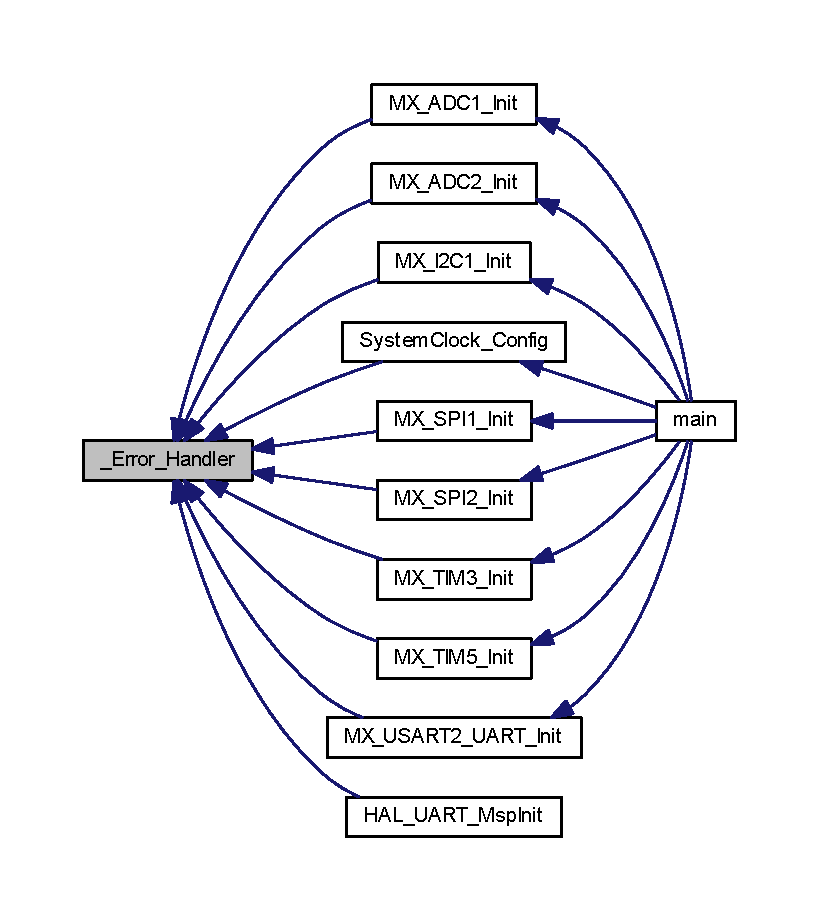
\includegraphics[width=350pt]{stm32f4xx__hal__msp_8c_a47642651029b93e3f9c9edad46bd27b4_icgraph}
\end{center}
\end{figure}
\mbox{\Hypertarget{stm32f4xx__hal__msp_8c_ae4fb8e66865c87d0ebab74a726a6891f}\label{stm32f4xx__hal__msp_8c_ae4fb8e66865c87d0ebab74a726a6891f}} 
\index{stm32f4xx\+\_\+hal\+\_\+msp.\+c@{stm32f4xx\+\_\+hal\+\_\+msp.\+c}!H\+A\+L\+\_\+\+Msp\+Init@{H\+A\+L\+\_\+\+Msp\+Init}}
\index{H\+A\+L\+\_\+\+Msp\+Init@{H\+A\+L\+\_\+\+Msp\+Init}!stm32f4xx\+\_\+hal\+\_\+msp.\+c@{stm32f4xx\+\_\+hal\+\_\+msp.\+c}}
\subsubsection{\texorpdfstring{H\+A\+L\+\_\+\+Msp\+Init()}{HAL\_MspInit()}}
{\footnotesize\ttfamily void H\+A\+L\+\_\+\+Msp\+Init (\begin{DoxyParamCaption}\item[{void}]{ }\end{DoxyParamCaption})}

Initializes the Global M\+SP. 

Definition at line 58 of file stm32f4xx\+\_\+hal\+\_\+msp.\+c.


\hypertarget{stm32f4xx__it_8c}{}\section{stm32f4xx\+\_\+it.\+c File Reference}
\label{stm32f4xx__it_8c}\index{stm32f4xx\+\_\+it.\+c@{stm32f4xx\+\_\+it.\+c}}


Interrupt Service Routines.  


{\ttfamily \#include \char`\"{}stm32f4xx\+\_\+hal.\+h\char`\"{}}\newline
{\ttfamily \#include \char`\"{}stm32f4xx.\+h\char`\"{}}\newline
{\ttfamily \#include \char`\"{}stm32f4xx\+\_\+it.\+h\char`\"{}}\newline
Include dependency graph for stm32f4xx\+\_\+it.\+c\+:
\nopagebreak
\begin{figure}[H]
\begin{center}
\leavevmode
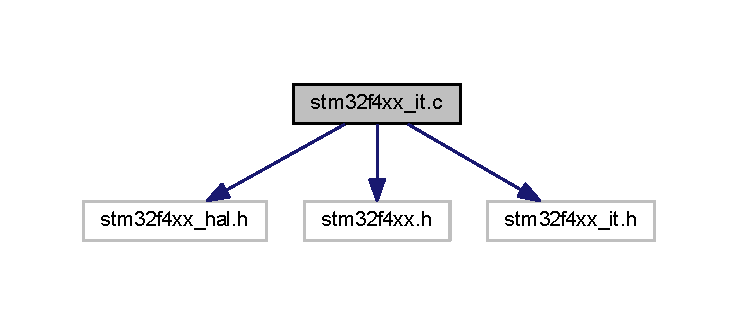
\includegraphics[width=350pt]{stm32f4xx__it_8c__incl}
\end{center}
\end{figure}
\subsection*{Functions}
\begin{DoxyCompactItemize}
\item 
void \mbox{\hyperlink{stm32f4xx__it_8c_a6ad7a5e3ee69cb6db6a6b9111ba898bc}{N\+M\+I\+\_\+\+Handler}} (void)
\begin{DoxyCompactList}\small\item\em This function handles Non maskable interrupt. \end{DoxyCompactList}\item 
void \mbox{\hyperlink{stm32f4xx__it_8c_a2bffc10d5bd4106753b7c30e86903bea}{Hard\+Fault\+\_\+\+Handler}} (void)
\begin{DoxyCompactList}\small\item\em This function handles Hard fault interrupt. \end{DoxyCompactList}\item 
void \mbox{\hyperlink{stm32f4xx__it_8c_a3150f74512510287a942624aa9b44cc5}{Mem\+Manage\+\_\+\+Handler}} (void)
\begin{DoxyCompactList}\small\item\em This function handles Memory management fault. \end{DoxyCompactList}\item 
void \mbox{\hyperlink{stm32f4xx__it_8c_a850cefb17a977292ae5eb4cafa9976c3}{Bus\+Fault\+\_\+\+Handler}} (void)
\begin{DoxyCompactList}\small\item\em This function handles Pre-\/fetch fault, memory access fault. \end{DoxyCompactList}\item 
void \mbox{\hyperlink{stm32f4xx__it_8c_a1d98923de2ed6b7309b66f9ba2971647}{Usage\+Fault\+\_\+\+Handler}} (void)
\begin{DoxyCompactList}\small\item\em This function handles Undefined instruction or illegal state. \end{DoxyCompactList}\item 
void \mbox{\hyperlink{stm32f4xx__it_8c_a3e5ddb3df0d62f2dc357e64a3f04a6ce}{S\+V\+C\+\_\+\+Handler}} (void)
\begin{DoxyCompactList}\small\item\em This function handles System service call via S\+WI instruction. \end{DoxyCompactList}\item 
void \mbox{\hyperlink{stm32f4xx__it_8c_adbdfb05858cc36fc520974df37ec3cb0}{Debug\+Mon\+\_\+\+Handler}} (void)
\begin{DoxyCompactList}\small\item\em This function handles Debug monitor. \end{DoxyCompactList}\item 
void \mbox{\hyperlink{stm32f4xx__it_8c_a6303e1f258cbdc1f970ce579cc015623}{Pend\+S\+V\+\_\+\+Handler}} (void)
\begin{DoxyCompactList}\small\item\em This function handles Pendable request for system service. \end{DoxyCompactList}\item 
void \mbox{\hyperlink{stm32f4xx__it_8c_ab5e09814056d617c521549e542639b7e}{Sys\+Tick\+\_\+\+Handler}} (void)
\begin{DoxyCompactList}\small\item\em This function handles System tick timer. \end{DoxyCompactList}\item 
void \mbox{\hyperlink{stm32f4xx__it_8c_ac201b60d58b0eba2ce0b55710eb3c4d0}{D\+M\+A1\+\_\+\+Stream5\+\_\+\+I\+R\+Q\+Handler}} (void)
\begin{DoxyCompactList}\small\item\em This function handles D\+M\+A1 stream5 global interrupt. \end{DoxyCompactList}\item 
void \mbox{\hyperlink{stm32f4xx__it_8c_aa28fd448462a6347589129f63bb0a388}{D\+M\+A1\+\_\+\+Stream6\+\_\+\+I\+R\+Q\+Handler}} (void)
\begin{DoxyCompactList}\small\item\em This function handles D\+M\+A1 stream6 global interrupt. \end{DoxyCompactList}\item 
void \mbox{\hyperlink{stm32f4xx__it_8c_a06406eadf297fa89a6eaf9586b227a69}{A\+D\+C\+\_\+\+I\+R\+Q\+Handler}} (void)
\begin{DoxyCompactList}\small\item\em This function handles A\+D\+C1, A\+D\+C2 and A\+D\+C3 interrupts. \end{DoxyCompactList}\item 
void \mbox{\hyperlink{stm32f4xx__it_8c_ac8e51d2183b5230cbd5481f8867adce9}{T\+I\+M3\+\_\+\+I\+R\+Q\+Handler}} (void)
\begin{DoxyCompactList}\small\item\em This function handles T\+I\+M3 global interrupt. \end{DoxyCompactList}\item 
void \mbox{\hyperlink{stm32f4xx__it_8c_a0ca6fd0e6f77921dd1123539857ba0a8}{U\+S\+A\+R\+T2\+\_\+\+I\+R\+Q\+Handler}} (void)
\begin{DoxyCompactList}\small\item\em This function handles U\+S\+A\+R\+T2 global interrupt. \end{DoxyCompactList}\item 
void \mbox{\hyperlink{stm32f4xx__it_8c_a5e66446caf21dd90191dc07a13ce2378}{T\+I\+M5\+\_\+\+I\+R\+Q\+Handler}} (void)
\begin{DoxyCompactList}\small\item\em This function handles T\+I\+M5 global interrupt. \end{DoxyCompactList}\end{DoxyCompactItemize}
\subsection*{Variables}
\begin{DoxyCompactItemize}
\item 
A\+D\+C\+\_\+\+Handle\+Type\+Def \mbox{\hyperlink{stm32f4xx__it_8c_a22b804736f5648d52f639b2647d4ed13}{hadc1}}
\item 
A\+D\+C\+\_\+\+Handle\+Type\+Def \mbox{\hyperlink{stm32f4xx__it_8c_acd9221f1aa19aebfe0b744947f2daf49}{hadc2}}
\item 
T\+I\+M\+\_\+\+Handle\+Type\+Def \mbox{\hyperlink{stm32f4xx__it_8c_aac3d2c59ee0e3bbae1b99529a154eb62}{htim3}}
\item 
T\+I\+M\+\_\+\+Handle\+Type\+Def \mbox{\hyperlink{stm32f4xx__it_8c_acefaeaaa3856ddddae7083b2d220fe4b}{htim5}}
\item 
D\+M\+A\+\_\+\+Handle\+Type\+Def \mbox{\hyperlink{stm32f4xx__it_8c_a0083b476c2a75ab9fb2ccbed0048857e}{hdma\+\_\+usart2\+\_\+tx}}
\item 
D\+M\+A\+\_\+\+Handle\+Type\+Def \mbox{\hyperlink{stm32f4xx__it_8c_a784aa25dc7e4580cfbf80658340f482c}{hdma\+\_\+usart2\+\_\+rx}}
\item 
U\+A\+R\+T\+\_\+\+Handle\+Type\+Def \mbox{\hyperlink{stm32f4xx__it_8c_aa9479c261d65eecedd3d9582f7f0f89c}{huart2}}
\end{DoxyCompactItemize}


\subsection{Detailed Description}
Interrupt Service Routines. 

C\+O\+P\+Y\+R\+I\+G\+H\+T(c) 2018 S\+T\+Microelectronics

Redistribution and use in source and binary forms, with or without modification, are permitted provided that the following conditions are met\+:
\begin{DoxyEnumerate}
\item Redistributions of source code must retain the above copyright notice, this list of conditions and the following disclaimer.
\item Redistributions in binary form must reproduce the above copyright notice, this list of conditions and the following disclaimer in the documentation and/or other materials provided with the distribution.
\item Neither the name of S\+T\+Microelectronics nor the names of its contributors may be used to endorse or promote products derived from this software without specific prior written permission.
\end{DoxyEnumerate}

T\+H\+IS S\+O\+F\+T\+W\+A\+RE IS P\+R\+O\+V\+I\+D\+ED BY T\+HE C\+O\+P\+Y\+R\+I\+G\+HT H\+O\+L\+D\+E\+RS A\+ND C\+O\+N\+T\+R\+I\+B\+U\+T\+O\+RS \char`\"{}\+A\+S I\+S\char`\"{} A\+ND A\+NY E\+X\+P\+R\+E\+SS OR I\+M\+P\+L\+I\+ED W\+A\+R\+R\+A\+N\+T\+I\+ES, I\+N\+C\+L\+U\+D\+I\+NG, B\+UT N\+OT L\+I\+M\+I\+T\+ED TO, T\+HE I\+M\+P\+L\+I\+ED W\+A\+R\+R\+A\+N\+T\+I\+ES OF M\+E\+R\+C\+H\+A\+N\+T\+A\+B\+I\+L\+I\+TY A\+ND F\+I\+T\+N\+E\+SS F\+OR A P\+A\+R\+T\+I\+C\+U\+L\+AR P\+U\+R\+P\+O\+SE A\+RE D\+I\+S\+C\+L\+A\+I\+M\+ED. IN NO E\+V\+E\+NT S\+H\+A\+LL T\+HE C\+O\+P\+Y\+R\+I\+G\+HT H\+O\+L\+D\+ER OR C\+O\+N\+T\+R\+I\+B\+U\+T\+O\+RS BE L\+I\+A\+B\+LE F\+OR A\+NY D\+I\+R\+E\+CT, I\+N\+D\+I\+R\+E\+CT, I\+N\+C\+I\+D\+E\+N\+T\+AL, S\+P\+E\+C\+I\+AL, E\+X\+E\+M\+P\+L\+A\+RY, OR C\+O\+N\+S\+E\+Q\+U\+E\+N\+T\+I\+AL D\+A\+M\+A\+G\+ES (I\+N\+C\+L\+U\+D\+I\+NG, B\+UT N\+OT L\+I\+M\+I\+T\+ED TO, P\+R\+O\+C\+U\+R\+E\+M\+E\+NT OF S\+U\+B\+S\+T\+I\+T\+U\+TE G\+O\+O\+DS OR S\+E\+R\+V\+I\+C\+ES; L\+O\+SS OF U\+SE, D\+A\+TA, OR P\+R\+O\+F\+I\+TS; OR B\+U\+S\+I\+N\+E\+SS I\+N\+T\+E\+R\+R\+U\+P\+T\+I\+ON) H\+O\+W\+E\+V\+ER C\+A\+U\+S\+ED A\+ND ON A\+NY T\+H\+E\+O\+RY OF L\+I\+A\+B\+I\+L\+I\+TY, W\+H\+E\+T\+H\+ER IN C\+O\+N\+T\+R\+A\+CT, S\+T\+R\+I\+CT L\+I\+A\+B\+I\+L\+I\+TY, OR T\+O\+RT (I\+N\+C\+L\+U\+D\+I\+NG N\+E\+G\+L\+I\+G\+E\+N\+CE OR O\+T\+H\+E\+R\+W\+I\+SE) A\+R\+I\+S\+I\+NG IN A\+NY W\+AY O\+UT OF T\+HE U\+SE OF T\+H\+IS S\+O\+F\+T\+W\+A\+RE, E\+V\+EN IF A\+D\+V\+I\+S\+ED OF T\+HE P\+O\+S\+S\+I\+B\+I\+L\+I\+TY OF S\+U\+CH D\+A\+M\+A\+GE. 

\subsection{Function Documentation}
\mbox{\Hypertarget{stm32f4xx__it_8c_a06406eadf297fa89a6eaf9586b227a69}\label{stm32f4xx__it_8c_a06406eadf297fa89a6eaf9586b227a69}} 
\index{stm32f4xx\+\_\+it.\+c@{stm32f4xx\+\_\+it.\+c}!A\+D\+C\+\_\+\+I\+R\+Q\+Handler@{A\+D\+C\+\_\+\+I\+R\+Q\+Handler}}
\index{A\+D\+C\+\_\+\+I\+R\+Q\+Handler@{A\+D\+C\+\_\+\+I\+R\+Q\+Handler}!stm32f4xx\+\_\+it.\+c@{stm32f4xx\+\_\+it.\+c}}
\subsubsection{\texorpdfstring{A\+D\+C\+\_\+\+I\+R\+Q\+Handler()}{ADC\_IRQHandler()}}
{\footnotesize\ttfamily void A\+D\+C\+\_\+\+I\+R\+Q\+Handler (\begin{DoxyParamCaption}\item[{void}]{ }\end{DoxyParamCaption})}



This function handles A\+D\+C1, A\+D\+C2 and A\+D\+C3 interrupts. 



Definition at line 232 of file stm32f4xx\+\_\+it.\+c.

\mbox{\Hypertarget{stm32f4xx__it_8c_a850cefb17a977292ae5eb4cafa9976c3}\label{stm32f4xx__it_8c_a850cefb17a977292ae5eb4cafa9976c3}} 
\index{stm32f4xx\+\_\+it.\+c@{stm32f4xx\+\_\+it.\+c}!Bus\+Fault\+\_\+\+Handler@{Bus\+Fault\+\_\+\+Handler}}
\index{Bus\+Fault\+\_\+\+Handler@{Bus\+Fault\+\_\+\+Handler}!stm32f4xx\+\_\+it.\+c@{stm32f4xx\+\_\+it.\+c}}
\subsubsection{\texorpdfstring{Bus\+Fault\+\_\+\+Handler()}{BusFault\_Handler()}}
{\footnotesize\ttfamily void Bus\+Fault\+\_\+\+Handler (\begin{DoxyParamCaption}\item[{void}]{ }\end{DoxyParamCaption})}



This function handles Pre-\/fetch fault, memory access fault. 



Definition at line 107 of file stm32f4xx\+\_\+it.\+c.

\mbox{\Hypertarget{stm32f4xx__it_8c_adbdfb05858cc36fc520974df37ec3cb0}\label{stm32f4xx__it_8c_adbdfb05858cc36fc520974df37ec3cb0}} 
\index{stm32f4xx\+\_\+it.\+c@{stm32f4xx\+\_\+it.\+c}!Debug\+Mon\+\_\+\+Handler@{Debug\+Mon\+\_\+\+Handler}}
\index{Debug\+Mon\+\_\+\+Handler@{Debug\+Mon\+\_\+\+Handler}!stm32f4xx\+\_\+it.\+c@{stm32f4xx\+\_\+it.\+c}}
\subsubsection{\texorpdfstring{Debug\+Mon\+\_\+\+Handler()}{DebugMon\_Handler()}}
{\footnotesize\ttfamily void Debug\+Mon\+\_\+\+Handler (\begin{DoxyParamCaption}\item[{void}]{ }\end{DoxyParamCaption})}



This function handles Debug monitor. 



Definition at line 156 of file stm32f4xx\+\_\+it.\+c.

\mbox{\Hypertarget{stm32f4xx__it_8c_ac201b60d58b0eba2ce0b55710eb3c4d0}\label{stm32f4xx__it_8c_ac201b60d58b0eba2ce0b55710eb3c4d0}} 
\index{stm32f4xx\+\_\+it.\+c@{stm32f4xx\+\_\+it.\+c}!D\+M\+A1\+\_\+\+Stream5\+\_\+\+I\+R\+Q\+Handler@{D\+M\+A1\+\_\+\+Stream5\+\_\+\+I\+R\+Q\+Handler}}
\index{D\+M\+A1\+\_\+\+Stream5\+\_\+\+I\+R\+Q\+Handler@{D\+M\+A1\+\_\+\+Stream5\+\_\+\+I\+R\+Q\+Handler}!stm32f4xx\+\_\+it.\+c@{stm32f4xx\+\_\+it.\+c}}
\subsubsection{\texorpdfstring{D\+M\+A1\+\_\+\+Stream5\+\_\+\+I\+R\+Q\+Handler()}{DMA1\_Stream5\_IRQHandler()}}
{\footnotesize\ttfamily void D\+M\+A1\+\_\+\+Stream5\+\_\+\+I\+R\+Q\+Handler (\begin{DoxyParamCaption}\item[{void}]{ }\end{DoxyParamCaption})}



This function handles D\+M\+A1 stream5 global interrupt. 



Definition at line 204 of file stm32f4xx\+\_\+it.\+c.

\mbox{\Hypertarget{stm32f4xx__it_8c_aa28fd448462a6347589129f63bb0a388}\label{stm32f4xx__it_8c_aa28fd448462a6347589129f63bb0a388}} 
\index{stm32f4xx\+\_\+it.\+c@{stm32f4xx\+\_\+it.\+c}!D\+M\+A1\+\_\+\+Stream6\+\_\+\+I\+R\+Q\+Handler@{D\+M\+A1\+\_\+\+Stream6\+\_\+\+I\+R\+Q\+Handler}}
\index{D\+M\+A1\+\_\+\+Stream6\+\_\+\+I\+R\+Q\+Handler@{D\+M\+A1\+\_\+\+Stream6\+\_\+\+I\+R\+Q\+Handler}!stm32f4xx\+\_\+it.\+c@{stm32f4xx\+\_\+it.\+c}}
\subsubsection{\texorpdfstring{D\+M\+A1\+\_\+\+Stream6\+\_\+\+I\+R\+Q\+Handler()}{DMA1\_Stream6\_IRQHandler()}}
{\footnotesize\ttfamily void D\+M\+A1\+\_\+\+Stream6\+\_\+\+I\+R\+Q\+Handler (\begin{DoxyParamCaption}\item[{void}]{ }\end{DoxyParamCaption})}



This function handles D\+M\+A1 stream6 global interrupt. 



Definition at line 218 of file stm32f4xx\+\_\+it.\+c.

\mbox{\Hypertarget{stm32f4xx__it_8c_a2bffc10d5bd4106753b7c30e86903bea}\label{stm32f4xx__it_8c_a2bffc10d5bd4106753b7c30e86903bea}} 
\index{stm32f4xx\+\_\+it.\+c@{stm32f4xx\+\_\+it.\+c}!Hard\+Fault\+\_\+\+Handler@{Hard\+Fault\+\_\+\+Handler}}
\index{Hard\+Fault\+\_\+\+Handler@{Hard\+Fault\+\_\+\+Handler}!stm32f4xx\+\_\+it.\+c@{stm32f4xx\+\_\+it.\+c}}
\subsubsection{\texorpdfstring{Hard\+Fault\+\_\+\+Handler()}{HardFault\_Handler()}}
{\footnotesize\ttfamily void Hard\+Fault\+\_\+\+Handler (\begin{DoxyParamCaption}\item[{void}]{ }\end{DoxyParamCaption})}



This function handles Hard fault interrupt. 



Definition at line 71 of file stm32f4xx\+\_\+it.\+c.

\mbox{\Hypertarget{stm32f4xx__it_8c_a3150f74512510287a942624aa9b44cc5}\label{stm32f4xx__it_8c_a3150f74512510287a942624aa9b44cc5}} 
\index{stm32f4xx\+\_\+it.\+c@{stm32f4xx\+\_\+it.\+c}!Mem\+Manage\+\_\+\+Handler@{Mem\+Manage\+\_\+\+Handler}}
\index{Mem\+Manage\+\_\+\+Handler@{Mem\+Manage\+\_\+\+Handler}!stm32f4xx\+\_\+it.\+c@{stm32f4xx\+\_\+it.\+c}}
\subsubsection{\texorpdfstring{Mem\+Manage\+\_\+\+Handler()}{MemManage\_Handler()}}
{\footnotesize\ttfamily void Mem\+Manage\+\_\+\+Handler (\begin{DoxyParamCaption}\item[{void}]{ }\end{DoxyParamCaption})}



This function handles Memory management fault. 



Definition at line 89 of file stm32f4xx\+\_\+it.\+c.

\mbox{\Hypertarget{stm32f4xx__it_8c_a6ad7a5e3ee69cb6db6a6b9111ba898bc}\label{stm32f4xx__it_8c_a6ad7a5e3ee69cb6db6a6b9111ba898bc}} 
\index{stm32f4xx\+\_\+it.\+c@{stm32f4xx\+\_\+it.\+c}!N\+M\+I\+\_\+\+Handler@{N\+M\+I\+\_\+\+Handler}}
\index{N\+M\+I\+\_\+\+Handler@{N\+M\+I\+\_\+\+Handler}!stm32f4xx\+\_\+it.\+c@{stm32f4xx\+\_\+it.\+c}}
\subsubsection{\texorpdfstring{N\+M\+I\+\_\+\+Handler()}{NMI\_Handler()}}
{\footnotesize\ttfamily void N\+M\+I\+\_\+\+Handler (\begin{DoxyParamCaption}\item[{void}]{ }\end{DoxyParamCaption})}



This function handles Non maskable interrupt. 



Definition at line 58 of file stm32f4xx\+\_\+it.\+c.

\mbox{\Hypertarget{stm32f4xx__it_8c_a6303e1f258cbdc1f970ce579cc015623}\label{stm32f4xx__it_8c_a6303e1f258cbdc1f970ce579cc015623}} 
\index{stm32f4xx\+\_\+it.\+c@{stm32f4xx\+\_\+it.\+c}!Pend\+S\+V\+\_\+\+Handler@{Pend\+S\+V\+\_\+\+Handler}}
\index{Pend\+S\+V\+\_\+\+Handler@{Pend\+S\+V\+\_\+\+Handler}!stm32f4xx\+\_\+it.\+c@{stm32f4xx\+\_\+it.\+c}}
\subsubsection{\texorpdfstring{Pend\+S\+V\+\_\+\+Handler()}{PendSV\_Handler()}}
{\footnotesize\ttfamily void Pend\+S\+V\+\_\+\+Handler (\begin{DoxyParamCaption}\item[{void}]{ }\end{DoxyParamCaption})}



This function handles Pendable request for system service. 



Definition at line 169 of file stm32f4xx\+\_\+it.\+c.

\mbox{\Hypertarget{stm32f4xx__it_8c_a3e5ddb3df0d62f2dc357e64a3f04a6ce}\label{stm32f4xx__it_8c_a3e5ddb3df0d62f2dc357e64a3f04a6ce}} 
\index{stm32f4xx\+\_\+it.\+c@{stm32f4xx\+\_\+it.\+c}!S\+V\+C\+\_\+\+Handler@{S\+V\+C\+\_\+\+Handler}}
\index{S\+V\+C\+\_\+\+Handler@{S\+V\+C\+\_\+\+Handler}!stm32f4xx\+\_\+it.\+c@{stm32f4xx\+\_\+it.\+c}}
\subsubsection{\texorpdfstring{S\+V\+C\+\_\+\+Handler()}{SVC\_Handler()}}
{\footnotesize\ttfamily void S\+V\+C\+\_\+\+Handler (\begin{DoxyParamCaption}\item[{void}]{ }\end{DoxyParamCaption})}



This function handles System service call via S\+WI instruction. 



Definition at line 143 of file stm32f4xx\+\_\+it.\+c.

\mbox{\Hypertarget{stm32f4xx__it_8c_ab5e09814056d617c521549e542639b7e}\label{stm32f4xx__it_8c_ab5e09814056d617c521549e542639b7e}} 
\index{stm32f4xx\+\_\+it.\+c@{stm32f4xx\+\_\+it.\+c}!Sys\+Tick\+\_\+\+Handler@{Sys\+Tick\+\_\+\+Handler}}
\index{Sys\+Tick\+\_\+\+Handler@{Sys\+Tick\+\_\+\+Handler}!stm32f4xx\+\_\+it.\+c@{stm32f4xx\+\_\+it.\+c}}
\subsubsection{\texorpdfstring{Sys\+Tick\+\_\+\+Handler()}{SysTick\_Handler()}}
{\footnotesize\ttfamily void Sys\+Tick\+\_\+\+Handler (\begin{DoxyParamCaption}\item[{void}]{ }\end{DoxyParamCaption})}



This function handles System tick timer. 



Definition at line 182 of file stm32f4xx\+\_\+it.\+c.

\mbox{\Hypertarget{stm32f4xx__it_8c_ac8e51d2183b5230cbd5481f8867adce9}\label{stm32f4xx__it_8c_ac8e51d2183b5230cbd5481f8867adce9}} 
\index{stm32f4xx\+\_\+it.\+c@{stm32f4xx\+\_\+it.\+c}!T\+I\+M3\+\_\+\+I\+R\+Q\+Handler@{T\+I\+M3\+\_\+\+I\+R\+Q\+Handler}}
\index{T\+I\+M3\+\_\+\+I\+R\+Q\+Handler@{T\+I\+M3\+\_\+\+I\+R\+Q\+Handler}!stm32f4xx\+\_\+it.\+c@{stm32f4xx\+\_\+it.\+c}}
\subsubsection{\texorpdfstring{T\+I\+M3\+\_\+\+I\+R\+Q\+Handler()}{TIM3\_IRQHandler()}}
{\footnotesize\ttfamily void T\+I\+M3\+\_\+\+I\+R\+Q\+Handler (\begin{DoxyParamCaption}\item[{void}]{ }\end{DoxyParamCaption})}



This function handles T\+I\+M3 global interrupt. 



Definition at line 247 of file stm32f4xx\+\_\+it.\+c.

\mbox{\Hypertarget{stm32f4xx__it_8c_a5e66446caf21dd90191dc07a13ce2378}\label{stm32f4xx__it_8c_a5e66446caf21dd90191dc07a13ce2378}} 
\index{stm32f4xx\+\_\+it.\+c@{stm32f4xx\+\_\+it.\+c}!T\+I\+M5\+\_\+\+I\+R\+Q\+Handler@{T\+I\+M5\+\_\+\+I\+R\+Q\+Handler}}
\index{T\+I\+M5\+\_\+\+I\+R\+Q\+Handler@{T\+I\+M5\+\_\+\+I\+R\+Q\+Handler}!stm32f4xx\+\_\+it.\+c@{stm32f4xx\+\_\+it.\+c}}
\subsubsection{\texorpdfstring{T\+I\+M5\+\_\+\+I\+R\+Q\+Handler()}{TIM5\_IRQHandler()}}
{\footnotesize\ttfamily void T\+I\+M5\+\_\+\+I\+R\+Q\+Handler (\begin{DoxyParamCaption}\item[{void}]{ }\end{DoxyParamCaption})}



This function handles T\+I\+M5 global interrupt. 



Definition at line 275 of file stm32f4xx\+\_\+it.\+c.

\mbox{\Hypertarget{stm32f4xx__it_8c_a1d98923de2ed6b7309b66f9ba2971647}\label{stm32f4xx__it_8c_a1d98923de2ed6b7309b66f9ba2971647}} 
\index{stm32f4xx\+\_\+it.\+c@{stm32f4xx\+\_\+it.\+c}!Usage\+Fault\+\_\+\+Handler@{Usage\+Fault\+\_\+\+Handler}}
\index{Usage\+Fault\+\_\+\+Handler@{Usage\+Fault\+\_\+\+Handler}!stm32f4xx\+\_\+it.\+c@{stm32f4xx\+\_\+it.\+c}}
\subsubsection{\texorpdfstring{Usage\+Fault\+\_\+\+Handler()}{UsageFault\_Handler()}}
{\footnotesize\ttfamily void Usage\+Fault\+\_\+\+Handler (\begin{DoxyParamCaption}\item[{void}]{ }\end{DoxyParamCaption})}



This function handles Undefined instruction or illegal state. 



Definition at line 125 of file stm32f4xx\+\_\+it.\+c.

\mbox{\Hypertarget{stm32f4xx__it_8c_a0ca6fd0e6f77921dd1123539857ba0a8}\label{stm32f4xx__it_8c_a0ca6fd0e6f77921dd1123539857ba0a8}} 
\index{stm32f4xx\+\_\+it.\+c@{stm32f4xx\+\_\+it.\+c}!U\+S\+A\+R\+T2\+\_\+\+I\+R\+Q\+Handler@{U\+S\+A\+R\+T2\+\_\+\+I\+R\+Q\+Handler}}
\index{U\+S\+A\+R\+T2\+\_\+\+I\+R\+Q\+Handler@{U\+S\+A\+R\+T2\+\_\+\+I\+R\+Q\+Handler}!stm32f4xx\+\_\+it.\+c@{stm32f4xx\+\_\+it.\+c}}
\subsubsection{\texorpdfstring{U\+S\+A\+R\+T2\+\_\+\+I\+R\+Q\+Handler()}{USART2\_IRQHandler()}}
{\footnotesize\ttfamily void U\+S\+A\+R\+T2\+\_\+\+I\+R\+Q\+Handler (\begin{DoxyParamCaption}\item[{void}]{ }\end{DoxyParamCaption})}



This function handles U\+S\+A\+R\+T2 global interrupt. 



Definition at line 261 of file stm32f4xx\+\_\+it.\+c.



\subsection{Variable Documentation}
\mbox{\Hypertarget{stm32f4xx__it_8c_a22b804736f5648d52f639b2647d4ed13}\label{stm32f4xx__it_8c_a22b804736f5648d52f639b2647d4ed13}} 
\index{stm32f4xx\+\_\+it.\+c@{stm32f4xx\+\_\+it.\+c}!hadc1@{hadc1}}
\index{hadc1@{hadc1}!stm32f4xx\+\_\+it.\+c@{stm32f4xx\+\_\+it.\+c}}
\subsubsection{\texorpdfstring{hadc1}{hadc1}}
{\footnotesize\ttfamily A\+D\+C\+\_\+\+Handle\+Type\+Def hadc1}

File Name \+: \mbox{\hyperlink{adc_8c}{A\+D\+C.\+c}} Description \+: This file provides code for the configuration of the A\+DC instances.

This notice applies to any and all portions of this file that are not between comment pairs U\+S\+ER C\+O\+DE B\+E\+G\+IN and U\+S\+ER C\+O\+DE E\+ND. Other portions of this file, whether inserted by the user or by software development tools are owned by their respective copyright owners.

Copyright (c) 2018 S\+T\+Microelectronics International N.\+V. All rights reserved.

Redistribution and use in source and binary forms, with or without modification, are permitted, provided that the following conditions are met\+:


\begin{DoxyEnumerate}
\item Redistribution of source code must retain the above copyright notice, this list of conditions and the following disclaimer.
\item Redistributions in binary form must reproduce the above copyright notice, this list of conditions and the following disclaimer in the documentation and/or other materials provided with the distribution.
\item Neither the name of S\+T\+Microelectronics nor the names of other contributors to this software may be used to endorse or promote products derived from this software without specific written permission.
\item This software, including modifications and/or derivative works of this software, must execute solely and exclusively on microcontroller or microprocessor devices manufactured by or for S\+T\+Microelectronics.
\item Redistribution and use of this software other than as permitted under this license is void and will automatically terminate your rights under this license.
\end{DoxyEnumerate}

T\+H\+IS S\+O\+F\+T\+W\+A\+RE IS P\+R\+O\+V\+I\+D\+ED BY S\+T\+M\+I\+C\+R\+O\+E\+L\+E\+C\+T\+R\+O\+N\+I\+CS A\+ND C\+O\+N\+T\+R\+I\+B\+U\+T\+O\+RS \char`\"{}\+A\+S I\+S\char`\"{} A\+ND A\+NY E\+X\+P\+R\+E\+SS, I\+M\+P\+L\+I\+ED OR S\+T\+A\+T\+U\+T\+O\+RY W\+A\+R\+R\+A\+N\+T\+I\+ES, I\+N\+C\+L\+U\+D\+I\+NG, B\+UT N\+OT L\+I\+M\+I\+T\+ED TO, T\+HE I\+M\+P\+L\+I\+ED W\+A\+R\+R\+A\+N\+T\+I\+ES OF M\+E\+R\+C\+H\+A\+N\+T\+A\+B\+I\+L\+I\+TY, F\+I\+T\+N\+E\+SS F\+OR A P\+A\+R\+T\+I\+C\+U\+L\+AR P\+U\+R\+P\+O\+SE A\+ND N\+O\+N-\/\+I\+N\+F\+R\+I\+N\+G\+E\+M\+E\+NT OF T\+H\+I\+RD P\+A\+R\+TY I\+N\+T\+E\+L\+L\+E\+C\+T\+U\+AL P\+R\+O\+P\+E\+R\+TY R\+I\+G\+H\+TS A\+RE D\+I\+S\+C\+L\+A\+I\+M\+ED TO T\+HE F\+U\+L\+L\+E\+ST E\+X\+T\+E\+NT P\+E\+R\+M\+I\+T\+T\+ED BY L\+AW. IN NO E\+V\+E\+NT S\+H\+A\+LL S\+T\+M\+I\+C\+R\+O\+E\+L\+E\+C\+T\+R\+O\+N\+I\+CS OR C\+O\+N\+T\+R\+I\+B\+U\+T\+O\+RS BE L\+I\+A\+B\+LE F\+OR A\+NY D\+I\+R\+E\+CT, I\+N\+D\+I\+R\+E\+CT, I\+N\+C\+I\+D\+E\+N\+T\+AL, S\+P\+E\+C\+I\+AL, E\+X\+E\+M\+P\+L\+A\+RY, OR C\+O\+N\+S\+E\+Q\+U\+E\+N\+T\+I\+AL D\+A\+M\+A\+G\+ES (I\+N\+C\+L\+U\+D\+I\+NG, B\+UT N\+OT L\+I\+M\+I\+T\+ED TO, P\+R\+O\+C\+U\+R\+E\+M\+E\+NT OF S\+U\+B\+S\+T\+I\+T\+U\+TE G\+O\+O\+DS OR S\+E\+R\+V\+I\+C\+ES; L\+O\+SS OF U\+SE, D\+A\+TA, OR P\+R\+O\+F\+I\+TS; OR B\+U\+S\+I\+N\+E\+SS I\+N\+T\+E\+R\+R\+U\+P\+T\+I\+ON) H\+O\+W\+E\+V\+ER C\+A\+U\+S\+ED A\+ND ON A\+NY T\+H\+E\+O\+RY OF L\+I\+A\+B\+I\+L\+I\+TY, W\+H\+E\+T\+H\+ER IN C\+O\+N\+T\+R\+A\+CT, S\+T\+R\+I\+CT L\+I\+A\+B\+I\+L\+I\+TY, OR T\+O\+RT (I\+N\+C\+L\+U\+D\+I\+NG N\+E\+G\+L\+I\+G\+E\+N\+CE OR O\+T\+H\+E\+R\+W\+I\+SE) A\+R\+I\+S\+I\+NG IN A\+NY W\+AY O\+UT OF T\+HE U\+SE OF T\+H\+IS S\+O\+F\+T\+W\+A\+RE, E\+V\+EN IF A\+D\+V\+I\+S\+ED OF T\+HE P\+O\+S\+S\+I\+B\+I\+L\+I\+TY OF S\+U\+CH D\+A\+M\+A\+GE. 

Definition at line 59 of file adc.\+c.

\mbox{\Hypertarget{stm32f4xx__it_8c_acd9221f1aa19aebfe0b744947f2daf49}\label{stm32f4xx__it_8c_acd9221f1aa19aebfe0b744947f2daf49}} 
\index{stm32f4xx\+\_\+it.\+c@{stm32f4xx\+\_\+it.\+c}!hadc2@{hadc2}}
\index{hadc2@{hadc2}!stm32f4xx\+\_\+it.\+c@{stm32f4xx\+\_\+it.\+c}}
\subsubsection{\texorpdfstring{hadc2}{hadc2}}
{\footnotesize\ttfamily A\+D\+C\+\_\+\+Handle\+Type\+Def hadc2}



Definition at line 60 of file adc.\+c.

\mbox{\Hypertarget{stm32f4xx__it_8c_a784aa25dc7e4580cfbf80658340f482c}\label{stm32f4xx__it_8c_a784aa25dc7e4580cfbf80658340f482c}} 
\index{stm32f4xx\+\_\+it.\+c@{stm32f4xx\+\_\+it.\+c}!hdma\+\_\+usart2\+\_\+rx@{hdma\+\_\+usart2\+\_\+rx}}
\index{hdma\+\_\+usart2\+\_\+rx@{hdma\+\_\+usart2\+\_\+rx}!stm32f4xx\+\_\+it.\+c@{stm32f4xx\+\_\+it.\+c}}
\subsubsection{\texorpdfstring{hdma\+\_\+usart2\+\_\+rx}{hdma\_usart2\_rx}}
{\footnotesize\ttfamily D\+M\+A\+\_\+\+Handle\+Type\+Def hdma\+\_\+usart2\+\_\+rx}



Definition at line 62 of file usart.\+c.

\mbox{\Hypertarget{stm32f4xx__it_8c_a0083b476c2a75ab9fb2ccbed0048857e}\label{stm32f4xx__it_8c_a0083b476c2a75ab9fb2ccbed0048857e}} 
\index{stm32f4xx\+\_\+it.\+c@{stm32f4xx\+\_\+it.\+c}!hdma\+\_\+usart2\+\_\+tx@{hdma\+\_\+usart2\+\_\+tx}}
\index{hdma\+\_\+usart2\+\_\+tx@{hdma\+\_\+usart2\+\_\+tx}!stm32f4xx\+\_\+it.\+c@{stm32f4xx\+\_\+it.\+c}}
\subsubsection{\texorpdfstring{hdma\+\_\+usart2\+\_\+tx}{hdma\_usart2\_tx}}
{\footnotesize\ttfamily D\+M\+A\+\_\+\+Handle\+Type\+Def hdma\+\_\+usart2\+\_\+tx}



Definition at line 61 of file usart.\+c.

\mbox{\Hypertarget{stm32f4xx__it_8c_aac3d2c59ee0e3bbae1b99529a154eb62}\label{stm32f4xx__it_8c_aac3d2c59ee0e3bbae1b99529a154eb62}} 
\index{stm32f4xx\+\_\+it.\+c@{stm32f4xx\+\_\+it.\+c}!htim3@{htim3}}
\index{htim3@{htim3}!stm32f4xx\+\_\+it.\+c@{stm32f4xx\+\_\+it.\+c}}
\subsubsection{\texorpdfstring{htim3}{htim3}}
{\footnotesize\ttfamily T\+I\+M\+\_\+\+Handle\+Type\+Def htim3}

File Name \+: \mbox{\hyperlink{tim_8c}{T\+I\+M.\+c}} Description \+: This file provides code for the configuration of the T\+IM instances.

This notice applies to any and all portions of this file that are not between comment pairs U\+S\+ER C\+O\+DE B\+E\+G\+IN and U\+S\+ER C\+O\+DE E\+ND. Other portions of this file, whether inserted by the user or by software development tools are owned by their respective copyright owners.

Copyright (c) 2018 S\+T\+Microelectronics International N.\+V. All rights reserved.

Redistribution and use in source and binary forms, with or without modification, are permitted, provided that the following conditions are met\+:


\begin{DoxyEnumerate}
\item Redistribution of source code must retain the above copyright notice, this list of conditions and the following disclaimer.
\item Redistributions in binary form must reproduce the above copyright notice, this list of conditions and the following disclaimer in the documentation and/or other materials provided with the distribution.
\item Neither the name of S\+T\+Microelectronics nor the names of other contributors to this software may be used to endorse or promote products derived from this software without specific written permission.
\item This software, including modifications and/or derivative works of this software, must execute solely and exclusively on microcontroller or microprocessor devices manufactured by or for S\+T\+Microelectronics.
\item Redistribution and use of this software other than as permitted under this license is void and will automatically terminate your rights under this license.
\end{DoxyEnumerate}

T\+H\+IS S\+O\+F\+T\+W\+A\+RE IS P\+R\+O\+V\+I\+D\+ED BY S\+T\+M\+I\+C\+R\+O\+E\+L\+E\+C\+T\+R\+O\+N\+I\+CS A\+ND C\+O\+N\+T\+R\+I\+B\+U\+T\+O\+RS \char`\"{}\+A\+S I\+S\char`\"{} A\+ND A\+NY E\+X\+P\+R\+E\+SS, I\+M\+P\+L\+I\+ED OR S\+T\+A\+T\+U\+T\+O\+RY W\+A\+R\+R\+A\+N\+T\+I\+ES, I\+N\+C\+L\+U\+D\+I\+NG, B\+UT N\+OT L\+I\+M\+I\+T\+ED TO, T\+HE I\+M\+P\+L\+I\+ED W\+A\+R\+R\+A\+N\+T\+I\+ES OF M\+E\+R\+C\+H\+A\+N\+T\+A\+B\+I\+L\+I\+TY, F\+I\+T\+N\+E\+SS F\+OR A P\+A\+R\+T\+I\+C\+U\+L\+AR P\+U\+R\+P\+O\+SE A\+ND N\+O\+N-\/\+I\+N\+F\+R\+I\+N\+G\+E\+M\+E\+NT OF T\+H\+I\+RD P\+A\+R\+TY I\+N\+T\+E\+L\+L\+E\+C\+T\+U\+AL P\+R\+O\+P\+E\+R\+TY R\+I\+G\+H\+TS A\+RE D\+I\+S\+C\+L\+A\+I\+M\+ED TO T\+HE F\+U\+L\+L\+E\+ST E\+X\+T\+E\+NT P\+E\+R\+M\+I\+T\+T\+ED BY L\+AW. IN NO E\+V\+E\+NT S\+H\+A\+LL S\+T\+M\+I\+C\+R\+O\+E\+L\+E\+C\+T\+R\+O\+N\+I\+CS OR C\+O\+N\+T\+R\+I\+B\+U\+T\+O\+RS BE L\+I\+A\+B\+LE F\+OR A\+NY D\+I\+R\+E\+CT, I\+N\+D\+I\+R\+E\+CT, I\+N\+C\+I\+D\+E\+N\+T\+AL, S\+P\+E\+C\+I\+AL, E\+X\+E\+M\+P\+L\+A\+RY, OR C\+O\+N\+S\+E\+Q\+U\+E\+N\+T\+I\+AL D\+A\+M\+A\+G\+ES (I\+N\+C\+L\+U\+D\+I\+NG, B\+UT N\+OT L\+I\+M\+I\+T\+ED TO, P\+R\+O\+C\+U\+R\+E\+M\+E\+NT OF S\+U\+B\+S\+T\+I\+T\+U\+TE G\+O\+O\+DS OR S\+E\+R\+V\+I\+C\+ES; L\+O\+SS OF U\+SE, D\+A\+TA, OR P\+R\+O\+F\+I\+TS; OR B\+U\+S\+I\+N\+E\+SS I\+N\+T\+E\+R\+R\+U\+P\+T\+I\+ON) H\+O\+W\+E\+V\+ER C\+A\+U\+S\+ED A\+ND ON A\+NY T\+H\+E\+O\+RY OF L\+I\+A\+B\+I\+L\+I\+TY, W\+H\+E\+T\+H\+ER IN C\+O\+N\+T\+R\+A\+CT, S\+T\+R\+I\+CT L\+I\+A\+B\+I\+L\+I\+TY, OR T\+O\+RT (I\+N\+C\+L\+U\+D\+I\+NG N\+E\+G\+L\+I\+G\+E\+N\+CE OR O\+T\+H\+E\+R\+W\+I\+SE) A\+R\+I\+S\+I\+NG IN A\+NY W\+AY O\+UT OF T\+HE U\+SE OF T\+H\+IS S\+O\+F\+T\+W\+A\+RE, E\+V\+EN IF A\+D\+V\+I\+S\+ED OF T\+HE P\+O\+S\+S\+I\+B\+I\+L\+I\+TY OF S\+U\+CH D\+A\+M\+A\+GE. 

Definition at line 57 of file tim.\+c.

\mbox{\Hypertarget{stm32f4xx__it_8c_acefaeaaa3856ddddae7083b2d220fe4b}\label{stm32f4xx__it_8c_acefaeaaa3856ddddae7083b2d220fe4b}} 
\index{stm32f4xx\+\_\+it.\+c@{stm32f4xx\+\_\+it.\+c}!htim5@{htim5}}
\index{htim5@{htim5}!stm32f4xx\+\_\+it.\+c@{stm32f4xx\+\_\+it.\+c}}
\subsubsection{\texorpdfstring{htim5}{htim5}}
{\footnotesize\ttfamily T\+I\+M\+\_\+\+Handle\+Type\+Def htim5}



Definition at line 58 of file tim.\+c.

\mbox{\Hypertarget{stm32f4xx__it_8c_aa9479c261d65eecedd3d9582f7f0f89c}\label{stm32f4xx__it_8c_aa9479c261d65eecedd3d9582f7f0f89c}} 
\index{stm32f4xx\+\_\+it.\+c@{stm32f4xx\+\_\+it.\+c}!huart2@{huart2}}
\index{huart2@{huart2}!stm32f4xx\+\_\+it.\+c@{stm32f4xx\+\_\+it.\+c}}
\subsubsection{\texorpdfstring{huart2}{huart2}}
{\footnotesize\ttfamily U\+A\+R\+T\+\_\+\+Handle\+Type\+Def huart2}

File Name \+: \mbox{\hyperlink{usart_8c}{U\+S\+A\+R\+T.\+c}} Description \+: This file provides code for the configuration of the U\+S\+A\+RT instances.

This notice applies to any and all portions of this file that are not between comment pairs U\+S\+ER C\+O\+DE B\+E\+G\+IN and U\+S\+ER C\+O\+DE E\+ND. Other portions of this file, whether inserted by the user or by software development tools are owned by their respective copyright owners.

Copyright (c) 2018 S\+T\+Microelectronics International N.\+V. All rights reserved.

Redistribution and use in source and binary forms, with or without modification, are permitted, provided that the following conditions are met\+:


\begin{DoxyEnumerate}
\item Redistribution of source code must retain the above copyright notice, this list of conditions and the following disclaimer.
\item Redistributions in binary form must reproduce the above copyright notice, this list of conditions and the following disclaimer in the documentation and/or other materials provided with the distribution.
\item Neither the name of S\+T\+Microelectronics nor the names of other contributors to this software may be used to endorse or promote products derived from this software without specific written permission.
\item This software, including modifications and/or derivative works of this software, must execute solely and exclusively on microcontroller or microprocessor devices manufactured by or for S\+T\+Microelectronics.
\item Redistribution and use of this software other than as permitted under this license is void and will automatically terminate your rights under this license.
\end{DoxyEnumerate}

T\+H\+IS S\+O\+F\+T\+W\+A\+RE IS P\+R\+O\+V\+I\+D\+ED BY S\+T\+M\+I\+C\+R\+O\+E\+L\+E\+C\+T\+R\+O\+N\+I\+CS A\+ND C\+O\+N\+T\+R\+I\+B\+U\+T\+O\+RS \char`\"{}\+A\+S I\+S\char`\"{} A\+ND A\+NY E\+X\+P\+R\+E\+SS, I\+M\+P\+L\+I\+ED OR S\+T\+A\+T\+U\+T\+O\+RY W\+A\+R\+R\+A\+N\+T\+I\+ES, I\+N\+C\+L\+U\+D\+I\+NG, B\+UT N\+OT L\+I\+M\+I\+T\+ED TO, T\+HE I\+M\+P\+L\+I\+ED W\+A\+R\+R\+A\+N\+T\+I\+ES OF M\+E\+R\+C\+H\+A\+N\+T\+A\+B\+I\+L\+I\+TY, F\+I\+T\+N\+E\+SS F\+OR A P\+A\+R\+T\+I\+C\+U\+L\+AR P\+U\+R\+P\+O\+SE A\+ND N\+O\+N-\/\+I\+N\+F\+R\+I\+N\+G\+E\+M\+E\+NT OF T\+H\+I\+RD P\+A\+R\+TY I\+N\+T\+E\+L\+L\+E\+C\+T\+U\+AL P\+R\+O\+P\+E\+R\+TY R\+I\+G\+H\+TS A\+RE D\+I\+S\+C\+L\+A\+I\+M\+ED TO T\+HE F\+U\+L\+L\+E\+ST E\+X\+T\+E\+NT P\+E\+R\+M\+I\+T\+T\+ED BY L\+AW. IN NO E\+V\+E\+NT S\+H\+A\+LL S\+T\+M\+I\+C\+R\+O\+E\+L\+E\+C\+T\+R\+O\+N\+I\+CS OR C\+O\+N\+T\+R\+I\+B\+U\+T\+O\+RS BE L\+I\+A\+B\+LE F\+OR A\+NY D\+I\+R\+E\+CT, I\+N\+D\+I\+R\+E\+CT, I\+N\+C\+I\+D\+E\+N\+T\+AL, S\+P\+E\+C\+I\+AL, E\+X\+E\+M\+P\+L\+A\+RY, OR C\+O\+N\+S\+E\+Q\+U\+E\+N\+T\+I\+AL D\+A\+M\+A\+G\+ES (I\+N\+C\+L\+U\+D\+I\+NG, B\+UT N\+OT L\+I\+M\+I\+T\+ED TO, P\+R\+O\+C\+U\+R\+E\+M\+E\+NT OF S\+U\+B\+S\+T\+I\+T\+U\+TE G\+O\+O\+DS OR S\+E\+R\+V\+I\+C\+ES; L\+O\+SS OF U\+SE, D\+A\+TA, OR P\+R\+O\+F\+I\+TS; OR B\+U\+S\+I\+N\+E\+SS I\+N\+T\+E\+R\+R\+U\+P\+T\+I\+ON) H\+O\+W\+E\+V\+ER C\+A\+U\+S\+ED A\+ND ON A\+NY T\+H\+E\+O\+RY OF L\+I\+A\+B\+I\+L\+I\+TY, W\+H\+E\+T\+H\+ER IN C\+O\+N\+T\+R\+A\+CT, S\+T\+R\+I\+CT L\+I\+A\+B\+I\+L\+I\+TY, OR T\+O\+RT (I\+N\+C\+L\+U\+D\+I\+NG N\+E\+G\+L\+I\+G\+E\+N\+CE OR O\+T\+H\+E\+R\+W\+I\+SE) A\+R\+I\+S\+I\+NG IN A\+NY W\+AY O\+UT OF T\+HE U\+SE OF T\+H\+IS S\+O\+F\+T\+W\+A\+RE, E\+V\+EN IF A\+D\+V\+I\+S\+ED OF T\+HE P\+O\+S\+S\+I\+B\+I\+L\+I\+TY OF S\+U\+CH D\+A\+M\+A\+GE. 

Definition at line 60 of file usart.\+c.


\hypertarget{system__stm32f4xx_8c}{}\section{system\+\_\+stm32f4xx.\+c File Reference}
\label{system__stm32f4xx_8c}\index{system\+\_\+stm32f4xx.\+c@{system\+\_\+stm32f4xx.\+c}}


C\+M\+S\+IS Cortex-\/\+M4 Device Peripheral Access Layer System Source File.  


{\ttfamily \#include \char`\"{}stm32f4xx.\+h\char`\"{}}\newline
Include dependency graph for system\+\_\+stm32f4xx.\+c\+:
\nopagebreak
\begin{figure}[H]
\begin{center}
\leavevmode
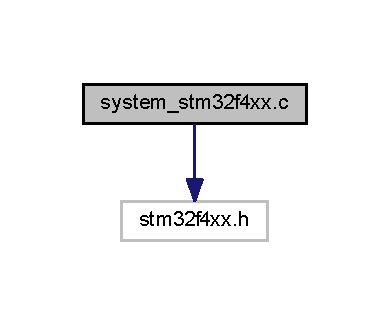
\includegraphics[width=187pt]{system__stm32f4xx_8c__incl}
\end{center}
\end{figure}
\subsection*{Macros}
\begin{DoxyCompactItemize}
\item 
\#define \mbox{\hyperlink{group___s_t_m32_f4xx___system___private___includes_gaeafcff4f57440c60e64812dddd13e7cb}{H\+S\+E\+\_\+\+V\+A\+L\+UE}}~((uint32\+\_\+t)25000000)
\item 
\#define \mbox{\hyperlink{group___s_t_m32_f4xx___system___private___includes_gaaa8c76e274d0f6dd2cefb5d0b17fbc37}{H\+S\+I\+\_\+\+V\+A\+L\+UE}}~((uint32\+\_\+t)16000000)
\item 
\#define \mbox{\hyperlink{group___s_t_m32_f4xx___system___private___defines_ga40e1495541cbb4acbe3f1819bd87a9fe}{V\+E\+C\+T\+\_\+\+T\+A\+B\+\_\+\+O\+F\+F\+S\+ET}}~0x00
\end{DoxyCompactItemize}
\subsection*{Functions}
\begin{DoxyCompactItemize}
\item 
void \mbox{\hyperlink{group___s_t_m32_f4xx___system___private___functions_ga93f514700ccf00d08dbdcff7f1224eb2}{System\+Init}} (void)
\begin{DoxyCompactList}\small\item\em Setup the microcontroller system Initialize the F\+PU setting, vector table location and External memory configuration. \end{DoxyCompactList}\item 
void \mbox{\hyperlink{group___s_t_m32_f4xx___system___private___functions_gae0c36a9591fe6e9c45ecb21a794f0f0f}{System\+Core\+Clock\+Update}} (void)
\begin{DoxyCompactList}\small\item\em Update System\+Core\+Clock variable according to Clock Register Values. The System\+Core\+Clock variable contains the core clock (H\+C\+LK), it can be used by the user application to setup the Sys\+Tick timer or configure other parameters. \end{DoxyCompactList}\end{DoxyCompactItemize}
\subsection*{Variables}
\begin{DoxyCompactItemize}
\item 
uint32\+\_\+t \mbox{\hyperlink{group___s_t_m32_f4xx___system___private___variables_gaa3cd3e43291e81e795d642b79b6088e6}{System\+Core\+Clock}} = 16000000
\item 
const uint8\+\_\+t \mbox{\hyperlink{group___s_t_m32_f4xx___system___private___variables_ga6e1d9cd666f0eacbfde31e9932a93466}{A\+H\+B\+Presc\+Table}} \mbox{[}16\mbox{]} = \{0, 0, 0, 0, 0, 0, 0, 0, 1, 2, 3, 4, 6, 7, 8, 9\}
\item 
const uint8\+\_\+t \mbox{\hyperlink{group___s_t_m32_f4xx___system___private___variables_ga5b4f8b768465842cf854a8f993b375e9}{A\+P\+B\+Presc\+Table}} \mbox{[}8\mbox{]} = \{0, 0, 0, 0, 1, 2, 3, 4\}
\end{DoxyCompactItemize}


\subsection{Detailed Description}
C\+M\+S\+IS Cortex-\/\+M4 Device Peripheral Access Layer System Source File. 

\begin{DoxyAuthor}{Author}
M\+CD Application Team This file provides two functions and one global variable to be called from user application\+:
\begin{DoxyItemize}
\item \mbox{\hyperlink{group___s_t_m32_f4xx___system___private___functions_ga93f514700ccf00d08dbdcff7f1224eb2}{System\+Init()}}\+: This function is called at startup just after reset and before branch to main program. This call is made inside the \char`\"{}startup\+\_\+stm32f4xx.\+s\char`\"{} file.
\item System\+Core\+Clock variable\+: Contains the core clock (H\+C\+LK), it can be used by the user application to setup the Sys\+Tick timer or configure other parameters.
\item \mbox{\hyperlink{group___s_t_m32_f4xx___system___private___functions_gae0c36a9591fe6e9c45ecb21a794f0f0f}{System\+Core\+Clock\+Update()}}\+: Updates the variable System\+Core\+Clock and must be called whenever the core clock is changed during program execution.
\end{DoxyItemize}
\end{DoxyAuthor}
\begin{DoxyAttention}{Attention}

\end{DoxyAttention}
\subsubsection*{\begin{center}\copyright{} C\+O\+P\+Y\+R\+I\+G\+HT 2017 S\+T\+Microelectronics\end{center} }

Redistribution and use in source and binary forms, with or without modification, are permitted provided that the following conditions are met\+:
\begin{DoxyEnumerate}
\item Redistributions of source code must retain the above copyright notice, this list of conditions and the following disclaimer.
\item Redistributions in binary form must reproduce the above copyright notice, this list of conditions and the following disclaimer in the documentation and/or other materials provided with the distribution.
\item Neither the name of S\+T\+Microelectronics nor the names of its contributors may be used to endorse or promote products derived from this software without specific prior written permission.
\end{DoxyEnumerate}

T\+H\+IS S\+O\+F\+T\+W\+A\+RE IS P\+R\+O\+V\+I\+D\+ED BY T\+HE C\+O\+P\+Y\+R\+I\+G\+HT H\+O\+L\+D\+E\+RS A\+ND C\+O\+N\+T\+R\+I\+B\+U\+T\+O\+RS \char`\"{}\+A\+S I\+S\char`\"{} A\+ND A\+NY E\+X\+P\+R\+E\+SS OR I\+M\+P\+L\+I\+ED W\+A\+R\+R\+A\+N\+T\+I\+ES, I\+N\+C\+L\+U\+D\+I\+NG, B\+UT N\+OT L\+I\+M\+I\+T\+ED TO, T\+HE I\+M\+P\+L\+I\+ED W\+A\+R\+R\+A\+N\+T\+I\+ES OF M\+E\+R\+C\+H\+A\+N\+T\+A\+B\+I\+L\+I\+TY A\+ND F\+I\+T\+N\+E\+SS F\+OR A P\+A\+R\+T\+I\+C\+U\+L\+AR P\+U\+R\+P\+O\+SE A\+RE D\+I\+S\+C\+L\+A\+I\+M\+ED. IN NO E\+V\+E\+NT S\+H\+A\+LL T\+HE C\+O\+P\+Y\+R\+I\+G\+HT H\+O\+L\+D\+ER OR C\+O\+N\+T\+R\+I\+B\+U\+T\+O\+RS BE L\+I\+A\+B\+LE F\+OR A\+NY D\+I\+R\+E\+CT, I\+N\+D\+I\+R\+E\+CT, I\+N\+C\+I\+D\+E\+N\+T\+AL, S\+P\+E\+C\+I\+AL, E\+X\+E\+M\+P\+L\+A\+RY, OR C\+O\+N\+S\+E\+Q\+U\+E\+N\+T\+I\+AL D\+A\+M\+A\+G\+ES (I\+N\+C\+L\+U\+D\+I\+NG, B\+UT N\+OT L\+I\+M\+I\+T\+ED TO, P\+R\+O\+C\+U\+R\+E\+M\+E\+NT OF S\+U\+B\+S\+T\+I\+T\+U\+TE G\+O\+O\+DS OR S\+E\+R\+V\+I\+C\+ES; L\+O\+SS OF U\+SE, D\+A\+TA, OR P\+R\+O\+F\+I\+TS; OR B\+U\+S\+I\+N\+E\+SS I\+N\+T\+E\+R\+R\+U\+P\+T\+I\+ON) H\+O\+W\+E\+V\+ER C\+A\+U\+S\+ED A\+ND ON A\+NY T\+H\+E\+O\+RY OF L\+I\+A\+B\+I\+L\+I\+TY, W\+H\+E\+T\+H\+ER IN C\+O\+N\+T\+R\+A\+CT, S\+T\+R\+I\+CT L\+I\+A\+B\+I\+L\+I\+TY, OR T\+O\+RT (I\+N\+C\+L\+U\+D\+I\+NG N\+E\+G\+L\+I\+G\+E\+N\+CE OR O\+T\+H\+E\+R\+W\+I\+SE) A\+R\+I\+S\+I\+NG IN A\+NY W\+AY O\+UT OF T\+HE U\+SE OF T\+H\+IS S\+O\+F\+T\+W\+A\+RE, E\+V\+EN IF A\+D\+V\+I\+S\+ED OF T\+HE P\+O\+S\+S\+I\+B\+I\+L\+I\+TY OF S\+U\+CH D\+A\+M\+A\+GE. 
\hypertarget{tim_8c}{}\section{tim.\+c File Reference}
\label{tim_8c}\index{tim.\+c@{tim.\+c}}
{\ttfamily \#include \char`\"{}tim.\+h\char`\"{}}\newline
Include dependency graph for tim.\+c\+:
\nopagebreak
\begin{figure}[H]
\begin{center}
\leavevmode
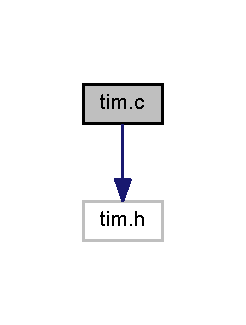
\includegraphics[width=118pt]{tim_8c__incl}
\end{center}
\end{figure}
\subsection*{Functions}
\begin{DoxyCompactItemize}
\item 
void \mbox{\hyperlink{tim_8c_a7912f2916786a2c33cb6fb8259ade58c}{M\+X\+\_\+\+T\+I\+M3\+\_\+\+Init}} (void)
\item 
void \mbox{\hyperlink{tim_8c_a5ee937d52485d5cda27896e3842a7ca1}{M\+X\+\_\+\+T\+I\+M5\+\_\+\+Init}} (void)
\item 
void \mbox{\hyperlink{tim_8c_a59716af159bfbbb6023b31354fb23af8}{H\+A\+L\+\_\+\+T\+I\+M\+\_\+\+Base\+\_\+\+Msp\+Init}} (T\+I\+M\+\_\+\+Handle\+Type\+Def $\ast$tim\+\_\+base\+Handle)
\item 
void \mbox{\hyperlink{tim_8c_a708f19bbc41b292fccf38f2d9796c46a}{H\+A\+L\+\_\+\+T\+I\+M\+\_\+\+Msp\+Post\+Init}} (T\+I\+M\+\_\+\+Handle\+Type\+Def $\ast$tim\+Handle)
\item 
void \mbox{\hyperlink{tim_8c_adee8ed7d3ebb3a217c27ac10af86ce2f}{H\+A\+L\+\_\+\+T\+I\+M\+\_\+\+Base\+\_\+\+Msp\+De\+Init}} (T\+I\+M\+\_\+\+Handle\+Type\+Def $\ast$tim\+\_\+base\+Handle)
\end{DoxyCompactItemize}
\subsection*{Variables}
\begin{DoxyCompactItemize}
\item 
T\+I\+M\+\_\+\+Handle\+Type\+Def \mbox{\hyperlink{tim_8c_aac3d2c59ee0e3bbae1b99529a154eb62}{htim3}}
\item 
T\+I\+M\+\_\+\+Handle\+Type\+Def \mbox{\hyperlink{tim_8c_acefaeaaa3856ddddae7083b2d220fe4b}{htim5}}
\end{DoxyCompactItemize}


\subsection{Function Documentation}
\mbox{\Hypertarget{tim_8c_adee8ed7d3ebb3a217c27ac10af86ce2f}\label{tim_8c_adee8ed7d3ebb3a217c27ac10af86ce2f}} 
\index{tim.\+c@{tim.\+c}!H\+A\+L\+\_\+\+T\+I\+M\+\_\+\+Base\+\_\+\+Msp\+De\+Init@{H\+A\+L\+\_\+\+T\+I\+M\+\_\+\+Base\+\_\+\+Msp\+De\+Init}}
\index{H\+A\+L\+\_\+\+T\+I\+M\+\_\+\+Base\+\_\+\+Msp\+De\+Init@{H\+A\+L\+\_\+\+T\+I\+M\+\_\+\+Base\+\_\+\+Msp\+De\+Init}!tim.\+c@{tim.\+c}}
\subsubsection{\texorpdfstring{H\+A\+L\+\_\+\+T\+I\+M\+\_\+\+Base\+\_\+\+Msp\+De\+Init()}{HAL\_TIM\_Base\_MspDeInit()}}
{\footnotesize\ttfamily void H\+A\+L\+\_\+\+T\+I\+M\+\_\+\+Base\+\_\+\+Msp\+De\+Init (\begin{DoxyParamCaption}\item[{T\+I\+M\+\_\+\+Handle\+Type\+Def $\ast$}]{tim\+\_\+base\+Handle }\end{DoxyParamCaption})}



Definition at line 235 of file tim.\+c.

\mbox{\Hypertarget{tim_8c_a59716af159bfbbb6023b31354fb23af8}\label{tim_8c_a59716af159bfbbb6023b31354fb23af8}} 
\index{tim.\+c@{tim.\+c}!H\+A\+L\+\_\+\+T\+I\+M\+\_\+\+Base\+\_\+\+Msp\+Init@{H\+A\+L\+\_\+\+T\+I\+M\+\_\+\+Base\+\_\+\+Msp\+Init}}
\index{H\+A\+L\+\_\+\+T\+I\+M\+\_\+\+Base\+\_\+\+Msp\+Init@{H\+A\+L\+\_\+\+T\+I\+M\+\_\+\+Base\+\_\+\+Msp\+Init}!tim.\+c@{tim.\+c}}
\subsubsection{\texorpdfstring{H\+A\+L\+\_\+\+T\+I\+M\+\_\+\+Base\+\_\+\+Msp\+Init()}{HAL\_TIM\_Base\_MspInit()}}
{\footnotesize\ttfamily void H\+A\+L\+\_\+\+T\+I\+M\+\_\+\+Base\+\_\+\+Msp\+Init (\begin{DoxyParamCaption}\item[{T\+I\+M\+\_\+\+Handle\+Type\+Def $\ast$}]{tim\+\_\+base\+Handle }\end{DoxyParamCaption})}



Definition at line 155 of file tim.\+c.

\mbox{\Hypertarget{tim_8c_a708f19bbc41b292fccf38f2d9796c46a}\label{tim_8c_a708f19bbc41b292fccf38f2d9796c46a}} 
\index{tim.\+c@{tim.\+c}!H\+A\+L\+\_\+\+T\+I\+M\+\_\+\+Msp\+Post\+Init@{H\+A\+L\+\_\+\+T\+I\+M\+\_\+\+Msp\+Post\+Init}}
\index{H\+A\+L\+\_\+\+T\+I\+M\+\_\+\+Msp\+Post\+Init@{H\+A\+L\+\_\+\+T\+I\+M\+\_\+\+Msp\+Post\+Init}!tim.\+c@{tim.\+c}}
\subsubsection{\texorpdfstring{H\+A\+L\+\_\+\+T\+I\+M\+\_\+\+Msp\+Post\+Init()}{HAL\_TIM\_MspPostInit()}}
{\footnotesize\ttfamily void H\+A\+L\+\_\+\+T\+I\+M\+\_\+\+Msp\+Post\+Init (\begin{DoxyParamCaption}\item[{T\+I\+M\+\_\+\+Handle\+Type\+Def $\ast$}]{tim\+Handle }\end{DoxyParamCaption})}

T\+I\+M3 G\+P\+IO Configuration ~\newline
~\newline
P\+B4 ------$>$ T\+I\+M3\+\_\+\+C\+H1

T\+I\+M5 G\+P\+IO Configuration ~\newline
P\+A0-\/\+W\+K\+UP -\/-\/-\/---$>$ T\+I\+M5\+\_\+\+C\+H1

Definition at line 189 of file tim.\+c.

Here is the caller graph for this function\+:
\nopagebreak
\begin{figure}[H]
\begin{center}
\leavevmode
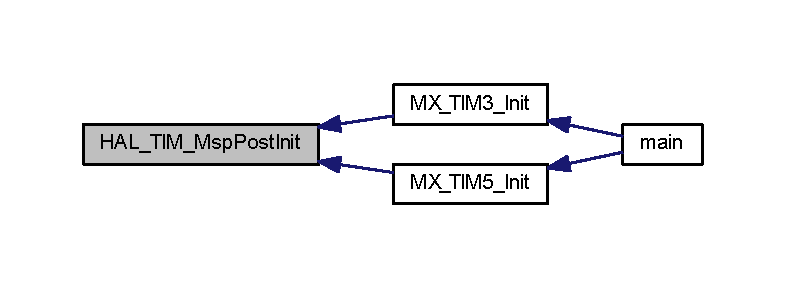
\includegraphics[width=350pt]{tim_8c_a708f19bbc41b292fccf38f2d9796c46a_icgraph}
\end{center}
\end{figure}
\mbox{\Hypertarget{tim_8c_a7912f2916786a2c33cb6fb8259ade58c}\label{tim_8c_a7912f2916786a2c33cb6fb8259ade58c}} 
\index{tim.\+c@{tim.\+c}!M\+X\+\_\+\+T\+I\+M3\+\_\+\+Init@{M\+X\+\_\+\+T\+I\+M3\+\_\+\+Init}}
\index{M\+X\+\_\+\+T\+I\+M3\+\_\+\+Init@{M\+X\+\_\+\+T\+I\+M3\+\_\+\+Init}!tim.\+c@{tim.\+c}}
\subsubsection{\texorpdfstring{M\+X\+\_\+\+T\+I\+M3\+\_\+\+Init()}{MX\_TIM3\_Init()}}
{\footnotesize\ttfamily void M\+X\+\_\+\+T\+I\+M3\+\_\+\+Init (\begin{DoxyParamCaption}\item[{void}]{ }\end{DoxyParamCaption})}



Definition at line 61 of file tim.\+c.

Here is the call graph for this function\+:
\nopagebreak
\begin{figure}[H]
\begin{center}
\leavevmode
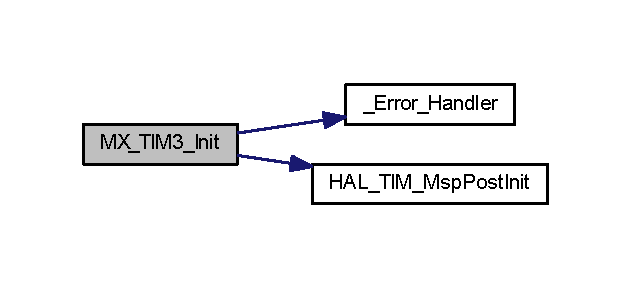
\includegraphics[width=303pt]{tim_8c_a7912f2916786a2c33cb6fb8259ade58c_cgraph}
\end{center}
\end{figure}
Here is the caller graph for this function\+:
\nopagebreak
\begin{figure}[H]
\begin{center}
\leavevmode
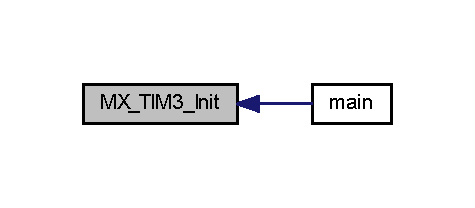
\includegraphics[width=228pt]{tim_8c_a7912f2916786a2c33cb6fb8259ade58c_icgraph}
\end{center}
\end{figure}
\mbox{\Hypertarget{tim_8c_a5ee937d52485d5cda27896e3842a7ca1}\label{tim_8c_a5ee937d52485d5cda27896e3842a7ca1}} 
\index{tim.\+c@{tim.\+c}!M\+X\+\_\+\+T\+I\+M5\+\_\+\+Init@{M\+X\+\_\+\+T\+I\+M5\+\_\+\+Init}}
\index{M\+X\+\_\+\+T\+I\+M5\+\_\+\+Init@{M\+X\+\_\+\+T\+I\+M5\+\_\+\+Init}!tim.\+c@{tim.\+c}}
\subsubsection{\texorpdfstring{M\+X\+\_\+\+T\+I\+M5\+\_\+\+Init()}{MX\_TIM5\_Init()}}
{\footnotesize\ttfamily void M\+X\+\_\+\+T\+I\+M5\+\_\+\+Init (\begin{DoxyParamCaption}\item[{void}]{ }\end{DoxyParamCaption})}



Definition at line 108 of file tim.\+c.

Here is the call graph for this function\+:
\nopagebreak
\begin{figure}[H]
\begin{center}
\leavevmode
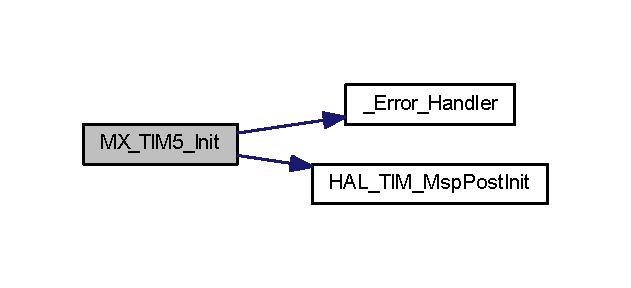
\includegraphics[width=303pt]{tim_8c_a5ee937d52485d5cda27896e3842a7ca1_cgraph}
\end{center}
\end{figure}
Here is the caller graph for this function\+:
\nopagebreak
\begin{figure}[H]
\begin{center}
\leavevmode
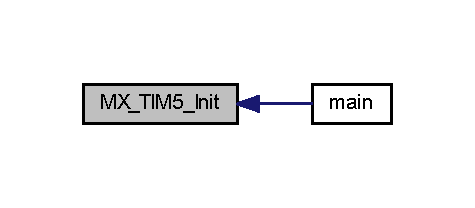
\includegraphics[width=228pt]{tim_8c_a5ee937d52485d5cda27896e3842a7ca1_icgraph}
\end{center}
\end{figure}


\subsection{Variable Documentation}
\mbox{\Hypertarget{tim_8c_aac3d2c59ee0e3bbae1b99529a154eb62}\label{tim_8c_aac3d2c59ee0e3bbae1b99529a154eb62}} 
\index{tim.\+c@{tim.\+c}!htim3@{htim3}}
\index{htim3@{htim3}!tim.\+c@{tim.\+c}}
\subsubsection{\texorpdfstring{htim3}{htim3}}
{\footnotesize\ttfamily T\+I\+M\+\_\+\+Handle\+Type\+Def htim3}

File Name \+: \mbox{\hyperlink{tim_8c}{T\+I\+M.\+c}} Description \+: This file provides code for the configuration of the T\+IM instances.

This notice applies to any and all portions of this file that are not between comment pairs U\+S\+ER C\+O\+DE B\+E\+G\+IN and U\+S\+ER C\+O\+DE E\+ND. Other portions of this file, whether inserted by the user or by software development tools are owned by their respective copyright owners.

Copyright (c) 2018 S\+T\+Microelectronics International N.\+V. All rights reserved.

Redistribution and use in source and binary forms, with or without modification, are permitted, provided that the following conditions are met\+:


\begin{DoxyEnumerate}
\item Redistribution of source code must retain the above copyright notice, this list of conditions and the following disclaimer.
\item Redistributions in binary form must reproduce the above copyright notice, this list of conditions and the following disclaimer in the documentation and/or other materials provided with the distribution.
\item Neither the name of S\+T\+Microelectronics nor the names of other contributors to this software may be used to endorse or promote products derived from this software without specific written permission.
\item This software, including modifications and/or derivative works of this software, must execute solely and exclusively on microcontroller or microprocessor devices manufactured by or for S\+T\+Microelectronics.
\item Redistribution and use of this software other than as permitted under this license is void and will automatically terminate your rights under this license.
\end{DoxyEnumerate}

T\+H\+IS S\+O\+F\+T\+W\+A\+RE IS P\+R\+O\+V\+I\+D\+ED BY S\+T\+M\+I\+C\+R\+O\+E\+L\+E\+C\+T\+R\+O\+N\+I\+CS A\+ND C\+O\+N\+T\+R\+I\+B\+U\+T\+O\+RS \char`\"{}\+A\+S I\+S\char`\"{} A\+ND A\+NY E\+X\+P\+R\+E\+SS, I\+M\+P\+L\+I\+ED OR S\+T\+A\+T\+U\+T\+O\+RY W\+A\+R\+R\+A\+N\+T\+I\+ES, I\+N\+C\+L\+U\+D\+I\+NG, B\+UT N\+OT L\+I\+M\+I\+T\+ED TO, T\+HE I\+M\+P\+L\+I\+ED W\+A\+R\+R\+A\+N\+T\+I\+ES OF M\+E\+R\+C\+H\+A\+N\+T\+A\+B\+I\+L\+I\+TY, F\+I\+T\+N\+E\+SS F\+OR A P\+A\+R\+T\+I\+C\+U\+L\+AR P\+U\+R\+P\+O\+SE A\+ND N\+O\+N-\/\+I\+N\+F\+R\+I\+N\+G\+E\+M\+E\+NT OF T\+H\+I\+RD P\+A\+R\+TY I\+N\+T\+E\+L\+L\+E\+C\+T\+U\+AL P\+R\+O\+P\+E\+R\+TY R\+I\+G\+H\+TS A\+RE D\+I\+S\+C\+L\+A\+I\+M\+ED TO T\+HE F\+U\+L\+L\+E\+ST E\+X\+T\+E\+NT P\+E\+R\+M\+I\+T\+T\+ED BY L\+AW. IN NO E\+V\+E\+NT S\+H\+A\+LL S\+T\+M\+I\+C\+R\+O\+E\+L\+E\+C\+T\+R\+O\+N\+I\+CS OR C\+O\+N\+T\+R\+I\+B\+U\+T\+O\+RS BE L\+I\+A\+B\+LE F\+OR A\+NY D\+I\+R\+E\+CT, I\+N\+D\+I\+R\+E\+CT, I\+N\+C\+I\+D\+E\+N\+T\+AL, S\+P\+E\+C\+I\+AL, E\+X\+E\+M\+P\+L\+A\+RY, OR C\+O\+N\+S\+E\+Q\+U\+E\+N\+T\+I\+AL D\+A\+M\+A\+G\+ES (I\+N\+C\+L\+U\+D\+I\+NG, B\+UT N\+OT L\+I\+M\+I\+T\+ED TO, P\+R\+O\+C\+U\+R\+E\+M\+E\+NT OF S\+U\+B\+S\+T\+I\+T\+U\+TE G\+O\+O\+DS OR S\+E\+R\+V\+I\+C\+ES; L\+O\+SS OF U\+SE, D\+A\+TA, OR P\+R\+O\+F\+I\+TS; OR B\+U\+S\+I\+N\+E\+SS I\+N\+T\+E\+R\+R\+U\+P\+T\+I\+ON) H\+O\+W\+E\+V\+ER C\+A\+U\+S\+ED A\+ND ON A\+NY T\+H\+E\+O\+RY OF L\+I\+A\+B\+I\+L\+I\+TY, W\+H\+E\+T\+H\+ER IN C\+O\+N\+T\+R\+A\+CT, S\+T\+R\+I\+CT L\+I\+A\+B\+I\+L\+I\+TY, OR T\+O\+RT (I\+N\+C\+L\+U\+D\+I\+NG N\+E\+G\+L\+I\+G\+E\+N\+CE OR O\+T\+H\+E\+R\+W\+I\+SE) A\+R\+I\+S\+I\+NG IN A\+NY W\+AY O\+UT OF T\+HE U\+SE OF T\+H\+IS S\+O\+F\+T\+W\+A\+RE, E\+V\+EN IF A\+D\+V\+I\+S\+ED OF T\+HE P\+O\+S\+S\+I\+B\+I\+L\+I\+TY OF S\+U\+CH D\+A\+M\+A\+GE. 

Definition at line 57 of file tim.\+c.

\mbox{\Hypertarget{tim_8c_acefaeaaa3856ddddae7083b2d220fe4b}\label{tim_8c_acefaeaaa3856ddddae7083b2d220fe4b}} 
\index{tim.\+c@{tim.\+c}!htim5@{htim5}}
\index{htim5@{htim5}!tim.\+c@{tim.\+c}}
\subsubsection{\texorpdfstring{htim5}{htim5}}
{\footnotesize\ttfamily T\+I\+M\+\_\+\+Handle\+Type\+Def htim5}



Definition at line 58 of file tim.\+c.


\hypertarget{usart_8c}{}\section{usart.\+c File Reference}
\label{usart_8c}\index{usart.\+c@{usart.\+c}}
{\ttfamily \#include \char`\"{}usart.\+h\char`\"{}}\newline
{\ttfamily \#include \char`\"{}gpio.\+h\char`\"{}}\newline
{\ttfamily \#include \char`\"{}dma.\+h\char`\"{}}\newline
Include dependency graph for usart.\+c\+:
\nopagebreak
\begin{figure}[H]
\begin{center}
\leavevmode
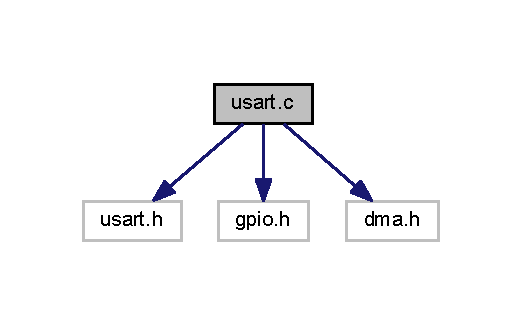
\includegraphics[width=251pt]{usart_8c__incl}
\end{center}
\end{figure}
\subsection*{Functions}
\begin{DoxyCompactItemize}
\item 
void \mbox{\hyperlink{usart_8c_a052088fe5bb3f807a4b2502e664fd4fd}{M\+X\+\_\+\+U\+S\+A\+R\+T2\+\_\+\+U\+A\+R\+T\+\_\+\+Init}} (void)
\item 
void \mbox{\hyperlink{usart_8c_a62a25476866998c7aadfb5c0864fa349}{H\+A\+L\+\_\+\+U\+A\+R\+T\+\_\+\+Msp\+Init}} (U\+A\+R\+T\+\_\+\+Handle\+Type\+Def $\ast$uart\+Handle)
\item 
void \mbox{\hyperlink{usart_8c_a94cd2c58add4f2549895a03bf267622e}{H\+A\+L\+\_\+\+U\+A\+R\+T\+\_\+\+Msp\+De\+Init}} (U\+A\+R\+T\+\_\+\+Handle\+Type\+Def $\ast$uart\+Handle)
\end{DoxyCompactItemize}
\subsection*{Variables}
\begin{DoxyCompactItemize}
\item 
U\+A\+R\+T\+\_\+\+Handle\+Type\+Def \mbox{\hyperlink{usart_8c_aa9479c261d65eecedd3d9582f7f0f89c}{huart2}}
\item 
D\+M\+A\+\_\+\+Handle\+Type\+Def \mbox{\hyperlink{usart_8c_a0083b476c2a75ab9fb2ccbed0048857e}{hdma\+\_\+usart2\+\_\+tx}}
\item 
D\+M\+A\+\_\+\+Handle\+Type\+Def \mbox{\hyperlink{usart_8c_a784aa25dc7e4580cfbf80658340f482c}{hdma\+\_\+usart2\+\_\+rx}}
\end{DoxyCompactItemize}


\subsection{Function Documentation}
\mbox{\Hypertarget{usart_8c_a94cd2c58add4f2549895a03bf267622e}\label{usart_8c_a94cd2c58add4f2549895a03bf267622e}} 
\index{usart.\+c@{usart.\+c}!H\+A\+L\+\_\+\+U\+A\+R\+T\+\_\+\+Msp\+De\+Init@{H\+A\+L\+\_\+\+U\+A\+R\+T\+\_\+\+Msp\+De\+Init}}
\index{H\+A\+L\+\_\+\+U\+A\+R\+T\+\_\+\+Msp\+De\+Init@{H\+A\+L\+\_\+\+U\+A\+R\+T\+\_\+\+Msp\+De\+Init}!usart.\+c@{usart.\+c}}
\subsubsection{\texorpdfstring{H\+A\+L\+\_\+\+U\+A\+R\+T\+\_\+\+Msp\+De\+Init()}{HAL\_UART\_MspDeInit()}}
{\footnotesize\ttfamily void H\+A\+L\+\_\+\+U\+A\+R\+T\+\_\+\+Msp\+De\+Init (\begin{DoxyParamCaption}\item[{U\+A\+R\+T\+\_\+\+Handle\+Type\+Def $\ast$}]{uart\+Handle }\end{DoxyParamCaption})}

U\+S\+A\+R\+T2 G\+P\+IO Configuration ~\newline
P\+A2 -\/-\/-\/---$>$ U\+S\+A\+R\+T2\+\_\+\+TX P\+A3 -\/-\/-\/---$>$ U\+S\+A\+R\+T2\+\_\+\+RX

Definition at line 154 of file usart.\+c.

\mbox{\Hypertarget{usart_8c_a62a25476866998c7aadfb5c0864fa349}\label{usart_8c_a62a25476866998c7aadfb5c0864fa349}} 
\index{usart.\+c@{usart.\+c}!H\+A\+L\+\_\+\+U\+A\+R\+T\+\_\+\+Msp\+Init@{H\+A\+L\+\_\+\+U\+A\+R\+T\+\_\+\+Msp\+Init}}
\index{H\+A\+L\+\_\+\+U\+A\+R\+T\+\_\+\+Msp\+Init@{H\+A\+L\+\_\+\+U\+A\+R\+T\+\_\+\+Msp\+Init}!usart.\+c@{usart.\+c}}
\subsubsection{\texorpdfstring{H\+A\+L\+\_\+\+U\+A\+R\+T\+\_\+\+Msp\+Init()}{HAL\_UART\_MspInit()}}
{\footnotesize\ttfamily void H\+A\+L\+\_\+\+U\+A\+R\+T\+\_\+\+Msp\+Init (\begin{DoxyParamCaption}\item[{U\+A\+R\+T\+\_\+\+Handle\+Type\+Def $\ast$}]{uart\+Handle }\end{DoxyParamCaption})}

U\+S\+A\+R\+T2 G\+P\+IO Configuration ~\newline
P\+A2 -\/-\/-\/---$>$ U\+S\+A\+R\+T2\+\_\+\+TX P\+A3 -\/-\/-\/---$>$ U\+S\+A\+R\+T2\+\_\+\+RX

Definition at line 84 of file usart.\+c.

Here is the call graph for this function\+:
\nopagebreak
\begin{figure}[H]
\begin{center}
\leavevmode
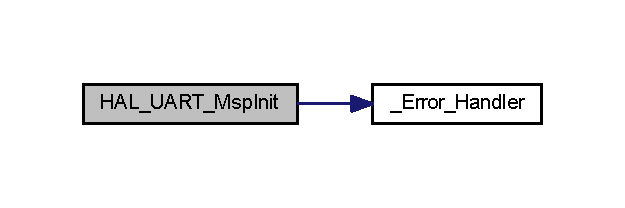
\includegraphics[width=300pt]{usart_8c_a62a25476866998c7aadfb5c0864fa349_cgraph}
\end{center}
\end{figure}
\mbox{\Hypertarget{usart_8c_a052088fe5bb3f807a4b2502e664fd4fd}\label{usart_8c_a052088fe5bb3f807a4b2502e664fd4fd}} 
\index{usart.\+c@{usart.\+c}!M\+X\+\_\+\+U\+S\+A\+R\+T2\+\_\+\+U\+A\+R\+T\+\_\+\+Init@{M\+X\+\_\+\+U\+S\+A\+R\+T2\+\_\+\+U\+A\+R\+T\+\_\+\+Init}}
\index{M\+X\+\_\+\+U\+S\+A\+R\+T2\+\_\+\+U\+A\+R\+T\+\_\+\+Init@{M\+X\+\_\+\+U\+S\+A\+R\+T2\+\_\+\+U\+A\+R\+T\+\_\+\+Init}!usart.\+c@{usart.\+c}}
\subsubsection{\texorpdfstring{M\+X\+\_\+\+U\+S\+A\+R\+T2\+\_\+\+U\+A\+R\+T\+\_\+\+Init()}{MX\_USART2\_UART\_Init()}}
{\footnotesize\ttfamily void M\+X\+\_\+\+U\+S\+A\+R\+T2\+\_\+\+U\+A\+R\+T\+\_\+\+Init (\begin{DoxyParamCaption}\item[{void}]{ }\end{DoxyParamCaption})}



Definition at line 66 of file usart.\+c.

Here is the call graph for this function\+:
\nopagebreak
\begin{figure}[H]
\begin{center}
\leavevmode
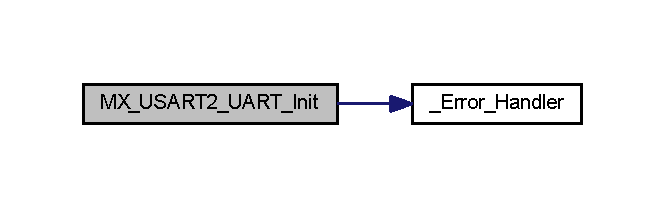
\includegraphics[width=319pt]{usart_8c_a052088fe5bb3f807a4b2502e664fd4fd_cgraph}
\end{center}
\end{figure}
Here is the caller graph for this function\+:
\nopagebreak
\begin{figure}[H]
\begin{center}
\leavevmode
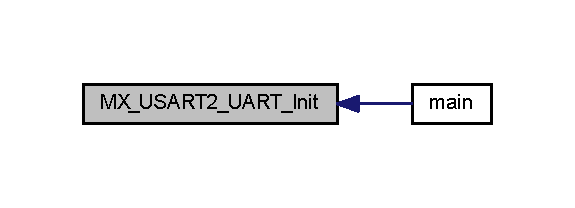
\includegraphics[width=276pt]{usart_8c_a052088fe5bb3f807a4b2502e664fd4fd_icgraph}
\end{center}
\end{figure}


\subsection{Variable Documentation}
\mbox{\Hypertarget{usart_8c_a784aa25dc7e4580cfbf80658340f482c}\label{usart_8c_a784aa25dc7e4580cfbf80658340f482c}} 
\index{usart.\+c@{usart.\+c}!hdma\+\_\+usart2\+\_\+rx@{hdma\+\_\+usart2\+\_\+rx}}
\index{hdma\+\_\+usart2\+\_\+rx@{hdma\+\_\+usart2\+\_\+rx}!usart.\+c@{usart.\+c}}
\subsubsection{\texorpdfstring{hdma\+\_\+usart2\+\_\+rx}{hdma\_usart2\_rx}}
{\footnotesize\ttfamily D\+M\+A\+\_\+\+Handle\+Type\+Def hdma\+\_\+usart2\+\_\+rx}



Definition at line 62 of file usart.\+c.

\mbox{\Hypertarget{usart_8c_a0083b476c2a75ab9fb2ccbed0048857e}\label{usart_8c_a0083b476c2a75ab9fb2ccbed0048857e}} 
\index{usart.\+c@{usart.\+c}!hdma\+\_\+usart2\+\_\+tx@{hdma\+\_\+usart2\+\_\+tx}}
\index{hdma\+\_\+usart2\+\_\+tx@{hdma\+\_\+usart2\+\_\+tx}!usart.\+c@{usart.\+c}}
\subsubsection{\texorpdfstring{hdma\+\_\+usart2\+\_\+tx}{hdma\_usart2\_tx}}
{\footnotesize\ttfamily D\+M\+A\+\_\+\+Handle\+Type\+Def hdma\+\_\+usart2\+\_\+tx}



Definition at line 61 of file usart.\+c.

\mbox{\Hypertarget{usart_8c_aa9479c261d65eecedd3d9582f7f0f89c}\label{usart_8c_aa9479c261d65eecedd3d9582f7f0f89c}} 
\index{usart.\+c@{usart.\+c}!huart2@{huart2}}
\index{huart2@{huart2}!usart.\+c@{usart.\+c}}
\subsubsection{\texorpdfstring{huart2}{huart2}}
{\footnotesize\ttfamily U\+A\+R\+T\+\_\+\+Handle\+Type\+Def huart2}

File Name \+: \mbox{\hyperlink{usart_8c}{U\+S\+A\+R\+T.\+c}} Description \+: This file provides code for the configuration of the U\+S\+A\+RT instances.

This notice applies to any and all portions of this file that are not between comment pairs U\+S\+ER C\+O\+DE B\+E\+G\+IN and U\+S\+ER C\+O\+DE E\+ND. Other portions of this file, whether inserted by the user or by software development tools are owned by their respective copyright owners.

Copyright (c) 2018 S\+T\+Microelectronics International N.\+V. All rights reserved.

Redistribution and use in source and binary forms, with or without modification, are permitted, provided that the following conditions are met\+:


\begin{DoxyEnumerate}
\item Redistribution of source code must retain the above copyright notice, this list of conditions and the following disclaimer.
\item Redistributions in binary form must reproduce the above copyright notice, this list of conditions and the following disclaimer in the documentation and/or other materials provided with the distribution.
\item Neither the name of S\+T\+Microelectronics nor the names of other contributors to this software may be used to endorse or promote products derived from this software without specific written permission.
\item This software, including modifications and/or derivative works of this software, must execute solely and exclusively on microcontroller or microprocessor devices manufactured by or for S\+T\+Microelectronics.
\item Redistribution and use of this software other than as permitted under this license is void and will automatically terminate your rights under this license.
\end{DoxyEnumerate}

T\+H\+IS S\+O\+F\+T\+W\+A\+RE IS P\+R\+O\+V\+I\+D\+ED BY S\+T\+M\+I\+C\+R\+O\+E\+L\+E\+C\+T\+R\+O\+N\+I\+CS A\+ND C\+O\+N\+T\+R\+I\+B\+U\+T\+O\+RS \char`\"{}\+A\+S I\+S\char`\"{} A\+ND A\+NY E\+X\+P\+R\+E\+SS, I\+M\+P\+L\+I\+ED OR S\+T\+A\+T\+U\+T\+O\+RY W\+A\+R\+R\+A\+N\+T\+I\+ES, I\+N\+C\+L\+U\+D\+I\+NG, B\+UT N\+OT L\+I\+M\+I\+T\+ED TO, T\+HE I\+M\+P\+L\+I\+ED W\+A\+R\+R\+A\+N\+T\+I\+ES OF M\+E\+R\+C\+H\+A\+N\+T\+A\+B\+I\+L\+I\+TY, F\+I\+T\+N\+E\+SS F\+OR A P\+A\+R\+T\+I\+C\+U\+L\+AR P\+U\+R\+P\+O\+SE A\+ND N\+O\+N-\/\+I\+N\+F\+R\+I\+N\+G\+E\+M\+E\+NT OF T\+H\+I\+RD P\+A\+R\+TY I\+N\+T\+E\+L\+L\+E\+C\+T\+U\+AL P\+R\+O\+P\+E\+R\+TY R\+I\+G\+H\+TS A\+RE D\+I\+S\+C\+L\+A\+I\+M\+ED TO T\+HE F\+U\+L\+L\+E\+ST E\+X\+T\+E\+NT P\+E\+R\+M\+I\+T\+T\+ED BY L\+AW. IN NO E\+V\+E\+NT S\+H\+A\+LL S\+T\+M\+I\+C\+R\+O\+E\+L\+E\+C\+T\+R\+O\+N\+I\+CS OR C\+O\+N\+T\+R\+I\+B\+U\+T\+O\+RS BE L\+I\+A\+B\+LE F\+OR A\+NY D\+I\+R\+E\+CT, I\+N\+D\+I\+R\+E\+CT, I\+N\+C\+I\+D\+E\+N\+T\+AL, S\+P\+E\+C\+I\+AL, E\+X\+E\+M\+P\+L\+A\+RY, OR C\+O\+N\+S\+E\+Q\+U\+E\+N\+T\+I\+AL D\+A\+M\+A\+G\+ES (I\+N\+C\+L\+U\+D\+I\+NG, B\+UT N\+OT L\+I\+M\+I\+T\+ED TO, P\+R\+O\+C\+U\+R\+E\+M\+E\+NT OF S\+U\+B\+S\+T\+I\+T\+U\+TE G\+O\+O\+DS OR S\+E\+R\+V\+I\+C\+ES; L\+O\+SS OF U\+SE, D\+A\+TA, OR P\+R\+O\+F\+I\+TS; OR B\+U\+S\+I\+N\+E\+SS I\+N\+T\+E\+R\+R\+U\+P\+T\+I\+ON) H\+O\+W\+E\+V\+ER C\+A\+U\+S\+ED A\+ND ON A\+NY T\+H\+E\+O\+RY OF L\+I\+A\+B\+I\+L\+I\+TY, W\+H\+E\+T\+H\+ER IN C\+O\+N\+T\+R\+A\+CT, S\+T\+R\+I\+CT L\+I\+A\+B\+I\+L\+I\+TY, OR T\+O\+RT (I\+N\+C\+L\+U\+D\+I\+NG N\+E\+G\+L\+I\+G\+E\+N\+CE OR O\+T\+H\+E\+R\+W\+I\+SE) A\+R\+I\+S\+I\+NG IN A\+NY W\+AY O\+UT OF T\+HE U\+SE OF T\+H\+IS S\+O\+F\+T\+W\+A\+RE, E\+V\+EN IF A\+D\+V\+I\+S\+ED OF T\+HE P\+O\+S\+S\+I\+B\+I\+L\+I\+TY OF S\+U\+CH D\+A\+M\+A\+GE. 

Definition at line 60 of file usart.\+c.


\hypertarget{user__diskio_8c}{}\section{Src/user\+\_\+diskio.c File Reference}
\label{user__diskio_8c}\index{Src/user\+\_\+diskio.\+c@{Src/user\+\_\+diskio.\+c}}


This file includes a diskio driver skeleton to be completed by the user.  


{\ttfamily \#include $<$string.\+h$>$}\newline
{\ttfamily \#include \char`\"{}ff\+\_\+gen\+\_\+drv.\+h\char`\"{}}\newline
Include dependency graph for user\+\_\+diskio.\+c\+:\nopagebreak
\begin{figure}[H]
\begin{center}
\leavevmode
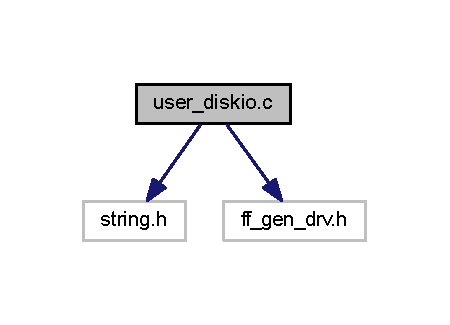
\includegraphics[width=216pt]{user__diskio_8c__incl}
\end{center}
\end{figure}
\subsection*{Functions}
\begin{DoxyCompactItemize}
\item 
D\+S\+T\+A\+T\+US \mbox{\hyperlink{user__diskio_8c_a525eefa6ed9c9fd5eb6194d78e120588}{U\+S\+E\+R\+\_\+initialize}} (B\+Y\+TE pdrv)
\begin{DoxyCompactList}\small\item\em Initializes a Drive. \end{DoxyCompactList}\item 
D\+S\+T\+A\+T\+US \mbox{\hyperlink{user__diskio_8c_acad62f0921dab790286ab9d9fb15d968}{U\+S\+E\+R\+\_\+status}} (B\+Y\+TE pdrv)
\begin{DoxyCompactList}\small\item\em Gets Disk Status. \end{DoxyCompactList}\item 
D\+R\+E\+S\+U\+LT \mbox{\hyperlink{user__diskio_8c_a88796a0aa72bbd4403b90faf88d36d8d}{U\+S\+E\+R\+\_\+read}} (B\+Y\+TE pdrv, B\+Y\+TE $\ast$buff, D\+W\+O\+RD sector, U\+I\+NT count)
\begin{DoxyCompactList}\small\item\em Reads Sector(s) \end{DoxyCompactList}\end{DoxyCompactItemize}
\subsection*{Variables}
\begin{DoxyCompactItemize}
\item 
Diskio\+\_\+drv\+Type\+Def \mbox{\hyperlink{user__diskio_8c_a07c50f7d5577591438e4585f13994d49}{U\+S\+E\+R\+\_\+\+Driver}}
\end{DoxyCompactItemize}


\subsection{Detailed Description}
This file includes a diskio driver skeleton to be completed by the user. 

This notice applies to any and all portions of this file that are not between comment pairs U\+S\+ER C\+O\+DE B\+E\+G\+IN and U\+S\+ER C\+O\+DE E\+ND. Other portions of this file, whether inserted by the user or by software development tools are owned by their respective copyright owners.

Copyright (c) 2018 S\+T\+Microelectronics International N.\+V. All rights reserved.

Redistribution and use in source and binary forms, with or without modification, are permitted, provided that the following conditions are met\+:


\begin{DoxyEnumerate}
\item Redistribution of source code must retain the above copyright notice, this list of conditions and the following disclaimer.
\item Redistributions in binary form must reproduce the above copyright notice, this list of conditions and the following disclaimer in the documentation and/or other materials provided with the distribution.
\item Neither the name of S\+T\+Microelectronics nor the names of other contributors to this software may be used to endorse or promote products derived from this software without specific written permission.
\item This software, including modifications and/or derivative works of this software, must execute solely and exclusively on microcontroller or microprocessor devices manufactured by or for S\+T\+Microelectronics.
\item Redistribution and use of this software other than as permitted under this license is void and will automatically terminate your rights under this license.
\end{DoxyEnumerate}

T\+H\+IS S\+O\+F\+T\+W\+A\+RE IS P\+R\+O\+V\+I\+D\+ED BY S\+T\+M\+I\+C\+R\+O\+E\+L\+E\+C\+T\+R\+O\+N\+I\+CS A\+ND C\+O\+N\+T\+R\+I\+B\+U\+T\+O\+RS \char`\"{}\+A\+S I\+S\char`\"{} A\+ND A\+NY E\+X\+P\+R\+E\+SS, I\+M\+P\+L\+I\+ED OR S\+T\+A\+T\+U\+T\+O\+RY W\+A\+R\+R\+A\+N\+T\+I\+ES, I\+N\+C\+L\+U\+D\+I\+NG, B\+UT N\+OT L\+I\+M\+I\+T\+ED TO, T\+HE I\+M\+P\+L\+I\+ED W\+A\+R\+R\+A\+N\+T\+I\+ES OF M\+E\+R\+C\+H\+A\+N\+T\+A\+B\+I\+L\+I\+TY, F\+I\+T\+N\+E\+SS F\+OR A P\+A\+R\+T\+I\+C\+U\+L\+AR P\+U\+R\+P\+O\+SE A\+ND N\+O\+N-\/\+I\+N\+F\+R\+I\+N\+G\+E\+M\+E\+NT OF T\+H\+I\+RD P\+A\+R\+TY I\+N\+T\+E\+L\+L\+E\+C\+T\+U\+AL P\+R\+O\+P\+E\+R\+TY R\+I\+G\+H\+TS A\+RE D\+I\+S\+C\+L\+A\+I\+M\+ED TO T\+HE F\+U\+L\+L\+E\+ST E\+X\+T\+E\+NT P\+E\+R\+M\+I\+T\+T\+ED BY L\+AW. IN NO E\+V\+E\+NT S\+H\+A\+LL S\+T\+M\+I\+C\+R\+O\+E\+L\+E\+C\+T\+R\+O\+N\+I\+CS OR C\+O\+N\+T\+R\+I\+B\+U\+T\+O\+RS BE L\+I\+A\+B\+LE F\+OR A\+NY D\+I\+R\+E\+CT, I\+N\+D\+I\+R\+E\+CT, I\+N\+C\+I\+D\+E\+N\+T\+AL, S\+P\+E\+C\+I\+AL, E\+X\+E\+M\+P\+L\+A\+RY, OR C\+O\+N\+S\+E\+Q\+U\+E\+N\+T\+I\+AL D\+A\+M\+A\+G\+ES (I\+N\+C\+L\+U\+D\+I\+NG, B\+UT N\+OT L\+I\+M\+I\+T\+ED TO, P\+R\+O\+C\+U\+R\+E\+M\+E\+NT OF S\+U\+B\+S\+T\+I\+T\+U\+TE G\+O\+O\+DS OR S\+E\+R\+V\+I\+C\+ES; L\+O\+SS OF U\+SE, D\+A\+TA, OR P\+R\+O\+F\+I\+TS; OR B\+U\+S\+I\+N\+E\+SS I\+N\+T\+E\+R\+R\+U\+P\+T\+I\+ON) H\+O\+W\+E\+V\+ER C\+A\+U\+S\+ED A\+ND ON A\+NY T\+H\+E\+O\+RY OF L\+I\+A\+B\+I\+L\+I\+TY, W\+H\+E\+T\+H\+ER IN C\+O\+N\+T\+R\+A\+CT, S\+T\+R\+I\+CT L\+I\+A\+B\+I\+L\+I\+TY, OR T\+O\+RT (I\+N\+C\+L\+U\+D\+I\+NG N\+E\+G\+L\+I\+G\+E\+N\+CE OR O\+T\+H\+E\+R\+W\+I\+SE) A\+R\+I\+S\+I\+NG IN A\+NY W\+AY O\+UT OF T\+HE U\+SE OF T\+H\+IS S\+O\+F\+T\+W\+A\+RE, E\+V\+EN IF A\+D\+V\+I\+S\+ED OF T\+HE P\+O\+S\+S\+I\+B\+I\+L\+I\+TY OF S\+U\+CH D\+A\+M\+A\+GE. 

\subsection{Function Documentation}
\mbox{\Hypertarget{user__diskio_8c_a525eefa6ed9c9fd5eb6194d78e120588}\label{user__diskio_8c_a525eefa6ed9c9fd5eb6194d78e120588}} 
\index{user\+\_\+diskio.\+c@{user\+\_\+diskio.\+c}!U\+S\+E\+R\+\_\+initialize@{U\+S\+E\+R\+\_\+initialize}}
\index{U\+S\+E\+R\+\_\+initialize@{U\+S\+E\+R\+\_\+initialize}!user\+\_\+diskio.\+c@{user\+\_\+diskio.\+c}}
\subsubsection{\texorpdfstring{U\+S\+E\+R\+\_\+initialize()}{USER\_initialize()}}
{\footnotesize\ttfamily D\+S\+T\+A\+T\+US U\+S\+E\+R\+\_\+initialize (\begin{DoxyParamCaption}\item[{B\+Y\+TE}]{pdrv }\end{DoxyParamCaption})}



Initializes a Drive. 


\begin{DoxyParams}{Parameters}
{\em pdrv} & Physical drive number (0..) \\
\hline
\end{DoxyParams}

\begin{DoxyRetVals}{Return values}
{\em D\+S\+T\+A\+T\+US} & Operation status \\
\hline
\end{DoxyRetVals}


Definition at line 108 of file user\+\_\+diskio.\+c.

\mbox{\Hypertarget{user__diskio_8c_a88796a0aa72bbd4403b90faf88d36d8d}\label{user__diskio_8c_a88796a0aa72bbd4403b90faf88d36d8d}} 
\index{user\+\_\+diskio.\+c@{user\+\_\+diskio.\+c}!U\+S\+E\+R\+\_\+read@{U\+S\+E\+R\+\_\+read}}
\index{U\+S\+E\+R\+\_\+read@{U\+S\+E\+R\+\_\+read}!user\+\_\+diskio.\+c@{user\+\_\+diskio.\+c}}
\subsubsection{\texorpdfstring{U\+S\+E\+R\+\_\+read()}{USER\_read()}}
{\footnotesize\ttfamily D\+R\+E\+S\+U\+LT U\+S\+E\+R\+\_\+read (\begin{DoxyParamCaption}\item[{B\+Y\+TE}]{pdrv,  }\item[{B\+Y\+TE $\ast$}]{buff,  }\item[{D\+W\+O\+RD}]{sector,  }\item[{U\+I\+NT}]{count }\end{DoxyParamCaption})}



Reads Sector(s) 


\begin{DoxyParams}{Parameters}
{\em pdrv} & Physical drive number (0..) \\
\hline
{\em $\ast$buff} & Data buffer to store read data \\
\hline
{\em sector} & Sector address (L\+BA) \\
\hline
{\em count} & Number of sectors to read (1..128) \\
\hline
\end{DoxyParams}

\begin{DoxyRetVals}{Return values}
{\em D\+R\+E\+S\+U\+LT} & Operation result \\
\hline
\end{DoxyRetVals}


Definition at line 141 of file user\+\_\+diskio.\+c.

\mbox{\Hypertarget{user__diskio_8c_acad62f0921dab790286ab9d9fb15d968}\label{user__diskio_8c_acad62f0921dab790286ab9d9fb15d968}} 
\index{user\+\_\+diskio.\+c@{user\+\_\+diskio.\+c}!U\+S\+E\+R\+\_\+status@{U\+S\+E\+R\+\_\+status}}
\index{U\+S\+E\+R\+\_\+status@{U\+S\+E\+R\+\_\+status}!user\+\_\+diskio.\+c@{user\+\_\+diskio.\+c}}
\subsubsection{\texorpdfstring{U\+S\+E\+R\+\_\+status()}{USER\_status()}}
{\footnotesize\ttfamily D\+S\+T\+A\+T\+US U\+S\+E\+R\+\_\+status (\begin{DoxyParamCaption}\item[{B\+Y\+TE}]{pdrv }\end{DoxyParamCaption})}



Gets Disk Status. 


\begin{DoxyParams}{Parameters}
{\em pdrv} & Physical drive number (0..) \\
\hline
\end{DoxyParams}

\begin{DoxyRetVals}{Return values}
{\em D\+S\+T\+A\+T\+US} & Operation status \\
\hline
\end{DoxyRetVals}


Definition at line 123 of file user\+\_\+diskio.\+c.



\subsection{Variable Documentation}
\mbox{\Hypertarget{user__diskio_8c_a07c50f7d5577591438e4585f13994d49}\label{user__diskio_8c_a07c50f7d5577591438e4585f13994d49}} 
\index{user\+\_\+diskio.\+c@{user\+\_\+diskio.\+c}!U\+S\+E\+R\+\_\+\+Driver@{U\+S\+E\+R\+\_\+\+Driver}}
\index{U\+S\+E\+R\+\_\+\+Driver@{U\+S\+E\+R\+\_\+\+Driver}!user\+\_\+diskio.\+c@{user\+\_\+diskio.\+c}}
\subsubsection{\texorpdfstring{U\+S\+E\+R\+\_\+\+Driver}{USER\_Driver}}
{\footnotesize\ttfamily Diskio\+\_\+drv\+Type\+Def U\+S\+E\+R\+\_\+\+Driver}

{\bfseries Initial value\+:}
\begin{DoxyCode}
=
\{
  \mbox{\hyperlink{user__diskio_8c_a525eefa6ed9c9fd5eb6194d78e120588}{USER\_initialize}},
  \mbox{\hyperlink{user__diskio_8c_acad62f0921dab790286ab9d9fb15d968}{USER\_status}},
  \mbox{\hyperlink{user__diskio_8c_a88796a0aa72bbd4403b90faf88d36d8d}{USER\_read}}, 


    


 
\}
\end{DoxyCode}


Definition at line 88 of file user\+\_\+diskio.\+c.


%--- End generated contents ---

% Index
\backmatter
\newpage
\phantomsection
\clearemptydoublepage
\addcontentsline{toc}{chapter}{Index}
\printindex

\end{document}
